% (C) Anders Kofod-Petersen
\raggedbottom
\documentclass[b5paper, twoside, openright, titlepage, 10pt]{report}
\setcounter{secnumdepth}{3}
\usepackage[lmargin=25mm,rmargin=25mm,tmargin=27mm,bmargin=30mm]{geometry}
%\documentclass[11pt, b5paper]{report}
\usepackage[english]{babel}						% Correct English hyphenation
\usepackage[utf8]{inputenc}						% Allow for non-English letters
\usepackage{graphicx}							% To include graphics
\usepackage{natbib}								% Correct citations
%\usepackage{fancyheadings}						% Nice header and footer
%\usepackage[linktocpage,colorlinks]{hyperref}   % PDF hyperlink
\usepackage[linktocpage]{hyperref}				% LINKS WITHOUT COLOURS
%\usepackage{geometry} 							% Better geometry
\usepackage{import}
\usepackage[toc,page]{appendix}
\usepackage{tabularx}
\usepackage[section]{placeins}
\usepackage{mathtools}
\usepackage{amsmath}
%\usepackage[]{algorithm2e}
%\usepackage[center]					% For cropping documents
\usepackage{titlesec}
\usepackage[usenames,dvipsnames]{xcolor}
\usepackage{float}
\usepackage{enumitem}
\makeatletter                          % For labeling items
\def\namedlabel#1#2{\begingroup
    #2%
    \def\@currentlabel{#2}%
    \phantomsection\label{#1}\endgroup
}
\makeatother
\usepackage{varioref}
\setlength{\parskip}{1em}
\setlength\parindent{0pt}

\usepackage{tabto}
\usepackage{enumitem} % For abbrevations
\usepackage{algorithm}
\usepackage{algpseudocode}
\newlist{abbrv}{itemize}{1}
\setlist[abbrv,1]{label=,labelwidth=1in,align=parleft,itemsep=0.1\baselineskip,leftmargin=!}
\usepackage[figuresright]{rotating} %For rotating tables
\setcitestyle{square}
\newcommand{\pluseq}{\mathrel{+}=}
\newcommand{\minuseq}{\mathrel{-}=}

% spacing: how to read {12pt plus 4pt minus 2pt}
%           12pt is what we would like the spacing to be
%           plus 4pt means that TeX can stretch it by at most 4pt
%           minus 2pt means that TeX can shrink it by at most 2pt
%       This is one example of the concept of, 'glue', in TeX



%Fancy headings
%\pagestyle{fancy}
%\pagestyle{fancyplain}
%\renewcommand{\chaptermark}[1]{\markboth{#1}{}}
%\renewcommand{\sectionmark}[1]{\markright{#1}{}}
%\lhead[\fancyplain{}{\thepage}]{\fancyplain{}{\let\uppercase\relax\leftmark}}
%\rhead[\fancyplain{}{\let\uppercase\relax\rightmark}]{\fancyplain{}{\thepage}}
%\chead[\fancyplain{}{}]{\fancyplain{}{}}
%\lfoot[\fancyplain{}{}]{\fancyplain{}{}}
%\cfoot[\fancyplain{}{}]{\fancyplain{}{}}
%\rfoot[\fancyplain{}{}]{\fancyplain{}{}}



\begin{document}



\section*{Abstract}
%The abstract is your sales pitch which encourages people to read your work but unlike sales it should be realistic with respect to the contributions of the work. It should include:
%\begin{itemize}
%\item the field of research
%\item a brief motivation for the work
%\item what the research topic is and
%\item the research approach(es) applied. 
%\item contributions
%\end{itemize}

%The abstract length should be roughly half a page of text --- without lists, tables or figures. 

The goal of this thesis is to optimize urban transit networks to make public transportation more convenient for passengers. A good transit network can reduce the number of vehicles on the road as people will favor public transport over their own transport, which will eventually reduce congestion and environmental emissions.

The Urban Transit Routing Problem (UTRP) deals with the creation of route networks.  UTRP is a complex and multiconstrained problem, in which creation of route networks can both be challenging and time consuming. Metaheuristics like swarm intelligence methods have proven to be effective for finding sufficient solutions to these types of NP-hard problems. In this contribution, a swarm inspired optimization system is designed and presented, aiming to create efficient solutions to the UTRP. The proposed system uses an ant colony approach with, unlike previous techniques, additional attributes inspired by bee colony optimization and particle swarm optimization. 

A structured literature review is conducted to synthesize the relevant primary studies, with a presentation and analysis of all retrieved studies.  Because metaheuristics require good initial parameters to solve concrete problems optimally, a thorough review and justification of each selected parameter is documented. This documentation will contribute in providing a starting point for potential future research. A comparison against a standard ant colony optimization (ACO) implementation is performed to demonstrate whether the proposed system improves the standard ACO. To demonstrate the performance of the proposed system, obtained results are compared on the basis of Mandl's benchmark problem, which is a widely investigated and accepted benchmark problem. The proposed system is also tested on larger networks, more similar to real transit networks, to validate whether the proposed system supports larger networks as input. This thesis will also report how the usage of the graph database Neo4j has affected the performance and quality of the proposed solution. 

The proposed system performs better than the standard ACO method. Comparison of obtained results with other published results is promising, especially regarding the average traveling time per transit users. 

\section*{Sammendrag}

Urban Transit Routing Problemer (UTRP) tilhører en klasse av NP-harde optimeringsproblemer, der den optimale løsningen ikke nødvendigvis er mulig å finne. UTRP omhandler konstruksjon av rutenettverk for kollektivtransport. Det er et komplekst og multi begrenset problem, der konstruksjon av rutenett kan være både tidkrevende og utfordrende. Metaheuristiske metoder som sverm intelligens har vist seg å være effektive for å finne tilstrekkelige løsninger på NP-harde problemer. I dette bidraget, er et sverm inspirert optimalisering system derfor utformet og presentert, med sikte på å skape effektive løsninger til UTRP. Det foreslåtte systemet bruker en ant colony tilnærming som, i motsetning til tidligere løsninger, har tilleggsattributter inspirert av bee colony optimization og particle swarm optimization. Resultatene er sammenlignet på basis av Mandl benchmark problem, som er et allment akseptert benchmark problem i  relevant litteratur. Sammenligning av oppnådde resultater med andre publiserte resultater er lovende, spesielt med tanke på gjennomsnittlig reisetid per reisende.

\clearpage
\section*{Sammendrag}
Målet med denne oppgaven er å utvikle et system for å optimalisere rutenettverk i byer, for å videre gjøre offentlig transport mer praktisk for passasjerer. Et godt rutenettverk kan redusere antall biler på veien ved at passasjerer velger kollektivtransport fremfor egne transportmidler. Dette vil igjen gradvis redusere trafikkøer og miljøutslipp.

``Urban Transit Routing Problems'' (UTRP) omhandler konstruksjon av rutenettverk for kollektivtransport. UTRP er et komplekst og ``multiconstrained'' problem, der konstruksjonen av rutenettene kan være både kompliserte og tidkrevende. Metaheuristiske metoder, som sverm intelligens, har vist seg å være effektive for å finne tilstrekkelige løsninger på denne typen ``NP-hard'' problemer. I dette bidraget, er et sverm inspirert optimaliseringssystem utformet og presentert, med formålet om å skape effektive løsninger på UTRP. Det foreslåtte systemet bruker en ``ant colony'' tilnærming med, i motsetning til tidligere løsninger, tilleggsattributter inspirert av ``bee colony optimalization'' og ``particle swarm optimalization''.

En strukturert litteratur søk er gjennomført for å syntetisere relevante primærstudier. Alle resultater blir presentert og analysert. Videre, fordi metaheuristics krever gode parameterverdier for å løse konkrete problemer optimalt, er en grundig gjennomgang og begrunnelse for hvert valgte parameter dokumentert. Denne dokumentasjonen kan være et utgangspunkt for potensiell fremtidig forskning. En sammenligning med en standard ``ant colony optimalization'' (ACO) implementasjon er gjennomført for å vise om det foreslåtte systemet forbedrer en standard ACO. For å undersøke ytelsen til det foreslåtte systemet, sammenlignes de oppnådde resultatene mot resultater i litteraturen, med Mandls benchmark problem som grunnlag. Det foreslåtte systemet er også testet på større nettverk, mer likt nettverk i ekte byer, for å validere om det foreslåtte systemet støtter større nettverk som input. Denne oppgaven vil også rapportere hvordan bruken av grafdatabasen Neo4j har påvirket utviklingen og ytelsen av den foreslåtte løsningen.

Sammenligningen av oppnådde resultater med den standard ACO implementasjonen og andre publiserte resultater er lovende, spesielt når det gjelder gjennomsnittlig reisetid per reisende.

\clearpage
\section*{Preface}
%The preface includes the facts - what type of project, where it is conducted, who supervised and any acknowledgments you wish to give.

This document and its associated source-code is the end product of the Masters Thesis of Hanne Gunby and Susanne Gustavsen at the Norwegian University of Science and Technology (NTNU). 
%\newline
%\newline


\section*{Acknowledgments}

Thanks to Anders Kofod-Petersen and Jo Skjermo for valuable feedback and advice throughout the process.

Thanks to Agnar Aamodt for always keeping his door open and answering questions.

Thanks to Torkil Rein Gustavsen for introducing us to Cloud Computing.

Thanks to friends and fellow students for helpful discussions.

Finally, thanks to our family for endless love and support.
\clearpage

%content
\listoftables
\listoffigures
\tableofcontents
\clearpage

\section*{Abbreviations}
\begin{abbrv}
\item[VRP] Vehicle Routing Problem
\item[UTNDP] Urban Transit Network Design Problem
\item[UTRP] Urban Transit Routing Problem
\item[UTSP] Urban Transit Scheduling Problem
\item[SI] Swarm Intelligence
\item[ACO] Ant Colony Optimization
\item[PSO] Particle Swarm Optimization
\item[BCO] Bee Colony Optimization
%\item[Graph Database] (Graph Database Management System)
\item[CSS] Combined Swarm System
\end{abbrv}
 
 

 
 
 
 

\clearpage

\chapter{Introduction}
\label{introduction}
AtB is responsible for planning, ordering and marketing public transport throughout Sør-Trøndelag county.


\section{Background and Motivation}

Trondheim and neighboring municipalities are among the areas with the greatest population growth in Norway \citep{website:miljopakken}. More people means more traffic, and without action will congestion and environmental problems in these urban areas continue to increase every year. 

Private transportation has many advantages for the citizens compared to the public ones. The citizens do not have to wait for a vehicle or change vehicles during a trip, and it is often more convenient. But private transportation has a lot of negative issues, such as traffic jams and increased travel times, which leads to increased air pollution, noise and accidents. 

Having efficient public transportation systems can substantially reduce negative effects of the private transportation networks. The environment package \citep{website:miljopakken} for transport in Trondheim aims to provide better road networks and public transportation. With this they hope to achieve lower emissions, shorter traffic jams and less traffic noise. An inadequately designed transit network can cause very long waiting times and increase uncertainty in bus arriving time, resulting in less people taking use of the service. Therefore, public transportation systems should be improved by providing better travel services, and inform the public about them, in order to convince more people to travel with it instead of using their own car. 

\citet{website:atb} is responsible for planning the public transport throughout Sør-Trøndelag County, and bus services comprise the major component of the public transportation system. From a meeting with AtB we learned that the current solution of AtB consists of an experience based route network, where no common methodology is used, and where all bus route networks and schedules are designed manually. As a result, the efficiency of the resulting networks is highly dependent of the designers expedience and his / hers knowledge of existing resource constraints and transportation demands. The manual attempts to provide an acceptable solution to the urban routing and scheduling problems are not able to solve these large network problems efficient.

Satisfying all customer needs in addition to keeping all operator costs in check is really difficult to achieve. The problem of designing the optimal set of routes for a fleet of vehicles, in order to serve a given set of customers, is referred to the vehicle routing problem (VRP). The urban transit network problem(UTNDP) is an example of the broader optimization problem VRP, and is the problem of designing urban transit routes and schedules. The two major components of the UTNDP are the urban transit routing problem(UTRP) and the urban transit scheduling problem (UTSP). \citep{fan09}.
UTRP involves the development of efficient transit routes on an existing transit network, with predefined pick-up/drop-off point (e.g bus routes), and UTSP is assigning the schedules for the passengers carrying vehicles. In practice, the two phases are usually implemented sequentially, with the routes determined in advance of the schedules. 


%TODO: Hanne: fortelle kort om hvorfor swarm intelligence er interessant. 












\section{Goal and Research Questions}
%TODO: skrive et mer utfyllende avsnitt
\textbf{Goal:}
\begin{itemize}
\item \label{itm:goal} Increase the number of public transportation passengers by making urban transit networks more efficient.
\end{itemize}
\textbf{Research Questions:}
\begin{enumerate}[label=\textbf{\arabic*})]
\item \label{itm:1}
    \begin{enumerate}
    \item \label{itm:1a} \textbf{Is swarm intelligence methods suitable for the vehicle routing problem?}\newline
    This research question concerns whether or not swarm intelligence methods are suitable for solving vehicle routing problems. 
    \item \label{itm:1b} \textbf{What is the state-of-the-art in solving vehicle routing problems using swarm intelligence methods?}\newline
    This research question is dependent on the question above. If swarm intelligence methods in fact are suitable for solving vehicle routing problems we want to establish what the state-of-the-art is. 
    \item \label{itm:1c} \textbf{What changes have been done to the classical swarm intelligence-methods to improve them?}\newline
    After we have established the state-of-the art, we want to study what changes that have been done to the classical swarm intelligence methods to improve them. This will help us identify what changes that have proven to be successful/unsuccessful in the past, and allow us to get inspiration from this when designing our own model.  
    \item \label{itm:1d}\textbf{Have there been any attempts to combine different swarm intelligence-methods?} \newline
    Because we are motivated by creating a solution that combines different attributes from different swarm intelligence-methods, this question will help us establish if there have been conducted research that tries exactly that. 
	\end{enumerate}
    Research Question 1 as a whole will be answered after a Structured Literature Review, and Research Questions 2 and 3 are created based on the answers. 
\item
    \begin{enumerate}
    \item \label{itm:2a} Is it efficient to add attributes from other swarm intelligence-methods in order to improve the ant colony optimization algorithm?
    \item \label{itm:2b1} How does the proposed method perform compared to methods published in literature?
    \item \label{itm:2c} Is it possible to apply the proposed algorithm to optimize urban transit routes in real urban cities?
    \end{enumerate}
\item
	\begin{enumerate}
    \item \label{itm:3a} Have graph databases been employed in combination with the vehicle routing problem and swarm intelligence?
	\item \label{itm:3b} What are the potential advantages and disadvantages of using a graph database in our implementation?
    \end{enumerate}
\end{enumerate}
\section{Research methods}

%What methodology will you apply to address the goals: theoretic/analytic, model/abstraction
%or design/experiment? This section will describe the research methodology applied
%and the reason for this choice of research methodology.

In this thesis, two research methods are applied. The first research method used is a structured literature review, introduced by \citep{kofod2014}. This research is conducted in order to establish the state-of-the-art of using swarm intelligence methods and graph databases to solve Vehicle Routing Problems. The results of the final synthesis are presented as the related work that further forms the basis for the proposed problem statement. 

The second research method is the design and development of the proposed system. Experiments comparing the proposed system to a generic ACO algorithm and several published methods are conducted. To ensure a sufficient comparison basis, the proposed system use a well-known benchmark problem.  

The proposed system also attempts to solve larger problems than the benchmark problem described above. By larger problems, we mean a network with a realistic number of bus stops, roads and routes in the route set. This will establish whether the proposed system supports larger networks, which further allow us to discuss the possible usability in a real urban city. 

For all the experiments, numeric values of established performance criteria, including average travel time, is presented. These values are further used to discuss the performance of the proposed system

%The comparison will be based on the numeric values of well-established performance criteria, such as average travel time experienced by each passenger.

%Experiments comparing the proposed system to other methods described in literature will be conducted. This is done

%In order to answer \vref{itm:RQ1} a Structured Literature Review, as described by \citep{kofod2014}, is conducted. This is done to ensure that we are able to draw valid conclusions about what the state-of-the-art is. The results of the final synthesis is described in Related Work, and this is the basis for the problem statement.

%The research method that is used in order to answer \vref{itm:RQ2} and \vref{itm:RQ3}, is designing the proposed system and conducting relevant experiments. 

%In order to test whether or not the added attributes from other swarm intelligence algorithms is efficient, the performance of the proposed algorithm and generic ACO algorithm is compared. 

%To establish how the proposed system performs compared to other methods described in literature, experiments solving a well-known benchmark problem with the proposed system is conducted. 

%In order to test if the proposed system is applicable for optimizing the transit routes in large urban cities, the proposed system will be tested with larger networks as input. 



\section{Thesis Overview}

%\begin{itemize}
%\item What does this thesis contain
%\item Give results in a general way
%\end{itemize}

%This section provides the reader with an overview of what is coming in the next
%chapters. You want to say more than what is explicit in the chapter name, if
%possible, but still keep the description short and to the point.

Chapter 2 sets the context for this thesis. It starts by discussing the domain swarm intelligence in Section \ref{sec:swarmIntelligence}, and includes theory about Ant Colony Optimization (ACO), Bee Colony Optimization (BCO) and Particle Swarm Optimization (PSO). In Section \ref{sec:VRP} the Vehicle Routing Problem (VRP) is described, along with the Urban Transit Network Design Problem, which is a subproblem of the VRP. Section \ref{sec:graphdb} is describes graph theory and puts it in context with graph databases. The graph database ``Neo4j'' is also presented. 
\newline
\newline
Chapter 3 describes the preparatory research done in order to develop the proposed method. Section \ref{sec:definingResearchTopic} defines the research topic used in order to guide the Structured Literature Review\citep{kofod2014}, which further is described in Section \ref{sec:structuredLiteratureReview}. Section \ref{sec:relatedWork} describes and discusses related work and will at the end answer \ref{itm:RQ1}. Finally, in Section \ref{subsec:problemStatement} the problem statement is proposed.  
\newline
\newline


\chapter{Theory and Background}
\label{backgroundAndMotivation}
 \citet{website:atb} is responsible for planning the public transport throughout Sør-Trøndelag County, and bus services comprise the major component of the public transportation system. From a meeting with AtB we learned that the current solution of AtB consists of an experience based route network, where no common methodology is used, and where all bus route networks and schedules are designed manually. As a result, the efficiency of the resulting networks is highly dependent of the designers expedience and his / hers knowledge of existing resource constraints and transportation demands.

 Satisfying all customer needs, and keeping all operator costs in check, is really difficult to achieve \citep{kechagiopoulos14}. Operator costs mainly refer to the total number of buses, total bus running distance and the total operation hours. A minimum trip time, amount of transitions, and a not too crowded bus (customers can tolerate standing in 15 minutes ) are among the most important factors that determine the passengers choice of public transit, AtB experiences.  
 \textit{The main concern of bus companies is maximizing its profits, while the main concern of the government is to fulfill all needs of traveling in public} \citep{kechagiopoulos14}. The manual attempts to provide an acceptable solution this problem are not able to solve these large network problems efficiently \citep{kechagiopoulos14}. 
%\section{Background Theory}
%TODO: Kanskje skrive litt om hva vi slags bakgrunnsteori vi skal presentere og hvorfor
\section{Swarm Intelligence}

Swarm behavior is found in many different species in nature, including fish schools and flocks of birds. Many of the species that practice swarm behavior does this because of a biological need to stay together. An example of this is that predators usually attacks one individual, and not an entire flock. This swarm behavior is also found in social insects like ants, wasps, bees and termites. They collaborate on tasks including building nests, gather food and organizing production. These social insect colonies have shown us that simple organisms can perform complex tasks by interacting with each other. The colonies are highly distributed and self-organized, and they adapt well to changes in the environment. Swarm intelligence \citep{beni89} is a branch of artificial intelligence that is strongly influenced by the swarm behavior found i nature, and it tries to adapt these characteristics in intelligent computer systems.

\subsection{Ant Colony Optimization}
In nature ants have proven to be extremely capable of finding an optimal or close to optimal route from the nest to a food source \citep{deneubourg90}. Ants communicate by leaving a pheromone trail that other ants are capable of smelling and follow by a certain probability. Most ant species leave a pheromone trail when retuning to the nest from an important food source, and the ants who decides to follow the same path also leave behind a pheromone trail. The more pheromone units on the trail (i.e. the more ants who choose the given path), the greater the probability the other ants will chose it. Because pheromone disappear over time, shorter paths will be favored over longer paths simply because shorter paths (usually) takes shorter time, and thus will have more pheromone units. 

Ant Colony Optimization (ACO) is a class of graph representation based metaheuristic algorithms designed to optimize routing problems. The first description of an ACO algorithm, called Ant System (AS), was initially proposed by \citet{dorigo96}. The AS strategy developed by Dorigo tries to simulate the behavior of real ants, but he adds several artificial characteristics including visibility, memory and discrete time. \citet{nanda11} described a generic implementation of the algorithm as follows: \\

\begin{algorithm}[H]
 initialize\;
 \While{stop criteria are not met}{
  \ForAll{ants a in A}{
   position a in StartNode
  }
  \Repeat{every ant has a solution}{
   \ForAll{ants a in A}{
    choose nextNode\\* 
    $pheromone_{(currentNode,nextNode)}+=update$
   }
  }
  \ForAll{edges e in B}{
   $pheromone_e += deposit$
  }
  \ForAll{edges e in E}{
   $pheromone_e -= evaporation$
  }
 }
 \caption{Generic Ant Colony Optimization Algorithm}
\end{algorithm}

The idea of ACO algorithms is to create a decentralized system with multiple agents. The agents influence each others decisions using pheromones. In the beginning, before any distinct pheromone trail is laid, the ants choices are random and thus they perform a broad search in the environment. This randomness will decrease over time as the pheromone trails becomes more distinct. The literature describes many different algorithms that can be classified as ACO algorithms \citep{salehi-nezhad07,tripathi09,jiang10, dias14}, and most of authors describes artificial ants with additional features to those found in nature, including vision and memory. The addition of features is typically done to increase the performance of the algorithm and reduce some of the randomness in the beginning.  

%TODO: SKRIVE OM ACO I RUTEOPTIMALISERING! 

\subsection{Bee Colony Optimization}
As described in \citet{lucic03}, bees are capable of performing a variety of complex tasks. One of these tasks are the collection and processing of nectar, which may be considered as extremely organized. The idea is that a bee that leaves the hive to gather nectar, flies to the hives so-called dance floor. The bees that have already found a good food source performs a ``dance'' at the dance floor to advertise that they have found a satisfying source of food. The bee that just came from the hive chooses one of the dancing bees and flies with it to its food source. As stated in \citet{lucic03} the mechanism of deciding which bee to follow is not well understood, but it is considered that ``the recruitment among bees is always a function of the quality of the food source''. After the bee has gathered and returned the food to the hive, the bee has three options\citep{lucic03}:

\begin{enumerate}
  \item It can abandon the food source and return to the dance floor, and again become an uncommitted follower
  \item It can continue to gather nectar from the food source without recruiting nestmates
  \item It can return to the dance floor and dance, and thus recruit nestmates before returning to the food source
\end{enumerate}

Bee Colony Optimization (BCO) is metaheuristic methods, that like ACO, aims to create a decentralized optimization system with multiple agents, based on graph representation. The idea is to apply the collective intelligence of the food gathering process to an optimization system. Like a typical ACO algorithm, a typical BCO algorithm is inspired by the way bees acts in nature, but some of the features of natural bees are added to and removed from the artificial bee. \citet{nikolic14} describes a BCO algorithm where the artificial bee only has two options after returning from a ``food source'': (1) abandon or (2) recruit. \citet{lucic03} gives the artificial bees attributes such as memory and perfect knowledge about the quantity of nectar collected by other bees. Modifications like these can make the algorithms more efficient, and thus more suitable of performing complex combinatorial problems, like the Traveling Salesman Problem. 


\subsection{Particle Swarm Optimization}
%[TODO]: Skrive om PSO
% http://ieeexplore.ieee.org/stamp/stamp.jsp?tp=&arnumber=785511
As reported in \citet{referanse} Particle Swarm Optimization (PSO) was first introduced by Eberhart and Kennedy in 1995. PSO is inspired by the social behavior of flocks (such as flocks of birds) and schools (such as fish schools), and the idea is to update the population of individuals according to the individual's own experience and its companions' experience. This is unlike other evolutionary computational algorithms, like Genetic Algorithms, that uses evolutionary operators to manipulate the individuals. The basic concept is that each individual flies (or swims) with a certain velocity, and that this velocity is dynamically adjusted based on the experience. \citet{referanse}

%TODO: Skrive om fordeler og ulemper
%TODO: Kanskje finne en algoritme
%TODO: Skrive om PSO i litteraturen



\section{Vehicle Routing Problem }

The Vehicle Routing Problem (VRP) was first introduced by \citet{dantzig59} and is a generic name given to a broad class of optimization problems. It can be described as the task of designing the optimal set of routes for a fleet of vehicles, in order to serve a given set of customers. The problem involves making deliveries to a set of customers with known demands on routes originating and terminating at one or more depots. The objective of any routing problem is usually the minimization of costs ( e.g. reducing the route lengths, the number of vehicles, or minimize the total route cost) . 

Routing problems are represented as a road network by relevant locations in a graph, and this graph consist of a set of nodes an a set of edges, G = (V,E). Nodes are directly connected by some edge, and it can be an undirected or a directed network. 
%They can be distinguished according to the type of requests that need to be serviced, that is either arc-based and node-based routing problems. The vehicle routing problem (VRP) is a node based routing problem, as these problems arise if customers are located at nodes so that vehicles remain at the same position while servicing a customer request \citep{vehiclerouting}. ) 
%The structure of a network can be a matrix formulation, aij, where i and j are nodes. 
% adjacency matrix aij(1: arc 0: no arc) or incidence matric bij ( -1 arc j starts at vertex i, 0: arc j neither starts nor ends at vertex i. -1: arc j ends at vertex i).
%A connected graph means it is complete, and this means it contains as many edges as possible, without having any edge more than once. 

\subsection{Urban Transit Network Design Problem}

The problem of designing urban transit routes and schedules is called the urban transit network problem (UTNDP), and is a sub-problem of the VRP. The aim is to design efficient urban transit routes and schedules on an existing transit network with predefined pick-up and drop-off points, such as bus routes, while adhering to practical constraints (e.g maximum and minimum length for each route, a limited number of stops, a connected route set). The two major components of UTNDP is called the urban transit routing problem (UTRP) and the urban transit scheduling problem (UTSP):

\begin{itemize}
\item UTRP is the task of developing a set of routes on an existing urban transit network, following certain constraints. It can be defined as the \textit{physical} design of the UTNDP \citep{fan09}. 

%TODO: Denne må gjøres om til å stå route set ikke tour plan
In a transit network, neighboring nodes (bus stops) are linked by an arc or edge. Each step in a tour, traveling from one node to the next, is called a route, and a route will consist of several nodes connected by edges to form a path. A route set consists of several routes combined. When all the routes in a route set are superimposed / layered, it will a form a route network, and is also denoted as the solution of the considered problem. The generation of a route set is defined by the objective function, and assigns a specific objective function value to each solution. The goal is to find the optimal solution; the ones with the best objective function among all feasible solutions \citep{vehiclerouting}. A route network should contain all the nodes, but may not contain all the edges present in the original transit network. The criteria for a good route set includes that the entire transit demand is served, and a large percentage of this demand is served through direct connections. In addition, the average travel time per transit user should be as low as possible. 

\item UTSP involves the development of schedules, arrival and department times, for the public vehicles, to travel along predefined routes. It can also be defined as the \textit{operational} design of the UTNDP \citep{fan09}. 
The contents of the schedule involves minimizing the time a passenger has to wait at each node (bus stop), following certain constraints, such as limited fleet size and bus capacity.  The total waiting time includes the waiting time at their origin, in addition to the sum of transferring time.

UTRP and UTSP are usually implemented sequentially, because the development of routes should be completed before the development of schedules. 
\end{itemize}

There are some difficulties in solving the UTNDP. First of all, the UTNDP is an NP-hard problem due to the need to search for optimal solutions from a large number of possible solutions. Some of the constraints can be difficult to model and satisfy, as the feasibility of the tour plan needs to be ensured, which can involve a significant number of computations. Travel demand can be difficult to get hold of and can be different at every hour of the day, and designs will therefore be flawed if the data is of poor quality.  

%\subsubsection{Difficulties in Solving the UTNDP}
%TODO: skrive om / flette dette inn i motivation? 
%There are some difficulties in solving the UTNDP. First of all, the UTNDP is an NP-hard problem due to the need to search for optimal solutions from a large number of possible solutions. Some of the constraints can be difficult to model and satisfy, as the feasibility of the tour plan needs to be ensured, which can involve a significant number of computations. Parts of the solutions are independent, because a performance of a route is dependent on the other routes in the tour plan. Travel demand can be difficult to get hold of and can be different at every hour of the day, and designs will therefore be flawed if the data is of poor quality. In addition, passengers can become confused or dissatisfied if there are to many changes to travel routes different times of day, AtB says. The ideal situation would be to solve UTNDP in one go, and produce a route network and an associated set of vehicle frequencies simultaneously. But in practice, the nature of a route network means that, once established, it is much more stable and difficult to change than a vehicle schedule. Since travel demand varies, it is easy to schedule more buses at busy times. The level of service requirements is sensitive factors (passenger flow, weather and road conditions), and needs to be adjusted to different situations. Therefore, the quality of the network design may be adversely influenced if transit route network and frequencies are simultaneously optimized. 





\section{Graph databases}
\label{sec:graphdb}
A graph database management system (graph database) \citep{robinson13} is a database management system based on graph theory. The term graph theory has been used in centuries and was first introduced by the Swiss mathematician Leonard Euler (1707-1783). In 1736, he proved that there does not exist a closed walk that crossed exactly once each of the seven bridges of the river Pregel in Köningsberg, now called Kaliningrad \citep{alexanderson06}. Figure \vref{fig:7bridgesEuler} shows Euler's original drawings from his paper written in 1736 \citep{euler1741} of the bridges in Köningsberg. 

\begin{figure}[H]
  \centering
  \includegraphics[width=3in]{assets/7bridges-euler.png}
  \caption{Eulers original drawing of the Seven Bridges of Köningsberg} 
  \label{fig:7bridgesEuler}
\end{figure}

%Based on the solution of the ``Seven Bridges of Köningsberg''-problem, Euler presented a theorem. This theorem states that if the graph is planar and connected, and if \textit{v} is the number of vertices, \textit{e} is the number of edges and \textit{f} is the number of faces\footnote{Regions between edges of a plane graph that does not have any edges in it}, then 
%\newline
%\newline
%\centerline{$v-e+f=2$}
%\newline
%\newline
%This theorem demonstrates that if it does not exist a path in the graph that will allow to visit every node using every edge exactly once, the sum will not be 2. An illustration of the bridges in Köningsberg as a graph is presented Figure \vref{fig:7bridgesIllustration} and simplified the illustration in figure \vref{fig:7bridgesSimplification}. The graph consists of 4 vertices, seven edges, and four faces, where the faces are specified with numbers 1-4. If the theorem described above is used, we see that $4-7+4\neq2$, which is consistent with Euler's proof from 1736. 

%\begin{figure}[H]
%  \centering
%  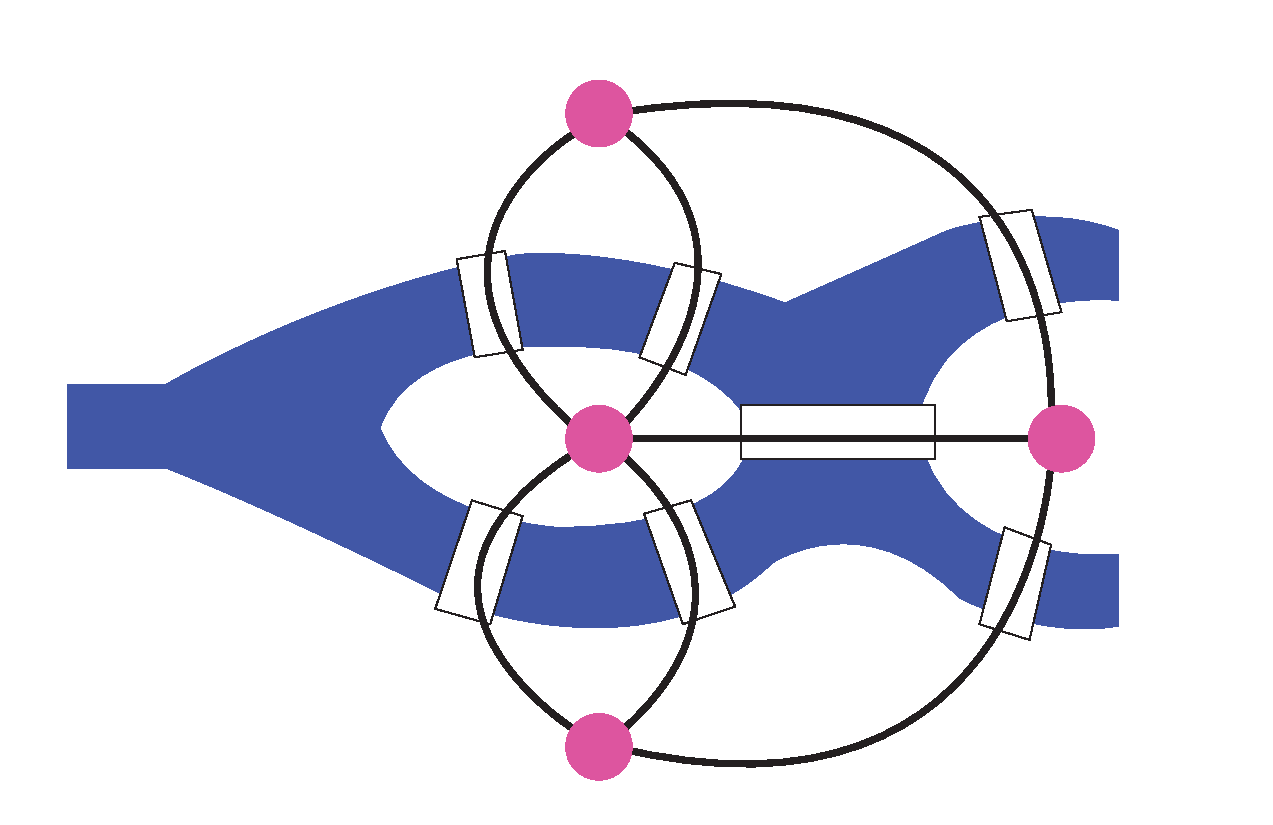
\includegraphics[width=4in]{assets/7bridges.pdf}
%  \caption{Illustration of the Seven Bridges of Köningsberg as a graph}
%  \label{fig:7bridgesIllustration}
%\end{figure}

%\begin{figure}[H]
%  \centering
%  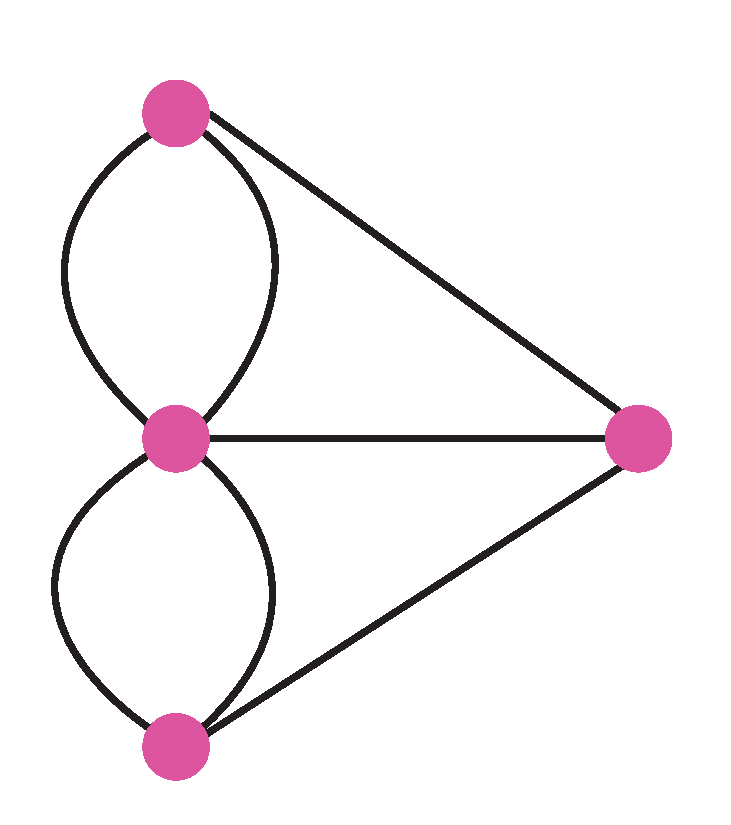
\includegraphics[width=2in]{assets/7bridges2.pdf}
%  \caption{Illustration of the Seven Bridges of Köningsberg as a simplified graph} 
%  \label{fig:7bridgesSimplification}
%\end{figure}

Graph databases use graph structures for semantic queries with nodes, edges, and properties to represent and store data.
The nodes represent entities, such as people, accounts, or bus stops, while the edges represent the relationships, such as ``Friend of'' or ``Belongs to'', between the nodes. A property is relevant information that can relate to either a node or an edge, such as ``Name'' or ``Travel Time''.
%Må omformuleres
Applications of graph databases can include calculating routes and finding the shortest path between locations in a network, such as a road or rail network, airspace network, or logistical network \citep[p.102]{robinson13}. 
%Må omformuleres Compared to relational databases, are graph databases often faster for associative data sets, and map more directly to the structure of object-oriented applications. They can scale more naturally to large data sets as they do not typically require extensive join operations. A drawback to graph databases is the inertia of finding all objects of a specific type.  The following operations are not recommended using graph databases: large, set-oriented wueries, graph global operations and simple, aggregate-oriented queries\citep[p. 40-41]{bruggen14}

\subsection{Neo4j}
\label{subsubsec:neo4j}
Neo4j \citep{website:neo4j} is an open-source graph database, implemented in Java. It is ranked the most popular graph database worldwide \citep{website:graphdbranking} and is used by several large companies such as Telenor \citep{website:telenor}, Walmart \citep{website:walmart} and Cisco \citep{website:cisco}. It is a native graph database optimized and designed for storing and managing graphs and is known for extremely fast traversals of relationship. The underlying data model of Neo4j is the labeled property graph and is one of the most generic and versatile of all graph models \citep[p.73]{robinson13}. This graph data model gives four different fundamental building blocks to structure and store data. These building blocks includes Nodes to store entity information, Relationships to connect nodes to another, Properties for relevant information, and Labels for creating subgraphs.

A query that is extremely well suited for graph databases are queries for finding the paths between different nodes in a graph. Neo4j can be used to see whether a path exists, finding the optimal path, and looking for variability in the path \citep[p. 51]{bruggen14}. Neo4j includes built-in methods for finding the shortest path, including Dijkstra's algorithm. Dijkstra's algorithm \citep[p.658-662]{cormen09} maintains a set $S$ of vertices' whose final shortest-path weights from the source $s$ have already been determined. The algorithm repeatedly selects the vertex $u = V - S$ with the minimum shortest path estimate, adds $u$ to $S$, and relaxes\footnote{Making a change that reduces constraints.} all edges leaving $u$. The running time of Dijkstra's algorithm is $O((V + E)log V)$ and it is guaranteed to find the shortest path \citep[p.~661]{cormen09}. %Dijkstra is one of the best-known algorithms to calculate the shortest weighted path between two points on a graph, using the properties of the edges as a weight or costs. 
The Relationships in a Neo4j database are capable of being of different RelationshipTypes that, among others, enables the built-in Dijkstra to find the shortest path using only specific RelationshipTypes.

%Sweet spot use cases of neo4j: complex, join-intensive queries, path finding queries\citep[p. 51]{bruggen14}. 

%TODO skrive mer her

%Advantages:
%\begin{itemize} 
%\item Flexibility: model, develop and visualize the world as you experience it. Its simply nodes and relationships. 
%\item Performance: Hyper-connectivity at speed. 
%\item Scalability: Scales up and out, supporting tens of billions of nodes and relationships, and hundred of thousands of ACID transactions per seconds. 
%\item Speed: Able to search trough millions of connections per second, with real time queries that stay fast even as your database grows. 
%\end{itemize}

%\begin{itemize}
%\item Native graph database. 
%\item Property graph. 
%\item Made for real time queries. 
%\item Really fast traversals of relations.
%\item Neo4J has an API that supports traversing - finding shortest path - can weight edges, nodes -
%\end{itemize}
%//en korteste vei mellom n og m men max lengde 3
%match p = shortestPath ( (n) - [*...3]--(m)) return p
%(Vekte kanter: Neo44J har et API som støtter traversering, Dijkstras er innebyd ++ som lar deg vekte kanter - hva er raskeste vei ++)

%Neo4J can be used to evaluate routes after the ants have created route sets.
%\section{Motivation}

Trondheim and neighboring municipalities are among the areas with the greatest population growth in Norway \citep{website:miljopakken}. More people means more traffic, and without action will congestion and environmental problems increase every year. 

Private transportation have many advantages for the citizens compared to the public ones. They do not have to wait for a vehicle at the beginning of a trip, change vehicles during the trip, and it is often more convenient. The negative issues of private transportation, such as traffic jams and increased travel times, means increased air pollution, noise and accidents. 

Having efficient public transportation systems can substantially reduce negative effects of private transportation networks 
\citep{kechagiopoulos13} . The environment package \citep{website:miljopakken} for transport in Trondheim involves providing better road networks and public transport. With this they hope to achieve lower emissions, shorter traffic jams and less traffic noise. Inadequately designed transit network can cause very long waiting times and increase uncertainty in bus arriving time \citep{nikolic14}. Therefore, public transportation systems should be improved by providing better travel services, and inform the public about them, in order to convince more people to travel with it instead of using their own car. 

 \citet{website:atb} is responsible for planning the public transport throughout Sør-Trøndelag County. \textit{Among public transportation alternatives, “bus” has specific attractive features. These are flexible routes, medium capacity, low cost (of capital and running), easy implementation, flexible fleet size (easy to expand or contract this size), and use of existing facilities (roads and streets).} In Trondheim, bus services comprise the major component of public transportation system. From a meeting with AtB we learned that the current solution of AtB consists of an experience based route network, where no common methodology is used, and where all bus route networks and schedules are designed manually. As a result, the efficiency of the resulting networks is highly dependent of the designers expedience and his / hers knowledge of existing resource constraints and transportation demands. Satisfying all customer needs, and keeping all operator costs in check, is really difficult to achieve \citep{kechagiopoulos13}. Operator costs mainly refer to the total number of buses, total bus running distance and the total operation hours. A minimum trip time, amount of transitions, and a not too crowded bus (customers can tolerate standing in 15 minutes ) are among the most important factors that determine the passengers choice of public transit, AtB experiences.  \textit{The main concern of bus companies is maximizing its profits, while the main concern of the government is to fulfill all needs of traveling in public} \citep{kechagiopoulos13}. The manual attempts to provide an acceptable solution the Vehicle Routing Problem are not able to solve these large network problems efficiently \citep{kechagiopoulos13}. 

 \textit{The number of journal publications on Vehicle Routing Problems has steadily increased over the years. This is because of the progress in computational resources has opened new possibilities for modeling more complex routing problems. New arising real-world applications provide inspiration for developing new approaches for coordinating complex transportation processes.}  \citep{vehiclerouting}




















\chapter{Preparatory Research}
\label{relatedWork}
%%Må skrives om
This chapter describes the preparatory research done in order to develop the proposed method. Section \vref{sec:definingResearchTopic} defines the research topic used in order to guide the Structured Literature Review\citep{kofod2014}, which further is described in Section \vref{sec:structuredLiteratureReview}. Section \vref{sec:relatedWork} reviews the relevant studied and will answer Research Question \vref{itm:1} as a whole. Finally, in Section \vref{subsec:problemStatement}, Research Question \vref{itm:2} and \vref{itm:3} are defined based on the answers of Research Question \vref{itm:1}.  

\section{Refining the Research Topic}
\label{sec:refiningResearchTopic}
\citet{cohen88} introduced a five-stage model for evaluating research in terms of a five-stage cycle. The development process should be run in iterative cycles, and the suggested model is used for evaluation throughout the project. The first stage in the model involves refining the research topic to a task, and identifying a view of how to accomplish the task. %The rest of the stages will be evaluated in Section \vref{subsec:evaluationCriteraCohen}. 
As stated in the motivation, Section \vref{sec:motivation}, congestion and environmental problems in Trondheim is increasing every year due to the population growth\citep{website:miljopakken}, and efficient public transportation systems can reduce the negative effects of these issues. Since AtB's\citep{website:atb} current solution consist of an experience based route network, may it not be the optimal solution. The task in this research is to optimize urban transit networks using swarm intelligence methods. Further, is the goal to make urban transit networks more convenient for passengers, and thus increase the number of public transportation passengers in Trondheim. 

A Structured Literature Review, based on the model suggested by \citet{kofod2014} is conducted to gather available information from primary relevant studies.

\section{Structured Literature Review}
\label{sec:structuredLiteratureReview}

The urban transit network design problem (UTNDP), is suggested to be solved using swarm intelligence (SI) to develop an algorithm. As described in Section \vref{sec:VRP}, is UTNDP a sub-problem of the vehicle routing problem (VRP), which is a generic name given to a broad class of optimization problems. VRPs are represented as a road network by relevant locations in a graph, and graph databases uses graph structures to represent and store data. For these reasons, %will we  determine previous research in solving VRPs using SI methods and whether graph databases are employed in combination with the VRP and SI. 
were the following research questions formed in order to guide the review:

\begin{enumerate}[label=\textbf{\arabic*})]
\item 
    \begin{enumerate}
    \item Is SI methods suitable for the VRP?
    \item What is the state-of-the-art in solving VRPs using SI methods?
    \item What changes have been done to the classical SI methods to improve them?
    \item Have there been any attempts to combine different SI methods?
    \item Have graph databases been employed in combination with the VRP and SI?
    \end{enumerate}
\end{enumerate}

Key search terms were decided based on the defined research questions, formed into groups of synonyms, and assembled into a complete search term. The key search terms and the complete search term can be found in appendix \ref{appendixA}, section \vref{searchterm} and section \vref{sec:searchTerms}, respectively. The list of sources for retrieving the  relevant literature, were selected based on \citep[p.3]{kofod2014}, and can be found in Appendix \vref{appendixB}. 

To exclude irrelevant literature, some Inclusion Criteria was decided to ensure a level of relevance. The Inclusion Criteria can be found in Appendix \ref{appendixA}, Section \ref{sec:inclusionCriteria}. After the Inclusion Criteria filtering, we had 42 sources for the related literature, including scientific papers and master theses. Quality Criteria was determined to ensure quality in the final papers and to filter away studies not theoretically relevant for our thesis. Each of the studies under consideration was classified according to the Quality Criteria, by scoring the papers on each Quality Criteria. Each point was given a score, where 1 point denote relevant, $\frac{1}{2}$ point denote partly relevant and 0 points denote not relevant. For retrieving the most relevant papers based on the content and not just the quality of the paper, Quality Criteria \ref{itm:qa1a} and \vref{itm:qa1b} was multiplied by 3. Quality Criteria \ref{itm:qa1a} is concerned about whether or not the research in fact is a Vehicle Routing Problem and Quality Criteria \ref{itm:qa1b} addresses whether or not swarm intelligence is the main optimization method. 

Table \vref{table:literature} shows the papers that were selected based on the Inclusion Criteria and the scores given based on Quality Criteria. The average score of the read literature was 13.01 $\approx$ 13, and literature given a score $\geq{1.5}$ above average were selected. This resulted in 12 final researches, which can be seen in Table \vref{table:finalliterature}. This research will form the foundation of the thesis. Section \vref{sec:relatedWork} are the results of the final data synthesis, and they all describe a vehicle routing problem attempted solved by a swarm inspired method.

\section{Related work}
\label{sec:relatedWork}

%The research gathered from the SLR will form the foundation of the thesis, and this Section is the results of the final data synthesis, 

%\newline
%----------------------------- solving VRPs using swarm intelligence using car transirtation

\subsection{Vehicle Routing Problems}
\label{subsec:relatedWorkVRP}

As stated, all the retrieved literature from the structured literature review has studied the possibility of solving VRPs using swarm intelligence. \citet{hsiao04}, \citet{salehi-nezhad07}, \citet{tripathi09}, \citet{dias14}, \citet{salehinejad10}, and \citet{sedighpour14} all use swarm intelligence to solve vehicle routing problems involving cars transporting either persons or goods.

%Mangler informasjon om algoritmene som sammenlignes med. Parametersettingen er beskrevet, men ikke forklart. 
\citet{hsiao04} presented an approach to search for the best path of a map considering the traffic loading conditions. To do this, they proposed an ACO algorithm to search for the shortest path from a desired origin to a desired destination. The presented algorithm is a classic ACO algorithm without changes and compared their algorithm to a brute method emphasizing on the time used to generate the route. Their results state that if the map consists of more than 200 nodes, the ACO performs better than a brute method. In fact, they found that the more nodes the map contains, the higher the benefit of using the ACO algorithm. 

\citet{salehi-nezhad07} presented an ACO algorithm to search for the best path between two desired intersections in cities, called Ant-based Vehicle Navigation algorithm. To get more accurate results than a standard ACO algorithm they employed a \textit{awarding/punishment}-method. The path found by the ``best ants'' are given more pheromone than the path of the ``bad ants''. In order to find the best path, the presented algorithm is concerned about the parameters \textit{distance}, \textit{width}, \textit{traffic load}, \textit{road risk}, \textit{road quality}, and \textit{number of intersections}. The algorithm was applied on a part of the city of Kerman, and the results are encouraging and well described. The algorithm provides a fast access, low cost and easy method for vehicle navigation in cities without assisting GPS.

%Mangler informasjon om algoritmene som sammenlignes med
\citet{tripathi09} solved the vehicle routing problem with stochastic demand, in which the customer demand is modeled as a stochastic variable. They performed this using an improved version of ACO, called ns-AAA SO. The proposed algorithm orients the search progressively towards favoring the global optimal solution. To do this they define that a complete iteration consists of two tours: The first tour is a social tour that corresponds to a standard ACO iteration. The second tour is a neighborhood tour where the ants are allowed to communicate important information found in the social tour and change their solutions. If the fitness value of the new solution is better, the old solution found in the social tour is replaced. To favor the optimal solution, the path of the global best path is given more pheromones. Further, to prevent the search from entrapment into a local optima, a minimum quantity of pheromone on any edge, $t_{min}$, is always maintained. The performance of ns-AAA SO was compared with both a standard ACO algorithm and a genetic algorithm. They found that ns-AAA SO outperforms the other two algorithms in every problem instance described by the authors.

%Mandler informasjon om parametersetting
\citet{dias14} introduced an inverted ACO (IACO) algorithm. The idea is that the IACO algorithm inverts the logic of the classical ACO algorithm by converting the attraction of ants towards pheromones into a repulsion effect. The proposed approach was used in a decentralized traffic management system, where the drivers acted as the inverted ants. The drivers were repelled by the scent of pheromones (other drivers), and the system thus avoids congested roads. The described approach was compared to a shortest-time algorithm (ST), and the IACO algorithm performs better than the ST algorithm with the respect to trip time, travel length, fuel consumption and $CO_2$ emissions. This is as long as a considerable amount (25-50\%) of the vehicles uses the inverted ant algorithm to decide which road to choose. 


%Parameterne er nevnt og den sammenligner med relevante algoritmer.
\citet{salehinejad10} introduced a route selection system that uses an Ant Colony System (AS), as described in Section \vref{subsec:aco}, to detect an optimum multiparameter direction between two desired points in urban areas. Their algorithm is called Fuzzy Logic-Ant Colony System (FLACS). FLACS differs from other ACSs by the employment of fuzzy logic for the local pheromone updating. The proposed system is concerned about the parameters \textit{Distance}, \textit{Traffic Flow}, and \textit{Incident Risk} on each edge. FLACS also implements a tabu list, where visited nodes are added to avoid cycles. The system is applied to a part of London, United Kingdom, consisting of 42 junctions. Their proposed system is compared to a standard ACS and a $A^*$-ACS emphasizing on the parameters mentioned above. They found that FLACS performed better at average than both systems regarding operational cost, regardless of the importance in the parameters. It is worth mentioning, the estimation of further traffic data is done by artificial neural networks, and the traffic data for each system is not exactly the same.
%They found that FLACS has less running time than $A^*$-ACS, but more than the standard ACS due to its Fuzzy Logic system component. 

%Sammenligner ikke algoritmen mot original ACO, selvom de sier at de ønsker å forbedre ACO i introduksjonen
\citet{sedighpour14} introduced a hybrid ACO (HACO) algorithm to solve the open vehicle routing problem (OVRP). This is a subproblem of the classical VRP where the vehicles are not required to return to the depot. To overcome some of the shortcomings of the original ACO, such as slow computing speed and local convergence, they made three improvements. First they equipped each node with a candidate list containing nodes nearby that had not yet been visited. Second,  they applied several local search techniques to the \textit{n} best solutions found each iteration to improve them further. Third, they decided the amount of released pheromone based on the rank of the best-known solution found so far. The HACO algorithm was compared with three versions of PSO (standard PSO, PSO without one-point move (PSOWO) and PSO without neighbors (PSOWN) regarding performance. The algorithms were tested on fifteen different sets, consisting of 19 to 72 nodes with 2 to 7 vehicles fixed at the minimum possible. Their result table shows that HACO performs better than the others regardless of the test case used.

\subsection{Urban Transit Network Design Problems}
\label{subsec:relatedWorkUTNDP}

Urban Transit Network Design Problem (UTNDP), a subproblem of VRP, considers other objectives and requires other methods for generating solutions than classical VRP problems. As mentioned in Section \vref{sec: VRP}, UTNDP is divided into two parts. The first part includes creating urban transit routes on existing networks (UTRP) and the second part involves the development of schedules (UTSP). \citet{yang07}, \citet{jiang10}, \citet{poorzahedy11}, \citet{nikolic14}, and \citet{kechagiopoulos14} all describes solutions related UTNDP. %The aim of UTRP is generally to minimize the average trip time by maximizing the number of direct travelers per unit lengths.

%Parameterne er nevnt og den sammenligner med relevante algoritmer
\citet{yang07} presented an optimization algorithm for an urban bus network design (UBND), a problem closely related to the UTNDP. This algorithm is based on \citet{dorigo96}s Ant Colony Algorithm (ACA), called coarse-grain parallel ant colony algorithm (CPACA). CPACA is very similar to the original ACA, but it applies less communication between the ants by dividing the colony of ants into sub-colonies that runs in parallel and only communicate with each other. Their results are compared with the classical MAX-MIN ant system (MMAS)\citep{stutzle99} and with ACA with Ant-weight strategy (ACA+). They found that CPACA performed best regarding both average direct traveler density and run time. 

%Parameterne er nevnt, men ikke begrunnet. Sammenligner med relevante algoritmer. 
\citet{jiang10} describes an improved ACO (IACO) algorithm to solve the UTRP. The specific improvement made to the algorithm is the implementation of a stagnation counter to determine whether the algorithm has fallen into stagnation. When there is no better solution found after an iteration, the stagnation will increase by 1. When the stagnation counter reaches a certain threshold, the pheromone levels associated with each edge is reinitialized. This improvement is done to compensate for the classical ACOs shortcomings of easily falling into stagnation and, therefore, obtain a local optimal solution. The IACO algorithm is, as the algorithm described by \citet{yang07}, compared to the classical MMAS. The results show significant improvement to the convergence speed compared to MMAS. The also found that IACO performed better both regarding average number of iterations and average path distance. 

%Parameterne er nevnt, diskutert og begrunnet. Sammenligner for så vidt med relevante algoritme (GA).
\citet{poorzahedy11} proposed an Ant System for solving the bus network design problem (BNDP). BNDP is defined as the study of choosing a subset of interconnected bus routes among a given set of such routes. A successful solving of the BNDP, similar to UTNDP, minimizes the total travel time of the users of the network and the operational cost. Like the FLACS algorithm proposed by \citet{salehinejad10} and described in Section \vref{subsec:relatedWorkVRP}, the proposed AS algorithm also employs a tabu list for each ant where visited nodes are added. Their solution generates multiple nests across the transit network and each nest is responsible for creating a subnetwork, which is combined to a complete bus network at the end. The system is only concerned about one objective; a combination of travel time for the users and the bus fleet size for the operator. The application was used to design the bus network of Mashhad and was further be compared with a genetic algorithm (GA). Their results show that their system performs better than the GA in both the number of routes, fleet size, in-vehicle travel time and waiting time. Both the GA and the AS performs significantly better than the existing solution on all measures.  

%Parameterne er nevnt, men ikke begrunnet. Sammenligner med relevante algoritmer. 
\citet{nikolic14} proposed a method for solving the UTNDP. To do this, they used an improved version of the original BCO \citep{lucic03}. The bees start with an initial solution at each iteration, where the initial solution is the best-known solution so far. The initial solution is only updated if a better solution is found. The method was tested on Mandl's benchmark problem of a Swiss bus network\citep{mandl80} and compared to competitive approaches (\citet{mandl80}; \citet{shih94}; \citet{baaj95}; \citet{bagloee11}). The performance criteria used to measure the performance was regard to the percentage of total transfer demands satisfied directly ($d_0$), with one transfer ($d_1$), two transfers ($d_2$), or with more than two transfers or not satisfied at all ($d_{unsat}$). The methods are also compared regarding total in-vehicle travel time. The experiments are conducted on route set designs with four, six, seven and eight routes. They found that the proposed method performed best regarding total travel time and number of transfers if the order of importance was set to favor the passengers and the number of lines were greater than 4. If the order of importance was set to favor what was best for the operator, the method created the solution with the smallest fleet size independent of number of lines, otherwise the method performed mediocre regarding all the other measures. 

%Parameterne er nevnt, diskutert og begrunnet. Sammenligner med relevante algoritmer.
\citet{kechagiopoulos14} designed and presented an original PSO algorithm without any changes or improvements. Their goal was to find an efficient solution to the UTRP. The target problem was, like \citet{nikolic14}, Mandl's benchmark problem, and their algorithm was compared with competitive approaches, including genetic algorithms and other metaheuristic approaches mentioned in literature (\citet{baaj91}; \citet{chakroborty02}; \citet{kidwai98}; \citet{fan10}; \citet{fan09-2}; \citet{zhang10}; \citet{chew12}). The algorithms were compared to the same performance criteria and the same amount of route set sizes as \citet{nikolic14}, but instead of comparing total in-vehicle time, they used the average in-vehicle time experienced by each passenger ($ATT$). They found that the proposed algorithm performs better than the competitors regarding $ATT$ independent the route size and achieves a better percentage of direct travelers ($d_0$) except when the route set size was four. 

\subsection{Discussion}

Based on the proposed literature review we see that swarm intelligence inspired system has proven to be useful solving multiple vehicle routing problems. During the past decade, there has been published several research on the subject and many of these reports promising results. 

We see that a lot of the newest published research addresses the weaknesses of classical SI-methods and makes changes to the original algorithms to overcome some of these weaknesses. In these cases we believe the conducted experiments should include comparison with the respective swarm method to indicate whether or not their solution improved the addressed shortcomings. \citet{tripathi09}, \citet{yang07}, \citet{salehinejad10}, and \citet{jiang10} all presented research where their swarm intelligence inspired algorithms were designed to overcome some of the known weaknesses. They compared their solutions with other corresponding swarm methods, achieving promising results. Because of this comparison, they can conclude whether or not the addressed weaknesses are improved. \citet{sedighpour14} improved the classic ACO to overcome slow computational speed and local convergence. However, they did not compare the proposed algorithm to other implementations of ACO, and the research will not be valid to conclude whether or not it actually overcomes some of ACO's weaknesses. 
Neither \citet{dias14} nor \citet{poorzahedy11} tests their solution against other swarm intelligence methods, but against other reasonable algorithms, respectively a Shortest Time-algorithm and a GA. The comparison against GA in \citet{poorzahedy11} is descriptive because they did not add additional features, other than a tabu list of all visited nodes, to the AS algorithm. In \citet{dias14}'s research, it makes sense to only test against an ST-algorithm, because they inverted the core factor of ACO. A comparison against a standard ACO would, therefore, be non-descriptive. \citet{salehi-nezhad07} did not compare their algorithm against any other algorithm at all, which makes their results hard to verify. 

The performance of metaheuristic methods, including swarm inspired methods, are highly dependent on their parameter settings. The process of parameter tuning is an important contribution to the field of swarm intelligence in general. Several researches, including \citet{salehi-nezhad07} and \citet{yang07}, describes their parameter setting as a product of ``trial and error''. We consider this to be a weakness of their research because it is not possible to validate their results. \citet{sedighpour14}, \citet{poorzahedy11}, and \citet{kechagiopoulos14} discussed and justified their parameter settings by conducting their experiments in two parts; one for parameter setting and one for performance. We consider this is a strength of their research. 

The size of the test cases used is an important factor in determining both scalability and robustness of the proposed algorithm. \citet{nikolic14} and \citet{kechagiopoulos14} both uses Mandl's benchmark problem as input. This benchmark problem, presented in Fig. \vref{fig:MandlNetwork_problemstatement},  is a small network containing 15 nodes and 21 edges.  Mandl's network is widely used and acknowledged by multiple researchers, including \citet{baaj91}, \citet{chakroborty02}, and \citet{fan09}. This is a strength of their research because it enables comparison of their results to a numerous of other solutions using the same benchmark problem. However, as mentioned, the Mandl network is quite small. The robustness of their algorithms regarding both time and space complexity could have been verified by also applying their algorithm to a larger test case. \citet{salehi-nezhad07} also applied their solution to a small test set, containing only 27 intersections and requiring only 5 ants and, like the authors that used the Mandl Network, the robustness could have been verified by also applying the algorithm to a larger test set.  

\subsection{Conclusion}
\label{subsec:relatedWorkConclusion}

Based on a review of the related work the first research question can be answered:

\subsubsection*{RQ 1: What is the state-of-the-art in solving vehicle routing problems using swarm intelligence methods and graph databases?}

%Swarm intelligence methods are suitable for solving vehicle routing problems. \citet{tripathi09}, \citet{dias14}, \citet{poorzahedy11}, \citet{nikolic14}, and \citet{kechagiopoulos14} all compared their algorithm against other approaches than SI and found that the proposed SI-algorithms generally performed better.
The structured literature review did not retrieve any previous research that used graph databases in combination with the vehicle routing problem and swarm intelligence. The state-of-the-art of solving vehicle routing problems using swarm intelligence methods can be summed up to  being inspired by original SI-methods, but to add and remove features to make the methods more suited for the tasks. Ten out of the eleven reviewed papers made changes to the original method. We notice a trend of implementing a notion of the best known solution so far, and using this to either directly or indirectly improve the solutions created by the individuals of the swarm \citep{tripathi09,sedighpour14,nikolic14}. 



%\citet{tripathi09}, \citet{yang07}, \citet{salehinejad10}, and \citet{jiang10} compared to ACO
% citet{nikolic14} and \citet{kechagiopoulos14} mandl



\section{Problem Statement}
\label{sec:problemStatement}

\emph{\color{blue} TODO: referansene må oppdateres.}

%\begin{itemize}
%\item \citet{cohen88} \textbf{asks, how is your reformulation / method an improvement? And underlying assumptions.}

ACO has several advantages for the VRP, such as natural parallelism and continuous positive feedback, which allows good solutions to be identified fast. However, ACO also has a few drawbacks including the weakness of getting stuck at a local optima. We will investigate the possibility of overcoming this drawback by improving ACO, and including features from other swarm inspired methods. As stated in Section \vref{sec:relatedWork}, we only found one attempt to combine different methods from swarm intelligence.% is to add a notion of the global best solution found to ACO and BCO. 

We did not manage to find any previous research that used graph databases in combination with the vehicle routing problem and swarm intelligence. As mentioned in \vref{subsubsec:neo4j}, does the graph database Neo4j \citep{website:neo4j} have several advantageous features for managing graphs, and we will therefore determine potential advantages and disadvantages of using Neo4j in our implementation and in the optimization process, giving us research question \vref{itm:3a}.

%\item \citet{cohen88} \textbf{asks if any aspects have been abstracted away?}

%As mentioned, does the UTRP comprise the design of physical transportation routes needed to solve the UTNDP. UTSP involves the development of schedules. We will in this thesis focus on UTRP. Geographical issues.
%and the objective in this thesis will therefore be to minimize the total travel time in the public transportation system, by optimizing the routes concerning the travel time and minimizing number of transfers.
The current solution of AtB consist of an experience based route network, and therefore not properly, computationally optimized concerning the travel demand and travel time. When a route network is not properly optimized, it can lead to a large number of transfers for passengers when they are traveling from their origin to their destination, resulting in a long total travel time. A good route network will ensure that routes having the most traveling demands are satisfied with short paths and few vehicle transfers, making travel demand a key variable for the algorithm. AtB\citep{website:atb} does not possess accurate data about the travel demand, and detailed investigations into measuring and predicting travel demand is a complex research problem, and beyond the scope of (and abstracted away\citep{cohen88} from) this thesis. 
%\item \citet{cohen88} \textbf{Does it rely on other methods?}

Demand values are all provided for Mandl's benchmark problem\citep{mandl79}. This benchmark problem seems to be the only one widely used for the UTRP and is acknowledged by researchers\citep{fan09},\citep{kechagiopoulos14},\citep{nikolic14}. Christoph Mandl\citep{mandl79} developed a heuristic algorithm for the UTRP, and the method was applied and based on a real network in Switzerland, the Swiss transit network\citep{mandl80}. The data includes a small and dense network with 15 nodes and 21 edges, in addition to the travel times and travel demand for each edge, and will in this thesis be used as the input data. %The total demand is 15570 trips per day, which is a relatively high demand for a small network. The travel time between the to farthest nodes in the network is 22 minutes along the shortest path. 

%Mandl developed a solution in two phases, where a feasible set of routes were created in the first phase and in the second phase he tried to minimize the the total travel time, including in-vehicle time and waiting time, by reducing the number of transfers. Some important measures of Mandl's solution network includes, for example, 100\% service coverage, 69.4\% of the trips involving no transfers, 29.93\% of the trips involving one transfer, and only 0.13\% of the trips needing more than one transfer. 

%\item \citet{cohen88} \textbf{asks when have you successfully demonstrated a solution? Is there a recognized metric for evaluating the performance?}

In order to demonstrate a solution we will evaluate the performance of our algorithm against the performance criteria used in similar research for comparison[\citep{kechagiopoulos14},\citep{mandl80},\citep{nikolic14},\citep{fan09}], and are the following:
\begin{itemize}
\item The percentage of demand satisfied without any transfers, which should be as high as possible.
\item The percentage of total transfer demands where the number of transfers are 1, which should be as low as possible.
\item The percentage of total transfer demands where the number of transfers are 2, which should be as low as possible.
\item The percentage of unsatisfied travelers, which should be equal to zero. An unsatisfied traveler is described as a traveler with 3 or more transfers.
\item The average travel time in minutes per transit user, which should be as low as possible. %The travel times incorporates a transfer penalty, which is sat to be 5 minutes per transfer for comparison reasons. 
\end{itemize}

%\item \citet{cohen88} \textbf{asks is the research is representative for a class of tasks? What is the scope of the method?}
%Does it transfer to more complicated problems?
For the reasons stated above, (the scope of the research) we will in this thesis focus on the UTRP, creating effective urban transit routes, with an ACO algorithm inspired by both BCO and PSO. (Comparing our results with Mandl etc.) This will help us establish Research Question \vref{itm:2a}, which is concerned about whether or not it is efficient to combine attributes from different swarm intelligence methods in order to improve the computational results.

Our goal with our implementation is that it further can be used to optimize AtBs transit network in order to increase the number of public transportation passengers. Research Question \vref{itm:2c} is concerned about whether or not it is possible to apply our algorithm to optimize bus routes in urban cities. This question cannot be fully answered until it is applied to an urban city, but we will strive to create a method that is easily adaptable with the concerns of public transportation in cities in mind. The implementation will be easily changed with new demand values, and tested on other larger networks.
%\end{itemize}



\chapter{The Proposed System}
\label{theModel}
Here you will present the architecture or model that you have chosen and that is (or will be) implemented in your work. Note that putting algorithms in your report is not desirable but in certain cases these might be placed in the appendix. Code further be avoided in the report itself but may be delivered in the fashion requested by the supervisor or, in the case of masters delivery, submitted as additional documents. 

\textit{This is the main structure of what you built.
- Not at code level, but you can include pseudocode.
Explain the system in a way the reader understands it.
Include diagrams and the algorithms used.}

TODO: Skrive om hvorfor vi har valgt å kode i java. speed, vi kan det best, (ne04j) ++

\section{Input Data}

%TODO: Referanser til hvor vi lastet ned dataen

We have designed and implemented a method to produce a realistic transit network based on the data from Mandl \citep{mandl79}. The transportation time on each edge is given, and the transportation demand is assumed to be known and constant. 

To do this we have constructed a transit network, including edges and nodes, based on the data set we have downloaded from \
citet{fan09}, which consist of text files:




\begin{table}[h!]

    \begin{tabular}{|l|lr|}

 	\hline
 	~ & x & y \\
 	\hline
    1 & 1 & 9 \\
    2 & 3 & 8 \\
    3 & 4.5 & 7.75 \\
    4 & 2.75 & 6.2 \\
    5 & 0.8 & 6.6 \\
    6 & 4.6 & 6 \\
    7 & 7 & 4.5 \\
    8 & 5.5 & 5 \\
    9 & 8.5 & 6.8 \\
    10 & 5.8 & 2.25 \\
    11 & 3.8 & 2.25 \\
    12 & 1.3 & 3.5 \\
	13 & 5.25 & 1 \\
	14 & 6.7 & 1.75 \\
	15 & 6.75 & 5.8 \\
	\hline
    \end{tabular}
    \caption {Mandl Coordinates}
\textit{The MandlCoord.txt file includes 15 lines, with the (x,y) coordinates of the 15 nodes. These coordinates was not supplied in Mandl's literature, so these are copied from \citet{fan09} and are approximate for the picture to be drawn.}
\end{table}


\begin{table}[h!]
    \begin{tabular}{|l|lllllllllllllll|}
    \hline
    ~ & 1       & 2        &  3    &   4     &  5     &  6      & 7      &  8     & 9      & 10      & 11     & 12         &  13     & 14       &  15  \\
    \hline
    1 & 0       & 8        &  Inf    &   Inf     &  Inf     &  Inf      & Inf      &  Inf     & Inf      & Inf      & Inf     & Inf         &  Inf     & Inf       &  Inf  \\
    2 &8       & 0        & 2       &  3        &  6       &  Inf      & Inf      & Inf      & Inf      & Inf      & Inf     & Inf         &  Inf     &  Inf      &  Inf  \\
    3 & Inf     &  2       &  0      &  Inf      & Inf      &  3        &  Inf     &  Inf     & Inf      &  Inf     & Inf     &  Inf        &  Inf     &   Inf     & Inf   \\
    4 & Inf     &  3       &  Inf    &  0        & 4        & 4         & Inf      &  Inf     &  Inf     & Inf      & Inf     & 10          &  Inf     &  Inf      &  Inf  \\
    5 & Inf     &   6      &   Inf   &    4      &   0      & Inf       &  Inf     &  Inf     &   Inf    &   Inf    &    Inf  &     Inf     & Inf      & Inf       & Inf   \\
    6 & Inf     & Inf      &   3     & 4         &  Inf     &  0        &   Inf    &    2     & Inf      & Inf      & Inf     & Inf         & Inf      & Inf       & 3     \\
    7 & Inf     & Inf      &  Inf    &   Inf     &   Inf    &   Inf     & 0        & Inf      &  Inf     &  7       & Inf     & Inf         & Inf      & Inf       &  2    \\
    8 & Inf     & Inf      & Inf     & Inf       & Inf      & 2         & Inf      &  0       &  Inf     &  8       & Inf     &  Inf        &  Inf     & Inf       & 2     \\
    9 & Inf     &  Inf     & Inf     &   Inf     & Inf      & Inf       &  Inf     &  Inf     & 0        &  Inf     & Inf     & Inf         & Inf      & Inf       & 8     \\
    10 & Inf     &  Inf     & Inf     &  Inf      & Inf      &  Inf      & 7        &  8       &  Inf     &  0       & 5       & Inf         & 10       & 8         & Inf   \\
    11 & Inf     &  Inf     & Inf     & Inf       &  Inf     &  Inf      & Inf      & Inf      &  Inf     &   5      & 0       & 10          &  5       & Inf       & Inf   \\
    12 & Inf     & Inf      & Inf     & 10        & Inf      & Inf       & Inf      &  Inf     &  Inf     &  Inf     &  10     & 0           & Inf      & Inf       & Inf   \\
    13 & Inf     & Inf      & Inf     &  Inf      &  Inf     & Inf       &  Inf     &  Inf     &  Inf     & 10       &  5      & Inf         &  0       & 2         &  Inf  \\
    14 & Inf     & Inf      &  Inf    &  Inf      &  Inf     & Inf       &  Inf     & Inf      & Inf      & 8        &  Inf    &  Inf        & 2        & 0         &   Inf \\
    15 & Inf     & Inf      & Inf     & Inf       & Inf      & 3         &  2       &  2       & 8        & Inf      & Inf     &
     Inf         &  Inf     & Inf       &  0    \\
     \hline
    \end{tabular}
    \caption {Mandl Travel Times}
    \textit{MandlTravelTimes.txt The travel times matrix gives the travel times it takes in minutes between the nodes. This matrix is symmetrical, travel times between each node and itself are zero, and ``Inf'' indicates that there is no direct link between the nodes.}
\end{table}



\textbf{MandlDemand.txt} - The demand matrix shows the travel demand between each node pair, which is the average number of passenger trips per day. This matrix is also symmetrical. (These is no demand either to or from node 15, but it is always included in the route sets because the rules that are used insist on every node being included \citep{fan09}. For coding reasons, we changed the numbers in the main diagonal (from to left corner to bottom right corner) from all zero to all ’a’s. 






\subsection{Route set representation}

The nodes we create includes their coordinates, and a ant number to distinguish the ants from each other. 
The edges we create includes the travel time between and the demand between two nodes. 
%We have made edges based on the demand for each node, even though there is no direct link (travel time) between these two nodes. %TODO: skrive om hvordan vi gjør det når maurene skal velge kanter basert på travel time. But these edges has the value -1, meaning there is no direct link between the nodes. 
The travel time indicates whether there is a direct link. %TODO: skrive mer her.  
In addition to travel time and demand, each edge includes a pheromone value to be updated after the algorithm is executed.

\begin{figure}[hb]
  \centering
  \includegraphics[width=4in]{assets/mandlnetwork.png}
  \caption[Transit Network]
   {The Transit Network, including 15 nodes and 21 edges. The graph is not directed because most lines use same arcs in both directions. Coordinates are correct based on the file from \citep{fan09}}
\end{figure}


%\textbf{Reserach Question 2: }
%Using Mandl, the constraints and evaluation criteria defined under, we will manage to answer research question number 2: Is it efficient to combine attributes from different swarm intelligence methods to optimize a transit network? This is because we facilitate the comparison with other algorithms results mentioned in the literature. 


\subsection{Constraints}
Some real world constraints should be satisfied:
\begin{enumerate}
\item \label{itm:constraintCycles} No cycles (or backtracks) in the graph is allowed.
\item \label{itm:constraintRouteSize} The route size is predefined. The algorithm / routes shall not exceed the minimum or maximum limit of nodes.
\item \label{itm:constraintRouteSet} To simplify the problem, there are exactly r routes in the route set. (This is usually done by the service provided due to cost limitations.)
\item \label{itm:criteriaConnectedGraph} It must be a connected graph. (A passenger should be able to travel between any two nodes in the route network.) 
\end{enumerate}

\subsection{Evaluation Criteria} 
The aim of designing a route network is to optimize specific criteria that define its efficiency and quality. This evaluation is done during the execution of the algorithm and is based on the following evaluation criteria:
\begin{enumerate}
\item \label{itm:criteriaTotalTravelTime} Total travel time (should be as low as possible)
\item \label{itm:f2} Number of transfers
\begin{itemize}
\item Number of direct travelers (should be as high as possible)
\item Travelers with one transfer
\item Travelers with two transfers
\end{itemize}
\item \label{itm:TODO} Number of unsatisfied customers (should be as low as possible)
\end{enumerate}
%(The nodes with high demand should have higher priority for direct routes.)




\section{ACO}

\textit{Under construction....}
\newline
We started out with implementing the basic ACO algorithm by \citet{nanda11} as described in chapter \ref{backgroundAndMotivation}.

\subsection{Initialization}

The network is created and initialized.

In this process, a Neo4J database is created, the nodes are created from the MandlCoordinates file shown in table \ref{table:MandlCoords} on page \pageref{table:MandlCoords}, the edges with the amount of demand are created from the MandlDemand file shown in table \ref{table:MandlDemand} on page \pageref{table:MandlDemand}, and the travel times between each node couples with direct links are added from the MandlTravelTimes file shown in table \ref{table:MandlTravelTimes} on page \pageref{table:MandlTravelTimes}. In addition to travel time and demand, each edge includes a pheromone value to be updated on each edge.

Neo4J includes built-in methods for calculating the shortest path. 

The ants include an ant number to distinguish the ants from each other, in addition to holding its start node or current node. The ants are capable of selecting the next node, creating routes, and adding these routes to a route set. As mentioned in constraints, the route size is predefined, so the algorithm / routes shall not exceed the minimum and maximum limit of \textit{k} nodes. To simplify the problem there are exactly \textit{r} routes in the route set.

\subsection{Stop criteria}

\textit{A number of iterations.}

\subsection{Selecting start node}
%Selecting the first node: 
\begin{algorithm}[H]

  \ForAll{ants a in A}{
   position a in StartNode
  }
 
\end{algorithm}

To select the start node, the demand value for each node is estimated, which is the sum of each line in the Mandl Demand table \ref{table:MandlDemand} on page \pageref{table:MandlDemand}. After this, the nodes is sorted in descending order based on the demand value of each node. Then, the first k nodes from the list is selected, which comprise the initial node set (INS). Based on the demand value belonging to INS, a probability is assigned to each node, which reflects the probability of each node to be selected as the first node of the route. Then a random node is selected based on the values of probabilities. %TODO: skrive mer her
To prevent a route from having less than the minimum number of nodes, constraint \ref{itm:constraintRouteSize}, it is not possible to select a node with a connected node that only has one edge connected to it. TODO

%Start node for the next ants: Possible hot spots may be detected, and that this can be used as a start node for the next ants. 
\subsection{Selecting the next nodes}

\begin{algorithm}[H]
  \Repeat{every ant has a solution}{
   \ForAll{ants a in A}{
    choose nextNode\\* 
    $pheromone_{(currentNode,nextNode)}+=update$
   }
  }
\end{algorithm}

The next nodes is selected based on the demand value, the pheromone value and the visited status value for the edges. Only the edges connected by travel time is possible to select, because this indicates whether it is a direct link between the two nodes. The visited status value checks if the node is visited in an earlier route within the same route set. Its value is 0 if it is unvisited, else 1, giving the unvisited nodes a higher probability of being selected. 

The selection is done by calculating the probability for the next node to be selected. This probability is calculated by adding the pheromone(P), demand(D) and an visited value value (V), and dividing it by the total demand (TD), total pheromone (TP) and the total value for all the connected edges to the node (TV).

The probability for for each node \textit{k} to be selected is calculated as follows:
$$ P_{k} = \frac{D}{TD} + \frac{P}{TP} + \frac{V}{TV}$$ 

After each edge is given a probability, these are added in a range starting from 3, decreasing with the probability value for each edge. A value between 3 and 0 is then random selected, giving the edges with highest probability a larger range than the others, resulting in a larger probability for this edge to be selected. 

\textit{Travel time is not taken into account in the node selection stage, because this is done when we are evaluating the route set, and the best routes is given more pheromone for next iteration.} %TODO: give higher score if there is direct routes between node couples with high demand.

After an node is selected, the pheromone value for this edge increases 

The node selecting phase stops if it exceeds k nodes, constraint \ref{itm:constraintRouteSize} specifies that the route size is predefined, and that the routes shall not exceed the maximum limit of nodes. It also stops if it is stuck, because it is not allowed to select a node twice, according to constraint \ref{itm:constraintCycles}, no cycles (or backtracks) in the graph is allowed. The ant then begins the next route exploring, the route exploring stops when it exceeds the maximum number of routes; as specified in constraint \ref{itm:constraintRouteSet}, there are exactly r routes in the route set. 

The routes are added to a route set, for evaluation.

\subsection{Route set evaluation}

Only the ants with a route set that is connected is selected for evaluation. This is because we want a connected graph, not just the best routes, based on evaluation criteria \ref{itm:criteriaConnectedGraph}. This important because a passenger should be allowed to travel from every node to every other node within the route set. In an undirected graph two vertices u and v are called connected if G contains a path from u to v. An ants route set can have included all nodes, but still be disconnected. So the ants with a route set that is disconnected, is excluded from the best ants. The reason this evaluation is done after is because it too complex to evaluate this during the route generation stage. 

This ants are then added to the ``best route set'' for evaluation. Evaluation a route itself as no sense, since its path depends on the rest of the members of the same route set. As a result, all routes of a route set should be evaluated as a whole. This evaluation is based on the evaluation criteria stated in previous section.

The route sets are added to the Neo4J database, and evaluated by a fitness function, TOTFIT(r), where r is the route set, inspired by \citep{kechagiopoulos14}.
This fitness value is calculated as follows:
$$ TOTFIT(r) = F_{1}(r) + F_{2}(r) + F_{3}(r)$$. 

$ F_{1}(r)$ : score obtained by evaluating the route set by the total in-vehicle time, evaluation criteria \ref{itm:criteriaTotalTravelTime}
\newline
$ F_{2}(r)$ : score obtained by evaluating the route set using criteria: direct traveler, one transfer, two transfers
\newline
$ F_{3}(r)$ : score obtained by evaluating the route set using criteria: unsatisfied customers (more than two transfers)
\newline
%$ w_{1}, w_{2}$, and$ w_{3}$ are user specified weights for scores $ F_{1}(r), F_{2}(r),$ and $ F_{3}(r)$, respectively. 
%To find w, we will calculate an average with ratio, and give weights from that, and theese weights sum is 1.  

\subsubsection{Calculating $F_{1}$}

This score is obtained by calculating the difference, $DIF$, between the the travel time using the edges included in the route set and the minimum travel time (shortest path). Calculating the minimum travel time is done by the Neo4JHandler, which includes a built-in algorithms for finding the shortest path. The selection of which algorithm is used is described in the experiments and results chapter. 
\emph{\color{red} TODO}

$$ DIF = PathWeight(r) - MinTotalTravelTime(k_{1},k_{2})$$

$ PathWeight(r)$ : travel time using the edges included in the route set
\newline
$ MinTotalTravelTime(k_{1},k_{2})$: the shortest path between the two nodes, $k_{1}$ and $k_{2}$..
 
% In other words, it reflects the average time spent by each passenger when traveling along a specific route set. Its value is small if the respective average traveling time is big and big is traveling time is small. In order to estimate F1(r), not only the average traveling time has to be calculated, but one also determine whether this value should be considered big or small. 

\subsubsection{Calculating $F_{2}$}
%TODO: skrive om dette
Score obtained by evaluating the route set using criteria \ref{itm:f2} : direct traveler, one transfer, two transfers


\begin{itemize}
\item it checks for the node couple in a route, if the route contains both the nodes, then it is a direct traveler
\item it checks if the node couple is withing 2 routes
\item it checks if the the node couple is withing 3 routes
\end{itemize}

$f_2(r) = (-3) * directCouples + (-2) * oneTransferCouples + (-1) * twoTransferCouples $

\subsubsection{Calculating F3}
%TODO: skrive om dette
it checks if the the node couple is withing more than 3 routes


\subsection{Update pheromone value on final best ants}

\begin{algorithm}[H]
  \ForAll{edges e in FBA}{
   $pheromone_e += deposit$
  }
\end{algorithm}

50\% of the best ants are added to the final best ants set, and we reward the edges in the routes by giving these more pheromone.

\subsection{Evaporation}

\begin{algorithm}[H]
  \ForAll{edges e in E}{
   $pheromone_e -= evaporation$
  }
\end{algorithm}

Edges evaporate over time, meaning the pheromone on each edge decrease after each iteration. This is inspired by the real life, that a scent decrease over time.


%TODO: skrive om, og gjøre?
%The number of buses is restricted by some number M. Then, a feasible set of edges is to be found, such that the total transportation time according to some descriptive assignment (with waiting times defined by the number of buses M) is minimized. Since the problem is so complex, only a heuristic algorithm seems appropriate. 
%\begin{itemize}
 %\item Each node will not be served by each bus, but each stop must be served by at least one route ( each node must belong to at least one route. ) Because a passenger must be able to reach a stop from any other stop by using a sequence of routes. But even though all nodes is reachable, many cases people will have to change lines to reach their destination, and this means they have to wait for the next vehicle. Therefore the travel time is the sum of transportation time along the lines plus the sum of waiting. (To include waiting time, means that a node is split into as many nodes as there are lines passing through this node, and if the original node belongs to these new nodes, they are connected by arcs denoting the average travel time. )
 %\item Because changing lines is not only time consuming but also inconvenient for the passengers, many people want to find the one with the least changes necessary. This minimum change path can be found in exactly the same way as the shortest path; instead of assigning the real waiting time for each arc denoting a possible change, one assigns a high value to those arcs, such that a is much greater than the transportation time.
%\end{itemize}














\section{SuperSwarm Optimization}
\label{section:methodDescription}

The baseline of the proposed algorithm, SuperSwarm Optimization (SSO), is an implementation of the ACO algorithm introduced by \citet{nanda11}, described in chapter \vref{backgroundAndMotivation}. As initiated in Section \vref{sec:problemStatement}, will the some acknowledged attributes inspired by PSO and BCO, be added to the ACO algorithm aiming to overcome some of ACO's known limitations and to boost the algorithm's performance. The ants generated ants will also be given``memory'', in order to recall whether a node is visited in an earlier route within the same route set. This attribute is not linked to any optimization method from swarm intelligence, but is added because we observed that by given the ants memory they were more capable of creating route sets that together corresponded to a connected graph and by so fulfilled Constraint \vref{itm:criteriaConnectedGraph}. 

One of the supplementary attributes added is \textit{Inertia Weight} from PSO. Inertia Weight is a decreasing parameter brought to PSO for balancing local and global search. As illustrated in Figure \vref{fig:psoBeginning} and Figure \vref{fig:psoEnd}, the particle in PSO tends to explore more in early iterations, and becoming more organized and coordinated in the later iterations of the algorithm. In the initialization phase of SSO, an an amount of the generated ants will be declared ``crazy''. A so called \textit{Crazy Ant}, will work randomly, and not consider edge values when selecting nodes to be included in a route. The probability of an ant being declared crazy is given by a predefined start value (CA), decreasing iteratively with the inertia weight (IW). The Crazy Ants are implemented in order to compensate for the original ACO algorithm's weakness of frequently getting stuck at a local optimum. %The IW value, as in PSO, is high in the early iterations, denoting a higher amount of CA, and decreases in pace with the IW. 
 %The probability that ant $a$ is declared crazy will never reach zero, so there always is a probability that $a$ is declared crazy.
Further, the individual's awareness of the global best solution from PSO is added. Each individual particle in PSO knows the best position achieved among all the particles so far. To implement this feature to SSO, the route set of the global best ant is retained and updated if an ant performs better than the current best ant. If an edge is included in the route set of the global best ant, this increases the probability that this edge will be chosen by other ants. 
 %CA combined with the inertia weight is inspired by the way the inertia weight in PSO favors exploration in early iterations and exploitation in the later.

Finally, the \textit{following} attribute from BCO is added. As explained in \vref{subsec:BCO}, deciding which bee to follow is in BCO considered to be a function of the quality of the food source to the recruiter. After the algorithm's first iteration will an amount, $n$, of the generated ants be initialized as ``followers'', also referred to as Following Ants (FA). The FA's will follow the $n$ best ants from the previous generation unconditionally. The Following Ants and the awareness of the global best solution is implemented in order to boost the algorithm's performance, by favoring good solutions.

%What we hope to achieve with these features is overcoming the ACO limitation of getting stuck at a local optima, as well achieving better results concerning the Performance Criteria, introduced in Section \vref{sec:performanceCriteria}.

%%Artifacts:
%\begin{enumerate}
%\item The ants have memory. It can remember whether or not it has visited a node in the creation of the route set.
%\item The ants have a notion of the global best ant. The ant will favor the edge chosen by the global best ant. (PSO)
%\item The ants can be ``crazy''. A crazy ant chooses next nodes at random given possible nodes, not considering the edge %values. This is to compensate for ACO getting stuck at local optima.
%\item An inertia weight is used. The inertia weight is used to calculate the number of crazy ants. At the beginning the number of crazy ants is larger (exploring). The inertia weight is decreased by each iteration, and therefore the number of crazy ants is decreased (exploiting). PSO.  \emph{\color{red} Check if inertia weight is mentioned in the PSO-section. If not write about it and refer to http://www.softcomputing.net/nabic11_7.pdf}
%\item After the first run, some ants are initialized as ``uncommitted followers''. They follow the $n$ best ants from the previous iteration without doubt. (BCO)
%\end{enumerate}




\section{Development Environment}


\emph{\color{red}TODO:} The proposed SuperSwarm algorithm is coded in Java programming language.  Concerning experience in programing languages, we have best experienced with Python and Java. Because Java is known for its fast calculations, we believe this will be positive \emph{\color{red} mer her, mulig vi trenger noen referanser.}. Neo4j is implemented in Java, and the Java built-in methods (Dijkstra's and A*) has a lot of documentation. We believed this would be less time consuming  concerning using time creating our own methods for implementation. 


%The tests are executed on a Windows machine,  XX with a xx processor running at xxx.

\textbf{The text are executed on: }

\begin{itemize}
\item OS Name: Microsoft Windows 8.1 Pro
\item Version: 6.3.9600 Build 9600
\item Processor: Intel(R) Core(TM) i7-4770 @ 3.40GHz, 3401 Mhz, 4 Core(s), 8 Logical Pro,,,
\item Installed physical memory (RAM): 16.0 GB (Total physical memory: 15.9 GB, Available physical memory: 12.4 GB)
\item Page File Space: 2.88GB
\end{itemize}
\section{Algorithm Assessments}

\subsection{Constraints}
\label{sec:algoConstraints}
Some real world constraints should be satisfied:
\begin{enumerate}
\item \label{itm:constraintCycles} No cycles (or backtracks) in the graph is allowed. I.e. a node visited once in a route should not be visited again in the same route. 
\item \label{itm:constraintRouteSize} The route size is predefined. The algorithm / routes shall not exceed the minimum or maximum limit of nodes.
\item \label{itm:constraintRouteSetSize} The route set size is predefined. When ant $a$ reaches the number of allowed routes, $a$ is finished and ready for evaluation. This constraint is usually sat by the service provided due to cost limitations.
\item \label{itm:criteriaConnectedGraph} It must be a connected graph, because a passenger should be able to travel between any two nodes in the route network.
\end{enumerate}

\subsection{Evaluation Criteria} 
The aim of designing a route network is to optimize specific criteria that define its efficiency and quality. This evaluation is done during the execution of the algorithm and is based on the following evaluation criteria:
\begin{enumerate}
\item \label{itm:criteriaTotalTravelTime} Total travel time, referred to as $F_1(r)$.
\item \label{itm:f2} Number of transfers, referred to as $F_2(r)$.
\item Number of unsatisfied customers, referred to as $F_3(r)$. 
\end{enumerate}
These evaluation criteria are used to calculate the total fit of route set $r$. This process is explained in Section \vref{sec:totfit}.
%(The nodes with high demand should have higher priority for direct routes.)




%\section{Route Set Representation}
For the route set representation, a two dimensional array is selected. In the route set representation presented in table \ref{table:routeSetRepr}, route 1 starts from node 14, continues to node 13, and so on. The routes comprise of 8 nodes, as stated before, the total number of routes is specific, set by the bus company due to cost limitations, while the maximum length is usually defines by the user before the execution of the algorithm \citep{kechagiopoulos14}.
\begin{table}[H]
    \begin{center}
        \begin{tabular}{|l| l l l l l l l l|}
      \hline
        Route 1: & 14 & 13 & 11 & 12 & 4 & 6 & 15 & 9 \\
        Route 2: & 1 & 2 & 5 & 4 & 12 & 11 & 10 & 8 \\
        Route 3: & 9 & 15 & 7 & 10 & 8 & 6 & 3 & 2 \\
        Route 4: & 7 & 10 & 14 & 13 & 11 & 12 & 4 & 5 \\
      \hline
        \end{tabular}
    \end{center}
    \caption {Route set representation}
    \label{table:routeSetRepr}
\end{table}
\section{Initialization}
\label{sec:algoInitialization}
\subsection{Parameters}
Initial values for the algorithm parameters are set to a numeric value. The parameters to be set for the algorithm are:
\begin{enumerate}
\item $s$, the colony size
\item $i$, the number of iterations (which is the stop criteria)
\item $E$, the percentage of pheromones to evaporate at each iteration
\item $p_v$, the pheromone constant added to each edge each time it is visited by an ant
\item $p_b$, the pheromone constant added extra to the edges visited by the following ants 
\item $AF$, the percentage of ants to be followed
\item $CA$, the probability that a given ant is declared ``crazy''
\item $RS$, the number of routes in a complete route set 
\item $R_{max}$, the maximum number of nodes in a route
\item $R_{min}$, the minimum number of nodes in a route
\item $IW$, the initial value for the Inertia Weight
\end{enumerate}

The value of parameters 1-7, except parameter 4, is determined by a conducted experiment described in Chapter\vref{experimentsAndResults}. For comparison reasons, the value of parameters 8-10 will be the same as the parameters used in approaches described in the literature\citep{mandl79, kechagiopoulos14, nikolic14,kidwai98,fan10,chakroborty02,zhang10,chew12,baaj91, mumford13}. The value of parameter 4 and 11 is constant at respectively 0.1 and 1.0.

The parameters $E$, $CA$ and $AF$ are all represented as percentages. $E$ is stated as a percentage because the pheromone level changes over time. In the beginning the level is quite small, and during the iterations the level increases. By stating $E$ as a percentage an equivalent amount is evaporated at each iteration. $CA$ and $AF$ are stated as percentages because this ensures that the amount of both Crazy Ants (described in Section \vref{sec:algoGeneratingSuperSwarm}) and Ants To Be Followed (described in Section \vref{sec:selctingAntsToBeFollowed}) are the same no matter the value of $s$. 

A small constant would hardly affect the edges with the most pheromone and a large constant would affect the edges with the least pheromone more than desired. Due to these issues, is a percentage, $E$, used to determine the evaporation at each iteration. The value of $E$ is selected after excessive testing.

\subsection{Input Data}
The input data required includes:
\begin{itemize}
\item data concerning the structure of the road network (nodes with coordinates)
\item data concerning the travel times between the nodes
\item data concerning the travel demand between the nodes
\end{itemize}
Example of such files can be found in Appendix \vref{sec:inputData}.

\subsection{Network Generation}
\label{subsec:networkGeneration}

A network consisting of nodes and relationships is created using the graph database Neo4j. The nodes are created based on a file similar to the one in Table \vref{table:MandlCoords}, which consist of the of the number of nodes and coordinates of each node. These coordinates are in this thesis not used other than to represent the graph visually. An example of such a visual representation can be found in Figure \vref{fig:MandlNetwork_problemstatement}. The relationships between the nodes in the initialization corresponds the the travel time and demand between the nodes. These data are gathered from files similar to the ones shown in Table 
\vref{table:MandlTravelTimes} and Table \vref{table:MandlDemand}. Table \ref{table:MandlTravelTimes} shows the travel time between every two nodes in minutes. Some of the travel times are described as ``Inf'', meaning there is no direct link between the two nodes in question. Table \ref{table:MandlDemand} shows the demand between every two nodes, which corresponds to the average number of passengers traveling between every two node each day. Both Table \ref{table:MandlTravelTimes} and \ref{table:MandlDemand} are symmetrical matrices, meaning that the travel time and demand between nodes $i$ and $j$ are the same in either direction. 

%A network is generated consisting of nodes from the data in the MandlCoordinates file shown in Table \vref{table:MandlCoords} and edges from the data in the MandlDemand file shown in Table \vref{table:MandlDemand}. Travel times are added to the generated edges based on the data from the MandlTravelTimes file shown in Table \vref{table:MandlTravelTimes}. Some of the travel times are described as ``Inf'', meaning there is no direct path between the two nodes in question even though there is a (possibly) high demand between them. These edges are excluded for the most part of the algorithm, because there is in fact not possible to travel between the nodes connected by the edge. However, when the route sets are evaluated, the algorithm awards sets that satisfy node couples with high demand directly.

%The generated network is used to create a Neo4j graph database that holds the created network and all routes created by all ants in all iterations. For each route for each ant for each iteration a relationship type is created. This is done in order to be able to separate the different routes for each generated ant at a given iteration. As stated in Research Question \vref{itm:3a}, we want to explore the possible advantages and disadvantages of using Neo4j in our implementation. We discovered that Neo4j contains a built-in Dijkstra algorithm, which is used to determine the shortest possible path between every node couple in the graph. 



\section{Generating Combined Swarm colony}
\label{sec:algoGeneratingSuperSwarm}
After the network initialization, a Combined Swarm colony is generated. Because the basis of the system is ACO, the individuals of the Combined Swarm colony will be referred to as ants. A colony consists of three types of individuals, and are the following:

\begin{itemize}
\item \textbf{Normal Ants}: The normal ant chooses possible edges by a probability which is based on the edge value $ev$, described in Section \vref{sec:selectingNextNode}.

\item \textbf{Following Ants}: the following ants, $FA$, will follow the same path as the best ants selected from the previous iteration. The amount of the ants to be followed in the next iteration, $n$, is determined by a percentage, $AF$, described in Section \vref{sec:selctingAntsToBeFollowed}. The same amount of $FA$ will choose exactly the same nodes as the ant it is following.
\newline
\newline
The $FA$ will add additional pheromone to the edges walked by the best ants in the previous iteration, simply by walking the same path. To test if further boosting is beneficial, an additional pheromone constant, $p_b$, will be added to the edges walked by the $FA$. The amount of $p_b$ is selected after excessive testing. It is worth mentioning that in the very first iteration, there are no ants to be followed, and there will therefore neither be any $FA$.  

\item \textbf{Crazy Ants}: by a given probability a normal ant is declared ``crazy''. A crazy ant, $CA$, chooses the next node at random, given the possible edges connected to the current node. 

The probability that a generated ant is declared ``crazy'' is partly determined by a predefined value, $CA$, achieved by the parameter testing, and partly determined by the inertia weight, $IW$. This probability, $p$, is calculated as follows:
$$p = CA*IW$$
As one can observe, the $IW$ decreases at each iteration. This results in a smaller probability for the ants to be declared ``crazy''. The rate in which the inertia weight decreases is dependent on the number of iterations, $i$. At each iteration $IW$ is updated as follows:
$$IW = IW - \frac{IW}{i}$$
It might be worth mentioning that the $FA$ can not be declared crazy. 

\end{itemize}

\section{Selecting Start Node}

At the creation of each route in each ant's route set a start node is chosen. This start node is chosen randomly to allow for a variation in the routes created. We experienced, however, that if the start node was connected to another node that was only connected to one edge, the ant would often get stuck with only two nodes in the route set. Because we do not allow backtracking, a node connected to only one edge will always be a start or an end node in a route. To achieve better results by preventing routes containing only two nodes, nodes connected to a node with only one connecting edge are not selected as a start node. Examples of such tabu nodes are node 2 and node 15 in Mandl's Transit Network (Figure \vref{fig:MandlNetwork}). They are respectively connected to node 1 and node 9, which both only have one connecting edge. 
\section{Selecting Next Nodes}

Selecting the next node an ant's route set is dependent on which type of ant it is. If the ant is ``crazy'', the next node is chosen at random from the possible nodes, without considering any parameters. By possible nodes we mean nodes that are connected to the current node and not yet visited in the current route.

If the ant is a ``normal'' ant the next node is based on the connecting edges demand value, pheromone value, the current best ant's choice and the visited status value for the connecting nodes. 

The next nodes is selected based on the demand value, the pheromone value and the visited status value for the edges.





 \emph{\color{red} A good route network will ensure that routes having the most traveling demands are satisfied with short paths and few vehicle transfers as stated in the problem statement.} The visited status value checks if the node is visited in an earlier route within the same route set. Its value is 0 if it is unvisited, else 1, giving the unvisited nodes a higher probability of being selected. It is only possible to select edges connected by travel time when this indicates whether it is a direct link between the two nodes, but the travel time value is not taken into account before the evaluation phase \emph{\color{red} because..}.  %TODO: give higher score if there is direct routes between node couples with high demand. 
The specific steps executed to select the next nodes of each route are the following:
\begin{itemize}
\item[Step 1] The probability, $P_k$, for the next node to be selected is calculated by adding the pheromone(P), demand(D) and an visited status value (V), and dividing it by the total demand (TD), total pheromone (TP) and the total visited status value for all the connected edges to the node (TV):
$$ P_{k} = \frac{D}{TD} + \frac{P}{TP} + \frac{V}{TV}$$ 

\item[Step 2] After each edge is given a probability, these are added in a range starting from 3, decreasing with the probability value for each edge. 
\item[Step 3] A value between 3 and 0 is then random selected, giving the edges with highest probability a larger range than the others, resulting in a larger probability for this edge to be selected. 
\item[Step 4] After an node is selected, the pheromone value for this edge increases, and is given by:

$$ \tau_{ij} = \sum_{k=1}^{m} \Delta \tau^k_{ij}$$

where $ \Delta \tau^k_{ij} $ is the amount of pheromone laid on route (i,j) by the $k^{th}$ ant and is given by

$$
\Delta \tau^k_{ij} = \Bigg\{
\begin{array}{l l}
\underline{P_{e}} &  \quad \text{if route (i,j) be traversed by}\\
f_k, &  \quad \text{the $k^{th}$ ant (at the current cycle) , }\\
0 &  \quad \text{otherwise}
\end{array}
$$

$p_e$ is a value determined in the parameter setting experiments, and $f_k$ is the travel time on the edge. 
\end{itemize}
\section{Creating the Route Set}
\label{sec:algoCreatingRouteSet}

When a node is selected as the next node, it is added to the route, and declared as the current node. If the current route has reached its maximum number, $R_{max}$, of nodes the current route is added to the route set and a new route is initialized. As Constraint \vref{itm:constraintRouteSetSize} specifies, the route set size is predefined, and if the route set has reached its limit, $RS$, no new route will be created. If $RS$ is reached, $a$ has finished its tour, the route set is added to the Neo4j database and $a$ is ready for evaluation. 

For each route created by each ant in each iteration a RelationshipType is created in Neo4j. A Relationship of the given RelationshipType is created for each edge used in each route. Neo4j's built-in Dijkstra Algorithm is used to find both the shortest possible path in the network and the shortest possible path using a given route set. Dijkstra's algorithm \cite[p.658-662]{cormen09} maintains a set $S$ of vertices's whose final shortest-path weights from the source $s$ have already been determined. The algorithm repeatedly selects the vertex $u = V - S$ with the minimum shortest path estimate, adds $u$ to $S$, and relaxes\footnote{Making a change that reduces constraints.} all edges leaving $u$. The running time of Dijkstra's algorithm is $O((V + E)lg V)$ and it is guaranteed to find the shortest path\cite[p.~661]{cormen09}. The built-in Dijkstra in Neo4j takes one or more RelationshipTypes as input, and finds the shortest path using only the given RelationshipTypes, if such a path exists. The shortest possible paths are used in the evaluation phase described in Section \vref{sec:algoEvaluation}.
\section{Evaluation}
\label{sec:algoEvaluation}
After each ant in the SuperSwarm colony has created a complete route set, the ants are evaluated. The results of the evaluation determines which routes that are granted extra pheromone and which ants to be followed in the next iteration. In addition the best ant so far is updated, if the given iteration has produced an ant with a better total fit. In this evaluation, the route sets are evaluated as a whole, because the connectivity and the paths chosen are dependent of the entire route set. 

\subsection{Removing of ants that did not fulfill the constraints}
The first step of evaluation is the removal of ants that have generated route sets which corresponds to a disconnected graph. This is because constraint \vref{itm:criteriaConnectedGraph} states that a passenger should be able to travel from every node to every other node within the route set. For an undirected graph $G$ to be classified as connected, there must be a path between every pair of nodes. 

\subsection{Calculating Total Fit}
After the removal of ants that did not satisfy the constraint mentioned above, the Total Fit $TOTFIT(r)$ for the route sets of the remaining ants are calculated. The calculation of $TOTFIT(r)$ for route set $r$ is inspired by \citep{kechagiopoulos14} and is described as the sum $F_{1}(r)$, $F_{2}(r)$ and $F_{3}(r)$: 
\newline
$$ TOTFIT(r) = F_{1}(r) + F_{2}(r) + F_{3}(r)$$
\newline
$F_{1}(r)$ is related to the total travel time for each passenger in the network. The demands described in Table \vref{tbl:mandlDemand} corresponds to how many passengers that travels between each node couple $[i,j]$ each day. $F_{1}(r)$ is the sum of the difference between the shortest path possible given the route set, $sp_r$, and the shortest path possible in the network, $sp_n$, for every passenger $p$:
\newline
$$F_{1}(r) = \sum\limits^{p}_{p=1}sp_r-sp_n$$
\newline
Both $sp_r$ and $sp_n$ are calculated using the built-in Dijkstra algorithm in Neo4j. Dijkstra's algorithm \cite[p.658-662]{cormen09} maintains a set $S$ of vertices's whose final shortest-path weights from the source $s$ have already been determined. The algorithm repeatedly selects the vertex $u = V - S$ with the minimum shortest path estimate, adds $u$ to $S$, and relaxes\footnote{Making a change that reduces constraints.} all edges leaving $u$. The running time of Dijkstra's algorithm is $O((V + E)lg V)$ and it is guaranteed to find the shortest path.\cite[p.~661]{cormen09}. In \citep{mandl79}, the author proposes two different methods for calculating the shortest path between to nodes in a transit network, given a specific route set. \texit{Method 1} chooses the path with the shortest traveling time, not considering transfer penalties. \texit{Method 2} chooses the path with shortest traveling time, including the transfer penalties. To achieve the most accurate and realistic results this method uses \textit{Method 2}. This gives us the following equation for calculating the travel time $TT$ between two nodes: 
\newline
$$TT = IVT + (\Gamma*NT)$$
\newline
Where $IVT$ is the in-vehicle time, $\Gamma$ is the transfer penalty and $NT$ is the number of transfers. For comparison reasons $\Gamma$ is set to 5 minutes. 

\subsection{Calculating $F_{1}(r)$}

This score is obtained by evaluating how good the path between two nodes, $k_1$ and $k_2$, in the route set is. The score is calculated by finding the difference ($DIF$) in travel time between the edges included in the route set, and the actual minimum travel time (shortest path):

$$ DIF = TT(k_{1},k_{2}) - MTT(k_{1},k_{2})$$

where $ TT(k_{1},k_{2})$ is the travel time using the edges included in the route set, and $ MTT(k_{1},k_{2})$ is the actual minimum travel time (shortest path) between the two nodes, regardless of the edges included in the route set. Calculating the minimum travel time (shortest path) is done by Neo4j, and the selection of which algorithm used is described under.

\subsubsection{Calculating Minimum Travel Time}

Neo4j includes two built-in algorithms for finding the shortest path, including A* search\citep{russel10}  and Dijkstra's algorithm\citep{cormen09}. 

A* search\cite[p.93-94]{russel10} evaluates nodes by combining $g(n)$, the cost to reach the node, and $h(n)$, the cost to get from the node to the goal.

$$ f(n) = g(n) + h(n).$$
Since g(n) gives the path cost from the start node to node $n$, and $h(n)$ is the estimated cost of the cheapest path from $n$ to the goal, we have
$$f(n) = \text{estimated cost of the cheapest solution through $n$} $$ 

A* search is both optimal and complete, provided that $h(n)$ is admissible\footnote{It never overestimates the cost to reach the goal.} or consistent\footnote{When estimating the distance of a given state to a goal state, it is always at most equal to the estimated distance from any neighboring vertex plus the step cost of reaching that neighbor.}. 

$$ \text{A* search running time: } O(E) = O(b^d)$$
\textit{where $b$ is the branching factor (average number of successors per state)}

Dijkstra's algorithm \cite[p.658-662]{cormen09} maintains a set $S$ of vertices's whose final shortest-path weights from the source $s$ have already been determined. The algorithm repeatedly selects the vertex $u = V - S$ with the minimum shortest path estimate, adds $u$ to $S$, and relaxes\footnote{Making a change that reduces constraints.} all edges leaving $u$.

Dijkstra's algorithm is guaranteed to find the shortest path\cite[p.~661]{cormen09}.
$$\text{Dijkstra's algorithm running time: } O((V + E)lg V)$$

\begin{table}[H]
    \begin{center}
        \begin{tabular}{|l|l|l|}
      \hline
      ~ & A* search & Dijkstra's algorithm\\
      \hline
        MIN & 291 & 569 \\
        AVG & 328 & 589 \\
        MAX & 301 & 610 \\
      \hline
        \end{tabular}
    \end{center}
    \caption {A* Search vs. Dijkstra's algorithm}
    \label{table:astarvsdijkstras}
\end{table}

Table \ref{table:astarvsdijkstras} presents the running times for the different algorithms, in seconds, after 20 runs, with 100 iterations, 100 ants, 4 routes,  and max 8 nodes in each route. Observations shows that A* search is faster, \emph{\color{red} because blabla}, and this method is therefore chosen for finding the shortest path in $F_1(r)$.
 
% In other words, it reflects the average time spent by each passenger when traveling along a specific route set. Its value is small if the respective average traveling time is big and big is traveling time is small. In order to estimate F1(r), not only the average traveling time has to be calculated, but one also determine whether this value should be considered big or small. 

\subsection{Calculating $F_{2}(r)$}
%TODO: skrive om dette
$F_{2}(r)$ score reflects the percentage of passengers traveling from their origin to their destination either directly, making a single transfer, or transferring twice. Calculating $F_{2}$ is done using the following equation \emph{\color{red} -  kechapocholus har gjort noe mer her, sjekk ut dette..}:
$$F_2(r) = 3xd_0(r)+ 2xd_1(r)+ xd_2(r) $$

where  $d_0(r)$ is the percentage of passengers traveling directly, $d_1(r)$ is the percentage of passengers traveling from their origin to their destination making a single transfer, and $d_2(r)$ is the percentage of passengers traveling from their origin to their destination transferring twice. \emph{\color{red}$x=-1$, and represents? Her må det forklares hvorfor $d_0$ ganges med et høyere tall osv.}. The reason the number is negative is \emph{\color{red}coding reasons. } 

%\begin{itemize}
%\item it checks for the node couple in a route, if the route contains both the nodes, then it is a direct traveler
%\item it checks if the node couple is withing 2 routes
%\item it checks if the the node couple is withing 3 routes
%\end{itemize}

%$f_2(r) = (-3) * directCouples + (-2) * oneTransferCouples + (-1) * twoTransferCouples $

\subsection{Calculating $F_3(r)$}
%TODO: skrive om dette
$F_3(r)$ is a score which reflects the percentage of unsatisfied passengers, meaning passengers traveling from their origin to their destination where the number of transfers is more than 3, using route set $r$. It is calculated using the following formula:
$$\emph{\color{red}hannee?}$$

\begin{itemize}
\item[Step 5] 50\% of the best ants are added to the final best ants set.
\item[Step 6] The algorithm awards sets that satisfy node couples with high demand directly. Demand value to consideration.
\item[Step 7] Reward the edges in these routes by giving them more pheromone, and is given by:

$$ \tau_{ij} = \sum_{k=1}^{m} \Delta \tau^k_{ij}$$

where $ \Delta \tau^k_{ij} $ is the amount of pheromone laid on route (i,j) by the $k^{th}$ ant and is given by

$$
\Delta \tau^k_{ij} = \Bigg\{
\begin{array}{l l}
\underline{P_{b}} &  \quad \text{if route (i,j) be traversed by}\\
f_k, &  \quad \text{the $k^{th}$ ant (at the current cycle) , }\\
0 &  \quad \text{otherwise}
\end{array}
$$

$p_b$ is a value determined in the parameter setting experiments, and $f_k$ is the travel time on the edge.

\end{itemize}

\section{Pheromone Evaporation}

The pheromone on each edge decrease by $p\%$ after each iteration. 
\section{Selecting ants to be followed}
\label{sec:selctingAntsToBeFollowed}

After the $TOTFIT(r)$ value of each ant is calculated, the ants are added to a list sorted in descending order. The ant with the best $TOTFIT(r)$ value is placed in the first position and so on. As initiated in Section \vref{sec:algoGeneratingSuperSwarm}, a percentage of the colony becomes followers and follows the same path as one of the best ants from the previous iteration. To determine the number of ants to be followed for the next iterations, a value $NAF$, is calculated:

$$NAF = ants_{size} * AF$$
 
where $ants_{size}$ is the number of ants that satisfied all constraints, described in Section \vref{sec:algoRemoval}. The value of $AF$ is selected after excessive testing described in \vref{sec:parametersettings}. Because the list is sorted with respect to the $TOTFIT(r)$ value, the $NAF$ first ants in the list will be the $NAF$ best ants. The $NAF$ first ants will, therefore, get a follower in the next iteration.


 
\section{Pheromone Evaporation}

To simulate how pheromone on paths in nature evaporate, a percentage of the pheromone values, $E$, on each edge, $e$ in the network is removed after each iteration. In \citet{nanda11}'s implementation of the ACO algorithm, a constant is used for the pheromone evaporation. We experienced, however, that the difference of the pheromone level on the edges was huge. A small constant would hardly affect the edges with the most pheromone and a large constant would affect the edges with the least pheromone more than desired. Instead, a percentage is used to determine the evaporation.  
%In the early iterations the ants acts more randomly, and the edges chosen is not always the best. Among others, evaporation ensures that the pheromone value of edges used in early iterations, but not in the latter, decreases. 
The formula for updating the pheromone value $e_p$ on edge $e$ according to evaporation is as follows: 
\newline
$$e_p \minuseq e_p*E$$
\newline
The percentage is, similar to many other parameters used, selected after excessive testing. 

% and not a constant. This is done because we experienced that the difference of the pheromone level on the edges was huge. A small constant would hardly affect the edges with the most pheromone and a large constant would affect the edges with the least pheromone more than desired. 

\emph{\color{blue}Her må vi ha ei litta avslutning.}
\section{Conclusion}



The task of solving vehicle routing problems, more precisely the urban transit routing problem (UTRP), using swarm intelligence (SI) methods is attempted solved by several researchers in the community. However, the attempt of combining attributes from different SI-method seems to be an innovative approach. 

\subsubsection*{RQ 2: Is it efficient to add attributes from other swarm intelligence-methods in order to improve the ant colony optimization algorithm?}

We can not unambiguously conclude that the additional attributes inspired by BCO and / or PSO is the only reason the performance of ACO improved. Giving the ants memory and thus avoiding cycles has previously proven to be effective concerning the performance of ACO\citep{dorigo96, sedighpour14, poorzahedy11, salehinejad10}.  However, the additional featured inspired by the other swarm intelligence-methods improved the proposed solution further. This makes it reasonable to conclude that it is effective to add attributes from other swarm intelligence-methods in order to improve the ant colony optimization algorithm.

\subsubsection*{RQ 3: Is it possible to apply the proposed algorithm to optimize urban transit routes in large urban cities?}

Based on the results of the Network Expansion experiments we have shown that the proposed solution as-is will not be possible to use for optimizing transit routes in large urban cities. This is mainly because the number of RelationshipTypes generated by the proposed method is above the limit of allowed RelatinshipTypes in Neo4j. As an example consists Trondheim city, which is the forth largest city in Norway, of 33 bus routes \citep{website:atb-linjenett}. If we were to use the current solution, including the selected parameters for the swarm size and iteration number, as described in Section \vref{subsec:parameterSettings_results}, the number of RelationshipTypes created would be $125 (number of iterations) * 50 (the swarm size) * 33 (bus routes) = 206 250$. This is more than three times the number of allowed RelationshipTypes in Neo4j at the current date. 

We have also shown that the run time of the proposed method is highly dependent on whether Method 1 or Method 2 is used for evaluating the route sets. Method 2 gives a better Total Fitness than Method 1, but that the runtime is more than ten times larger compared to using Method 1. However, because generating bus routes is an infrequent task in most urban cities we believe a long run time is acceptable, given that the system creates a better solution than the one that already exists. Nevertheless, based on the results achieved using the Mandl Network, we can conclude that the proposed method shows great promise for optimizing transit routes in such a way that the average travel time experienced by passengers is reduced. 

%However, even if the number of RelationshipTypes were reduced, there is an other drawback that makes our solution unpractical to use: The large difference in run time between using Method 1 and Method 2 when evaluating the route sets. 
%The reader recalls that we in Section \vref{subsec:scalabilityExperiments_setup} indicate that Method 2 gives a better Total Fitness than Method 1, but that the runtime is more than ten times larger compared to using Method 1. These results are also supported by the research of \citet{fan09}. Nevertheless, generating bus routes is an infrequent task in most urban cities and a because of this we believe that a long run time could be acceptable, given that the system creates a better solution than the one that already exists. 

%A requirement that must be fulfilled for our system to be applicable is files containing average number of demand between every two nodes/bus stops, travel times between nodes/bus stops and a list of all the nodes/bus stops in the network, similar to the ones provided by \citet{mandl79} and \citet{mumford13}. This data can typically be obtained by the bus companies.


%The goal was initially to use the proposed algorithm to optimize the bus network in Trondheim, in order to increase the number of public transportation passengers in the city. However, to determine the proposed algorithm's performance, the results had to be compared to a standard. For the urban transit network routing problem (UTRP), Mandl's benchmark problem is widely used in the literature, whereas a recognized metric is established for evaluating the performance. The performance of the proposed algorithm produced better average travel time than all approaches published in the literature. However, the number of direct travels was smaller. Whether a passenger would travel travel direct with a larger travel time versus transferring and thus decrease the travel time, is a matter of preferences.

%The implementation is made adaptable in such a way that different networks (number of nodes, route sets) and parameters (demand values, travel times) can be tested - and the algorithm was tested on larger networks to establish if the algorithm produce viable results regarding Trondheim's transit network. These test showed that the use of Neo4j in the implementation proved this not being possible. mer her


%\section{ACO}

\textit{Under construction....}
\newline
We started out with implementing the basic ACO algorithm by \citet{nanda11} as described in chapter \ref{backgroundAndMotivation}.

\subsection{Initialization}

The network is created and initialized.

In this process, a Neo4J database is created, the nodes are created from the MandlCoordinates file shown in table \ref{table:MandlCoords} on page \pageref{table:MandlCoords}, the edges with the amount of demand are created from the MandlDemand file shown in table \ref{table:MandlDemand} on page \pageref{table:MandlDemand}, and the travel times between each node couples with direct links are added from the MandlTravelTimes file shown in table \ref{table:MandlTravelTimes} on page \pageref{table:MandlTravelTimes}. In addition to travel time and demand, each edge includes a pheromone value to be updated on each edge.

Neo4J includes built-in methods for calculating the shortest path. 

The ants include an ant number to distinguish the ants from each other, in addition to holding its start node or current node. The ants are capable of selecting the next node, creating routes, and adding these routes to a route set. As mentioned in constraints, the route size is predefined, so the algorithm / routes shall not exceed the minimum and maximum limit of \textit{k} nodes. To simplify the problem there are exactly \textit{r} routes in the route set.

\subsection{Stop criteria}

\textit{A number of iterations.}

\subsection{Selecting start node}
%Selecting the first node: 
\begin{algorithm}[H]

  \ForAll{ants a in A}{
   position a in StartNode
  }
 
\end{algorithm}

To select the start node, the demand value for each node is estimated, which is the sum of each line in the Mandl Demand table \ref{table:MandlDemand} on page \pageref{table:MandlDemand}. After this, the nodes is sorted in descending order based on the demand value of each node. Then, the first k nodes from the list is selected, which comprise the initial node set (INS). Based on the demand value belonging to INS, a probability is assigned to each node, which reflects the probability of each node to be selected as the first node of the route. Then a random node is selected based on the values of probabilities. %TODO: skrive mer her
To prevent a route from having less than the minimum number of nodes, constraint \ref{itm:constraintRouteSize}, it is not possible to select a node with a connected node that only has one edge connected to it. TODO

%Start node for the next ants: Possible hot spots may be detected, and that this can be used as a start node for the next ants. 
\subsection{Selecting the next nodes}

\begin{algorithm}[H]
  \Repeat{every ant has a solution}{
   \ForAll{ants a in A}{
    choose nextNode\\* 
    $pheromone_{(currentNode,nextNode)}+=update$
   }
  }
\end{algorithm}

The next nodes is selected based on the demand value, the pheromone value and the visited status value for the edges. Only the edges connected by travel time is possible to select, because this indicates whether it is a direct link between the two nodes. The visited status value checks if the node is visited in an earlier route within the same route set. Its value is 0 if it is unvisited, else 1, giving the unvisited nodes a higher probability of being selected. 

The selection is done by calculating the probability for the next node to be selected. This probability is calculated by adding the pheromone(P), demand(D) and an visited value value (V), and dividing it by the total demand (TD), total pheromone (TP) and the total value for all the connected edges to the node (TV).

The probability for for each node \textit{k} to be selected is calculated as follows:
$$ P_{k} = \frac{D}{TD} + \frac{P}{TP} + \frac{V}{TV}$$ 

After each edge is given a probability, these are added in a range starting from 3, decreasing with the probability value for each edge. A value between 3 and 0 is then random selected, giving the edges with highest probability a larger range than the others, resulting in a larger probability for this edge to be selected. 

\textit{Travel time is not taken into account in the node selection stage, because this is done when we are evaluating the route set, and the best routes is given more pheromone for next iteration.} %TODO: give higher score if there is direct routes between node couples with high demand.

After an node is selected, the pheromone value for this edge increases 

The node selecting phase stops if it exceeds k nodes, constraint \ref{itm:constraintRouteSize} specifies that the route size is predefined, and that the routes shall not exceed the maximum limit of nodes. It also stops if it is stuck, because it is not allowed to select a node twice, according to constraint \ref{itm:constraintCycles}, no cycles (or backtracks) in the graph is allowed. The ant then begins the next route exploring, the route exploring stops when it exceeds the maximum number of routes; as specified in constraint \ref{itm:constraintRouteSet}, there are exactly r routes in the route set. 

The routes are added to a route set, for evaluation.

\subsection{Route set evaluation}

Only the ants with a route set that is connected is selected for evaluation. This is because we want a connected graph, not just the best routes, based on evaluation criteria \ref{itm:criteriaConnectedGraph}. This important because a passenger should be allowed to travel from every node to every other node within the route set. In an undirected graph two vertices u and v are called connected if G contains a path from u to v. An ants route set can have included all nodes, but still be disconnected. So the ants with a route set that is disconnected, is excluded from the best ants. The reason this evaluation is done after is because it too complex to evaluate this during the route generation stage. 

This ants are then added to the ``best route set'' for evaluation. Evaluation a route itself as no sense, since its path depends on the rest of the members of the same route set. As a result, all routes of a route set should be evaluated as a whole. This evaluation is based on the evaluation criteria stated in previous section.

The route sets are added to the Neo4J database, and evaluated by a fitness function, TOTFIT(r), where r is the route set, inspired by \citep{kechagiopoulos14}.
This fitness value is calculated as follows:
$$ TOTFIT(r) = F_{1}(r) + F_{2}(r) + F_{3}(r)$$. 

$ F_{1}(r)$ : score obtained by evaluating the route set by the total in-vehicle time, evaluation criteria \ref{itm:criteriaTotalTravelTime}
\newline
$ F_{2}(r)$ : score obtained by evaluating the route set using criteria: direct traveler, one transfer, two transfers
\newline
$ F_{3}(r)$ : score obtained by evaluating the route set using criteria: unsatisfied customers (more than two transfers)
\newline
%$ w_{1}, w_{2}$, and$ w_{3}$ are user specified weights for scores $ F_{1}(r), F_{2}(r),$ and $ F_{3}(r)$, respectively. 
%To find w, we will calculate an average with ratio, and give weights from that, and theese weights sum is 1.  

\subsubsection{Calculating $F_{1}$}

This score is obtained by calculating the difference, $DIF$, between the the travel time using the edges included in the route set and the minimum travel time (shortest path). Calculating the minimum travel time is done by the Neo4JHandler, which includes a built-in algorithms for finding the shortest path. The selection of which algorithm is used is described in the experiments and results chapter. 
\emph{\color{red} TODO}

$$ DIF = PathWeight(r) - MinTotalTravelTime(k_{1},k_{2})$$

$ PathWeight(r)$ : travel time using the edges included in the route set
\newline
$ MinTotalTravelTime(k_{1},k_{2})$: the shortest path between the two nodes, $k_{1}$ and $k_{2}$..
 
% In other words, it reflects the average time spent by each passenger when traveling along a specific route set. Its value is small if the respective average traveling time is big and big is traveling time is small. In order to estimate F1(r), not only the average traveling time has to be calculated, but one also determine whether this value should be considered big or small. 

\subsubsection{Calculating $F_{2}$}
%TODO: skrive om dette
Score obtained by evaluating the route set using criteria \ref{itm:f2} : direct traveler, one transfer, two transfers


\begin{itemize}
\item it checks for the node couple in a route, if the route contains both the nodes, then it is a direct traveler
\item it checks if the node couple is withing 2 routes
\item it checks if the the node couple is withing 3 routes
\end{itemize}

$f_2(r) = (-3) * directCouples + (-2) * oneTransferCouples + (-1) * twoTransferCouples $

\subsubsection{Calculating F3}
%TODO: skrive om dette
it checks if the the node couple is withing more than 3 routes


\subsection{Update pheromone value on final best ants}

\begin{algorithm}[H]
  \ForAll{edges e in FBA}{
   $pheromone_e += deposit$
  }
\end{algorithm}

50\% of the best ants are added to the final best ants set, and we reward the edges in the routes by giving these more pheromone.

\subsection{Evaporation}

\begin{algorithm}[H]
  \ForAll{edges e in E}{
   $pheromone_e -= evaporation$
  }
\end{algorithm}

Edges evaporate over time, meaning the pheromone on each edge decrease after each iteration. This is inspired by the real life, that a scent decrease over time.


%TODO: skrive om, og gjøre?
%The number of buses is restricted by some number M. Then, a feasible set of edges is to be found, such that the total transportation time according to some descriptive assignment (with waiting times defined by the number of buses M) is minimized. Since the problem is so complex, only a heuristic algorithm seems appropriate. 
%\begin{itemize}
 %\item Each node will not be served by each bus, but each stop must be served by at least one route ( each node must belong to at least one route. ) Because a passenger must be able to reach a stop from any other stop by using a sequence of routes. But even though all nodes is reachable, many cases people will have to change lines to reach their destination, and this means they have to wait for the next vehicle. Therefore the travel time is the sum of transportation time along the lines plus the sum of waiting. (To include waiting time, means that a node is split into as many nodes as there are lines passing through this node, and if the original node belongs to these new nodes, they are connected by arcs denoting the average travel time. )
 %\item Because changing lines is not only time consuming but also inconvenient for the passengers, many people want to find the one with the least changes necessary. This minimum change path can be found in exactly the same way as the shortest path; instead of assigning the real waiting time for each arc denoting a possible change, one assigns a high value to those arcs, such that a is much greater than the transportation time.
%\end{itemize}





\chapter{Experiments and Results}
\label{experimentsAndResults}
In this chapter will the experiments of the proposed algorithm to the UTRP be presented. Section \vref{sec:expPlan} will present what series of experiments are planned, criteria for good performance, and the aim with the experiments. Section xx describes the environment used in order to develop the proposed algorithm, in addition to the environment used to run the experiments. Section \vref{sec:expSetup} goes into detail about different values used to perform the experiments and Section \vref{sec:expResults} will present the computational results. 
%This chapter will in detail describe the experiments conducted. 

%Trying and failing is a major part of research. However, to have a chance of success you need a plan driving the experimental research, just as you need a plan for your literature search. Further, plans are made to be revised and this revision ensures that any further decisions made are in line with the work already completed.  
 
%Such questions should be connected to your research questions so that in the evaluation of your results you can discuss the results wrt to the research questions.

%CCohen: The purpose of evaluation at this stage is to convince the researcher and the community that studies of a program - independent of their results - are well-designed and complete. Experiment schema's would offer researchers a shorthand to describe their studies.
%\section{Experimental Plan}

%Trying and failing is a major part of research. However, to have a chance of success you need a plan driving the experimental research, just as you need a plan for your literature search. Further, plans are made to be revised and this revision ensures that any further decisions made are in line with the work already completed.  

%The plan should include what experiments or series of experiments are planned and what question the individual or set of experiments aim to answer. Such questions should be connected to your research questions so that in the evaluation of your results you can discuss the results wrt to the research questions.  

What experiments or series of experiments are planned

\begin{enumerate}
\item First we will test the results from the ACO implementation on Mandl's network, and compare with Mandl. 
The aim with this is to test the solution quality and check if we need to change the algorithm / add features from other SI algorithms in order to improve the results, in order to answer research question 2.

\item Experimental results generated by the proposed ACO algorithm are compared with the respective results published in the literature based on the evaluation criteria in section, which are the following:
\begin{itemize}
\item $d_0 (\%)$ - percentage of total transfer demands satisfied directly
\item $d_1 (\%)$ - percentage of total transfer demands where the number of transfers are 1
\item $d_2 (\%)$ - percentage of total transfer demands where the number of transfers are 2
\item $d_unsat$ (\%) - number of unsatisfied travelers (more than 2 transfers)
\item $ATT$  - average travel time between each node couples, including the time penalties for possible transfers, experienced by each passenger of the transit network.
\end{itemize}

\item If we need to change the algorithm and add features from PSO / BSO, we will check whether it is efficient to combine different swarm intelligence methods' attributes to get better results concerning the vehicle routing problem, in order to answer the research question 2 a.

\item Record our run times - test the efficiency of our algorithm - The aim is to find the what takes time - And to test whether Neo4J is suited, and if Neo4J Dijkstra's or A* is best concerning run times? The aim is to see if the potential advantages for using a graph database in our implementation, and if this is useful in the optimization process, in order to answer research question 3 and 3 a.

\item Time and space complexity \emph{\color{red} TODO}

\item Test algorithm on other network, to check whether it is general and not just optimized for Mandl.

\end{enumerate}



We will also test the robustness of our algorithm(s), to demonstrate reliability, we will carry out 20(?) replicate runs per experiment, recording average, best and standard deviation. 



%\section{Performance Criteria}


The criteria used in order to evaluate the performance of the proposed algorithm, which have been adopted by many researchers in the literature (Referanser).

To measure the efficiency and the quality of our algorithm, the experimental results generated by the proposed algorithm(s) will be compared with the respective results (Mandl, Mumford etc), based on the evaluation criteria in section 3.1.2: 
These measures were adopted from \citet{kechagiopoulos14}.

\begin{itemize}
\item $d_0 (\%)$ - the percentage of demand satisfied without any transfers, which should be as high as possible
\item $d_1 (\%)$ - percentage of total transfer demands where the number of transfers are 1
\item $d_2 (\%)$ - percentage of total transfer demands where the number of transfers are 2
\item $d_{unsat}$ (\%) - the percentage of demand unsatisfied, which should be equal to zero.
\item $ATT$  - the average travel times in minutes per transit user, which should be as low as possible
\end{itemize}

To demonstrate reliability, we will carry out 10 replicate runs per experiment, recording the average(AVG), maximum(MAX) and minimum(MIN) running time in seconds.  
%\emph{\color{red} TODO: }

\emph{\color{red} Because of reasons }we believe that ATT and $d_0$ is the most important parameters, therefore the selection of MAX and MIN will be compared on these parameters.

\subsection{Selecting MAX Ant}

\begin{algorithm}[H]
$Ant_{i}$ = ant with highest $d_0$\;
$Ant_{j}$ = ant with lowest ATT\;
\eIf{($Ant_{i}$ = $Ant_{j}$)}{
	Select this ant
}
{
	$d_0(\%)$ = $(d_0(lowest) / d_0(highest))*100$\;
	$ATT(\%)$ = $(ATT(lowest) / ATT(highest))*100$\;
	\eIf{ ($ d_0(\%) $ $ \geq $ ATT(\%)) }{
		select $Ant_{j}$
	}
	{
		select $Ant_{i}$
	}
}
 \caption{Selecting MAX Ant}
\end{algorithm}

\emph{\color{red} Kort forklaring }

\subsection{Selecting MIN Ant}
\begin{algorithm}[H]
$Ant_{i}$ = ant with lowest $d_0$\;
$Ant_{j}$ = ant with highest ATT\;
\eIf{($Ant_{i}$ = $Ant_{j}$)}{
	Select this ant
}
{
	$d_0(\%)$ = $(d_0(lowest) / d_0(highest))*100$\;
	$ATT(\%)$ = $(ATT(lowest) / ATT(highest))*100$\;
	\eIf{ ($ d_0(\%) $ $ \leq $ ATT(\%)) }{
		select $Ant_{j}$
	}
	{
		select $Ant_{i}$
	}
}
 \caption{Selecting MIN Ant}
\end{algorithm}
\emph{\color{red} Kort forklaring }





%\section{Experimental Setup}

%The experimental setup should include all data - parameters etc, that would allow a person to repeat your experiments. 
 
\subsection{Parameter Settings}
\label{subsec:parameterSettings_setup}

Testing different parameter values is a time-consuming task. Because of this a set of candidate values for each parameter is determined based on the experience from previous research described in Section \vref{realtedWork}, our own  and qualified guesses made by the authors of this thesis. Minimum \textit{four} values for each parameter are tested while the other are held constant. The parameter values selected will be based on the ones that produce best computational results concerning the average travel time $ATT$ and the total fitness $TOTFIT$, where best result means the lowest average $ATT$ and the lowest $TOTFIT$ values produced. The reader recalls from Section \vref{sec:algoEvaluation} that the better the total fitness, the lower the $TOTFIT$ value. If the lowest $ATT$ and the lowest $TOTFIT$ are not achieved by the same parameter value, the selected value is determined by the following formula:
\[
    SelectedValue= 
\begin{cases}
    Value_{bestATT},& \text{if } x\geq 1\\
    Value_{bestTOTFIT},              & \text{otherwise}
\end{cases}
\]
The parameters that will be tested are as follows:
\emph{\color{blue} TODO: her må vi skrive at vi velger verdier på bakgrunn av hva vi mener er best også, med tanke på hva som gir mening og sånn. }  

\begin{itemize}
\item The SuperSwarm Colony Size, $s$. 
\item The numbers of iterations (which is the stop criteria), $i$.
\item The percentage of pheromones to evaporate at each iteration, $E$.
\item The pheromone constant, $p_v$, to determine how much pheromone to be added to each edge as it is visited by ants.
\item The pheromone constant, $p_b$, to determine how much extra pheromone to be granted to edges included in the \textit{n} best route sets.
\item The percentage of complete route sets to be granted extra pheromone, $BR$.
\item The percentage of ants to be followed, $FA$.
\item The probability that a given ant is declared ``crazy'', $CA$.
\end{itemize}

The default values of each parameter, which will be held constant when other parameters are tested, are selected based on qualified guesses. These default values are shown in Table \vref{tbl:defaultValues}. For determining the most fitted parameters, the algorithm will be run 10 time for each candidate value, except for the candidate values of $FA$ and $CA$, which will be ran 100 times. The candidate values of $FA$ and $CA$ are run 10 times more than the rest, because the best values of these will help us answer Research Question \vref{itm:2a}, which concerns whether or not it is efficient to combine attributes from different swarm intelligence methods. By running the algorithm more times, we reduce the potential randomness in the results. To further establish the effect of implementing features from PSO and BCO, $CA$ and $FA$ will be tested with more parameter values, including 0\% and 100\%. $p_{v}$ and $p_{b}$ will be tested together because their values directly affects the effect of the other. 

\begin{table}[H]
\label{tbl:defaultValues}
	\centering
    \begin{tabular}{|l|l|l|l|l|l|l|l|}
 	\hline
 	$s$ & $i$ & $p_{e}$ & $p_{v}$ & $p_{b}$ & $BR$  & $FA$ & $CA$  \\
 	\hline
    50 & 50 & 10\% & 0.1 & 0.5 & 10\% & 10\%  & 10\%  \\
	\hline
    \end{tabular}
    \caption {Default Values for The Parameter Setting Experiment} \emph{\color{blue} TODO: Reasons for these values:}
    \label{table:parameter_startvalues}
	\end{table}

\subsection{Performance Comparison}

To demonstrate reliability, we will carry out \emph{\color{blue} TODO: XX } replicate runs per experiment, recording the average (AVG), best (MAX) and worst (MIN) ant.  

\emph{\color{blue} TODO: Because of reasons }we believe that ATT and $d_0$ is the most important parameters for determining best and worst ants, therefore, the selection of the MAX and MIN ant will be selected based on these parameters. 

\subsubsection{Selecting MAX ant}
\begin{algorithm}[H]
$Ant_{i}$ = ant with highest $d_0$\;
$Ant_{j}$ = ant with lowest ATT\;
\eIf{($Ant_{i}$ = $Ant_{j}$)}{
	Select this ant
}
{
	$d_0(\%)$ = $(d_0(lowest) / d_0(highest))*100$\;
	$ATT(\%)$ = $(ATT(lowest) / ATT(highest))*100$\;
	\eIf{ ($ d_0(\%) $ $ \geq $ ATT(\%)) }{
		select $Ant_{j}$
	}
	{
		select $Ant_{i}$
	}
}
 \caption{Selecting MAX Ant}
\end{algorithm}


The comparison is done by calculating the percentage of the difference between the highest and lowest $d_0$ and $ATT$ values. If the difference in the two $d_0$'s is higher than the difference in the two $ATT$'s, the ant with lowest ATT is selected, or else the ant with the highest $d_0$ is selected. As mentioned, a low as possible $ATT$ value and a high as possible $d_0$ value is what we want to achieve.

\subsubsection{Selecting MIN ant}
\begin{algorithm}[H]
$Ant_{i}$ = ant with lowest $d_0$\;
$Ant_{j}$ = ant with highest ATT\;
\eIf{($Ant_{i}$ = $Ant_{j}$)}{
	Select this ant
}
{
	$d_0(\%)$ = $(d_0(lowest) / d_0(highest))*100$\;
	$ATT(\%)$ = $(ATT(lowest) / ATT(highest))*100$\;
	\eIf{ ($ d_0(\%) $ $ \leq $ ATT(\%)) }{
		select $Ant_{j}$
	}
	{
		select $Ant_{i}$
	}
}
 \caption{Selecting MIN Ant}

\end{algorithm}

The comparison is also done by calculating the percentage of the difference between the highest and lowest $d_0$ and $ATT$ values. If the difference in the two $ATT$'s is higher than the difference in the two $d_0$'s, the the ant with highest ATT is selected, or else the ant with the lowest $d_0$ is selected. A high $ATT$ and a low $d_0$ is not considered good. 

\subsubsection{Algorithm Parameters}
After running test stage 1, (finding the optimal algorithm parameters), these are the final parameters which will be used in stage 2.

\begin{table}[H]
	\centering
    \begin{tabular}{|l|l|l|l|l|l|l|l|}
 	\hline
 	$s$ & $i$ & $p_{e}$ & $p_{v}$ & $p_{b}$ & $BR$ & $FA$ & $CA$  \\
 	\hline
    ~ & ~ & ~ & ~ & ~ & ~ & ~ & ~ \\
	\hline
    \end{tabular}
    \caption {Final selected parameters}
    Final Parameters from the parameter settings experienced, found in Table \vref{table:parameterSettings2}
    \label{table:finalParameters}
	\end{table}

\subsubsection{Route Set Sizes}
4,6,7 and 8 routes per set.

\subsection{Scalability Experiments}
Time and Space Complexity

%\section{Development Environment}


\emph{\color{red}TODO:} The proposed SuperSwarm algorithm is coded in Java programming language.  Concerning experience in programing languages, we have best experienced with Python and Java. Because Java is known for its fast calculations, we believe this will be positive \emph{\color{red} mer her, mulig vi trenger noen referanser.}. Neo4j is implemented in Java, and the Java built-in methods (Dijkstra's and A*) has a lot of documentation. We believed this would be less time consuming  concerning using time creating our own methods for implementation. 


%The tests are executed on a Windows machine,  XX with a xx processor running at xxx.

\textbf{The text are executed on: }

\begin{itemize}
\item OS Name: Microsoft Windows 8.1 Pro
\item Version: 6.3.9600 Build 9600
\item Processor: Intel(R) Core(TM) i7-4770 @ 3.40GHz, 3401 Mhz, 4 Core(s), 8 Logical Pro,,,
\item Installed physical memory (RAM): 16.0 GB (Total physical memory: 15.9 GB, Available physical memory: 12.4 GB)
\item Page File Space: 2.88GB
\end{itemize}
\section{Parameter Settings}
\label{sec:parametersettings}

\subsection{Experimental Plan}
Metaheuristics, like ACO, requires good initial parameters to solve concrete problems optimally. The parameter settings experiment will study the effect of the variation of the parameters, and will be conducted to find the most optimal algorithm parameters. As mentioned in Section \vref{sec:relatedWork}, refers several authors to their parameter settings experiments as a product of ``trial and error'', without presenting the parameter values tested. For contributing to the field and providing a starting point for future research, will this thesis include a complete review of the conducted experiment. %The selected values for the parameters will be used as the default values in the performance comparison experiments. 
In addition will studying the effect of the additional parameters inspired by PSO and BCO help establish whether these attributes improves the basic ACO algorithm (Research Question \vref{itm:2a}).

\subsection{Experimental Setup}
\label{subsec:parameterSettings_setup}
The parameters of the proposed algorithm are described in Section \vref{sec:algoInitialization}, and the parameters 
to be tested with different values are shown in Table \ref{table:parameters}. The value of the inertia weight, $IW$, is sat to 1.0 and will not be tested with different candidate values. This is because $IW$ directly affects $CA$ (as described in Section \vref{sec:algoGeneratingSuperSwarm}) and because an implementation of different inertia weight strategies is beyond the scope of this thesis. The value of $p_v$, which is the constant added to each edge each time it is visited by an ant, is sat to 0.1. $p_v$ will neither be tested with different values. This is because the edge selection phase, as described in Section \vref{sec:selectingNextNode}, is influenced by the ratio of the edge's pheromone level and the summed pheromone level of all possible edges. The value of $p_v$ could therefore, in fact, be any positive real number as long as the value is constant.

Each parameter shown in Table \ref{table:parameters} are tested with minimum \textit{four} different values, in order to establish which value for each parameter that resulted in the lowest total fitness $TOTFIT$. The reader recalls from Section \vref{sec:algoEvaluation} that the lower the $TOTFIT$, the better the solution. 

The selected default value and the selected candidate values for parameter $s$ and $i$ are inspired by the corresponding values described in related research\citep{salehi-nezhad07, poorzahedy11, sedighpour14, kechagiopoulos14}.

The parameter $E$, $AF$, and $CA$ are considered unique for the proposed algorithm, and their default values are chosen based on preliminary testing not included in this thesis. Even though ACO usually consists of a evaporation parameter, $E$ is unique for this research because $E$ is stated as a percentage, and not as a constant or a function. 
Because $E$, $AF$, and $CA$ all are stated as percentages, they will be tested with values in the range from 0\% to 100\%. %To determine the effect of the additional BCO and PSO features by removing them from the implementation, will parameters $AF$ and $CA$ also be tested with value 0 and 1.0.

The idea of the parameter $p_b$ is to test whether ``rewarding'' edges in the best route sets, by adding more pheromone to edges walked by the Following Ants, will boost the algorithms performance. The reader recalls from Section \vref{sec:algoGeneratingSuperSwarm} that the number $n$ of following ants are determined by the $AF$ percentage of the best ants to be followed from the previous iteration. The default value of $p_b$ will be 0.0, which leads to no extra pheromone added to the edges walked the Following Ants. Because the amount of extra pheromone granted each edge is dependent of both $p_b$ and $AF$, these two parameters are correlated. Because of this the candidate values of $p_b$ will be tested using the selected value of $AF$, and not the default value of $AF$. The value of $p_b$ must be seen in context with the value of parameter $p_v$ which is sat to 0.1, and because of this the candidate values of $p_b$ will be in the range of 0.0 to 1.3.\emph{\color{blue} Skrive hvorfor verdiene er mellom 0.0 og 1.3}.  

The default values for each parameter can be found in Table \ref{table:parameters}, and the chosen candidate values can be found in Table \vref{table:parameterSettings2}.

\begin{table}[H]
	\small
	\begin{tabular}{|l|l|l|}
    	\hline
    	Parameter & Description & Default Value\\
    	\hline
    	$s$ & The SuperSwarm Colony Size & 50\\
    	$i$ & The numbers of iterations (which is the stop criteria) & 50\\
    	$E$ & The percentage of pheromones to evaporate at each iteration & 10\%\\
    	$CA$ & The probability that a given ant is declared ``crazy'' & 10\%\\
    	$AF$ & The percentage of ants to be followed & 10\%\\
        $p_b$ & The pheromone constant added to edges walked by following ants & 0.0\\
   	    \hline
    \end{tabular}
    \caption {Candidate Parameters with their Default Values}
    \label{table:parameters}
\end{table}

For each candidate value of the parameters $s$, $i$, $E$, and $p_b$ the algorithm will be run 30 times.  For the candidate values of the parameters $AF$ and $CA$, the algorithm will be run 50 times for each value. 
The values of $CA$ and $AF$ are ran more times than the other parameters, because the result of these may help determine Research Question \vref{itm:2a}. By running the algorithm with additional runs, the margin of error will hopefully decrease and the results will thus be more correct.

For all candidate values, the average, best, and worst $TOTFIT$ value will be presented, as well as the margin of error calculated with at confidence level at 95\%, and the standard deviation. For each parameter the value that resulted in the lowest average $TOTFIT$ is chosen. 

The performed experiments regarding Parameter Settings will all be run Ubuntu instances provided by the Google Cloud Platform. The instances used will be of the type n1-highcpu-2, which contains two 2.6GHz Intel Xeon E5 (Sandy Bridge) virtual CPUs and 1.8 GB memory\cite{website:google}.  
%In addition will $p_b$ run with the new value of $AF$.

%This is due to the the central limit theorem[Ref - Statistiske Metoder A.Hald p.139], which states that the sampling distribution of any statistic will be normal or nearly normal, if the sample size is large enough, and many statisticians say that a sample size of 30 is large enough.



%Results should be clearly displayed and should provide a suitable representation of your results for the points you wish to make. Graphs should be labeled in a legible font and if more than one result is displayed on the same graph then these should be clearly marked.   Please choose carefully rather than presenting every results. Too much information is hard to read and often hides the key information you wish to present. Make use of statistical methods when presenting results, where possible to strengthen the results.  Further, the format of the presentation of results should be chosen based on what issues in the results you wish to highlight. You may wish to present a subset in the experimental section and provide additional results in the appendix.

\subsection{Experimental results}
\label{subsec:parameterSettings_results}

Table \vref{table:parameterSettings2} presents the parameters and candidate values tested, in addition the selected value for each parameter. The complete experimental steps with the corresponding results can be found in, Appendix \ref{appendixC}, Table \vref{table:pm1} and Table \vref{table:pm2}. 

    \begin{table}[H]
    \centering
    \begin{tabular}{|l|l||l|}
    \hline
    \textbf{Parameter} & \textbf{Candidate values} & \textbf{Selected value}\\
    \hline
    $s$ & 10, 50, 100, 125 & 50 \\
    $i$ & 10, 50 , 100, 125 & 125\\
    $E$ & 10\%, 25\% 50\%, 90\% & 25\% \\
    $CA$ & 0\%, 5\%, 10\%, 25\%, 50\%, 100\% & 25\% \\
    $AF$ & 0\%, 5\%, 10\%, 25\%, 50\%, 100\% & 5\% \\
    $p_{b}$ & 0.0, 0.1, 0.5, 0.9, 1.3 & 1.3 \\
    \hline
    \end{tabular}
    \caption {Results from the parameter settings experiment}
    \label{table:parameterSettings2}
    \end{table}
    
\subsubsection*{Selecting final parameters}

The computed Confidence Interval does not become remarkably better after running the proposed system 50 times, compared to 30 times. Produced results regarding parameters run 30 times can therefore be considered valid.
\newline
%Because our confidence coefficient is sat to correspond to 95\%, we are able to say that we are 95\% confident that the true population parameter is between the lower and upper calculated values.

As one can observe in Table \vref{table:pm1}, increasing parameters $s$ and $i$ both decrease the $TOTFIT$ value. One aspect not considered in the initial parameter setting experiment is that the size of $s$ and $i$ affects each other. A colony of 50 ants with 125 iterations produce close to similar results to 125 ants with 50 iterations, due to the fact that the total number of ants traversing the network will be approximately the same. The most optimal would therefore be to observe the results when increasing the value of these parameters together. However, an increase in the swarm size or number of iterations both clearly affect the computational cost of the proposed system. The average runtime of each run, with candidate values of 50 and 125, is presented in Table \vref{table:svsiruntime}. As one can see, there is a difference in the running time with a colony size of 125 versus 125 iterations. Because the proposed system is going to be run an excessive amount of times when testing performance, increasing both of these parameter values will result in an enlarged runtime. As seen in Table \ref{table:pm1}, the value of 125 iterations produce better results than a colony size of 125. Due to the runtime difference and the produced results, the selected value of parameter $s$ is sat to \textit{50} and $i$ is sat to \textit{125}.

\begin{table}[H]
    \centering
    \begin{tabular}{|l|l|l|}
    \hline
    \textbf{Candidate value} & \textbf{$s$} & \textbf{$i$}\\
    \hline
    50 & 181.9 & 187.7 \\
    100 & 883 & 756\\
    \hline
    \end{tabular}
    \caption {Running time in seconds for different candidate values of parameters $s$ and $i$}
    \label{table:svsiruntime}
    \end{table}

%It is worth mentioning that values below 50 of parameter $s$, sometimes produce ant colonies were no ants satisfies the initial Constraint \ref{itm:criteriaConnectedGraph} described in Section \ref{sec:algoConstraints}. When $s$ is 10, this occurs on average 14.5\% of the iterations. If no ant satisfy the initial constraint, no ant is either evaluated, and their results will be invalid. 

%\citet{poorzahedy11} reports that ``In more than 80\% of the time, the best found solution of the problem has been found in less than 65 iterations'' --> Settes i sammenheng med $i$.

%\begin{figure}[H]
%\begin{center}
 % \includegraphics[width=5in]{assets/iterations_swarmsize_runtime.png}
  %\end{center}
  %\caption{Comparing Runtime when increasing the Swarm Size and the Number of Iterations}
  %\label{fig:svsiruntime} 
%\end{figure}

Observing the produced results of parameter $E$ in Table \vref{table:pm1}, evaporating 25\% of the pheromone each iteration gave the best average total fitness, closely followed by 50\%. The fact that a noticeable amount of pheromone evaporates each iteration is beneficial. However, removing over 90\% at each iteration is an excessive amount. The worst results were achieved when $E$ is 10\%. Evaporating only a small percentage of the pheromone may result in ants getting stuck at local optima, due to the fact that routes found in the early iterations will contain significantly more pheromone than newly discovered routes. Evaporation is important when it ensures that the pheromone level on routes explored in early iterations, but later discarded in favor of others, decreases. By stating $E$ as a percentage an equivalent amount of pheromone is removed from each edge, independent of whether the pheromone level is big or small. 
\newline

Parameter $CA$ produced best results with a value of 25\%, meaning there is a 25\% probability in that an ant is declared ``crazy'' in the beginning of each iteration. As mentioned, a ``crazy ant'' makes completely random decisions and select edges regardless of the pheromone value. $CA$ will decrease at each iteration based on the Inertia Weight, as described in Section \vref{sec:algoGeneratingSuperSwarm}. The results in Table \vref{table:pm2} shows that the algorithm benefits from the fact that some ants are declared crazy. As stated in Section \vref{section:methodDescription}, if some ants are declared crazy, the probability of getting stuck at a local optima may decrease. However, if the value is greater than 25\%, the average $TOTFIT$ results worsen. Not surprisingly, is this because half or more of the colony acts completely random, and the algorithm looses some of the performing boosting features from ACO, such as favoring edges frequently walked by other ants. 
\newline

The amount of $AF$ determines the amount of Following Ants ($FA$) in the next iteration, and the $FA$ follow the same path as the best ants' paths unconditionally. Observing the results obtained in Table \vref{table:pm2}, the $TOTFIT$ value deteriorates when the amount of $AF$ becomes greater than 25\%. When the amount of $FA$ becomes too great, a relatively large number of normal ants will not be able to explore new (possibly better) routes in the next iterations, and the algorithm may not be able to escape from a local optima. But as one also can see, increasing the value computes better results than 0\%. Rewarding some good route sets seems to boost the algorithms performance, and 5\% is selected as the final parameter for $AF$. 

The value of $p_b$ is as mentioned strongly dependent on the value of $AF$. This is due to the fact that the more following ants, the more pheromone added to each edge in the best route sets. The values of $p_b$ are therefore tested with the selected value of $AF$. As one can observe in Table \vref{table:pm2}, the $TOTFIT$ value improves with a large amount of $p_b$. Granting the relatively small amount of edges selected by $AF$ with extra pheromone, boost the performance of the proposed system. 




\subsection{Performance Comparison}
\label{subsec:performanceComparison_setup}
%We will in this stage test the system's performance, comparing the results with the results published by xxx, and with the basic ACO implementation. 

The value for each parameters is determined in the parameter settings experiments, and can be seen in Table \vref{table:parameterSettings2}. For the ACO comparison, will the value of parameter $AF$ and $CA$ be 0\%, and the notion of the global best solution will be removed from the ant's. \emph{\color{blue}TODO: $p_b$ inn her.}

The performance criteria used to evaluate the effectiveness of the algorithm are the following:
\begin{itemize}
\item $d_0 (\%)$ - the percentage of demand satisfied without any transfers. 
\item $d_1 (\%)$ - percentage of total transfer demands where the number of transfers are 1. 
\item $d_2 (\%)$ - percentage of total transfer demands where the number of transfers are 2. 
\item $d_{unsat}$ (\%) - the percentage of unsatisfied travelers. An unsatisfied traveler is described as a traveler with 3 or more transfers. 
\item $ATT$  - the average travel time in minutes per transit user (mpu). In all approaches published in the literature, the transfer penalty of 5 min is applied to each route for each required transfer, and the same transfer penalty will be used by the proposed SSO algorithm.
%$ATT$ is calculated as follows:
%$$ATT = \frac{\sum\limits^{p}_{p=1}TT}{p_{size}}$$
%where $p_{size}$ is the number of passengers and $TT$ is the travel time used by passenger $p$. 
\end{itemize}
The criteria for good performance includes the percentage of demand satisfied without any transfers is high, and that the average travel time is as low.

There will be carried out 100 Monte Carlo runs per experiment, recording the average produced results, in addition to the ant's best and worst produced result. The median solution, the standard deviation, the confidence interval and the relative standard deviation will also be recorded. 

If the best $ATT$ and the best $d_0$ is achieved by different ants, $A$, will the selected ant, $Best(A)$, be determined by the following formula:

\[
    Best(A)= 
\begin{cases}
    A_{bestATT},& \text{if } \frac{ATT_{A_{bestd0}}}{ATT_{A_{bestATT}}}\geq \frac{d0_{A_{bestATT}}}{d0_{A_{bestd0}}}\\
    A_{bestd0},& \text{otherwise}
\end{cases}
\]
The comparison is done by calculating the percentage of the difference between the highest and lowest $d_0$ and $ATT$ values. If the difference in the two $d_0$'s is higher than the difference in the two $ATT$'s, the ant with lowest ATT is selected, or else the ant with the highest $d_0$ is selected. %As mentioned, a low as possible $ATT$ value and a high as possible $d_0$ value is what we want to achieve.

In order for our experimental results to be comparable with the results published by other researchers will four, six, seven and eight routes in the route set be examined. The execution time (in seconds) of the proposed algorithm with each route set will be presented.


\subsection{Experimental Results}
\label{subsec:performanceComparison_results}

%---------------------- ACO VS SSO ---------------------

Table \vref{table:performanceComparison_ACOSSOBEST} presents the average produced results the proposed system (SSO) and the plain ACO implementation has produced. Representation of the best route set, having for routes, produced by SSO is seen in Fig. \vref{fig:bestRouteSet4}. Best, worst, average, and median produced results in addition to the standard deviation can be found in Appendix \ref{appendixC}, Table \vref{table:performanceComparison_ACOFull}.

    \begin{table}[H]
    \centering
    \begin{tabular}{|l||l|l|l|l|l|}
    \hline
    \textbf{System} & \textbf{$d_0(\%)$} & \textbf{$d_1(\%)$} & \textbf{$d_2(\%)$} & \textbf{$d_{unsat}(\%)$} & \textbf{$ATT$} \\
    \hline
    ACO avg & 81.92 & 16.13 & 1.86 & 0.09 & 10.43\\
    \hline
    SSO avg & 85.21 & 13.49 & 1.30 & 0.00 & 10.27\\
    \hline
    \end{tabular}
    \caption {The best route set, having four routes, constructed by the generic ACO implementation and the proposed system.}
    % 50 runs
    \label{table:performanceComparison_ACOSSOBEST}
    \end{table}

   

%-------------------- 4 route sets ---------------------
\begin{figure}[H]
    \begin{center}
    \includegraphics[width=4in]{assets/mandlnetwork_4routes.png}
    \end{center}
    \caption{Illustration of the best route set, having four routes, constructed by the proposed system on Mandl's Network}
    \label{fig:bestRouteSet4} 
\end{figure}

Table \vref{table:performanceComparison_4} presents the results produced by the proposed system, having four routes, and results from route sets constructed by other approaches. The table is sorted in ascending order with respect to the $ATT$ value.

\begin{table}[H]
	\centering
    \hspace*{-1.0cm}
    \begin{tabular}{|l||l|l|l|l|l|}
 	\hline
 	\textbf{System} & $d_0(\%)$ & $d_1(\%)$ & $d_2(\%)$ & $d_{unsat}(\%)$ & $ATT$ \\
 	\hline
    \citet{nikolic14} avg & 95.05 & 4.95 & 0.00 & 0.00 & -$^1$ \\
    \citet{kechagiopoulos14} best & 91.84 & 7.64 & 0.51 & 0.00 & 10.64 \\
    \citet{zhang10} & 91.46 & 8.54 & 0.00 & 0.00 & 10.65 \\
    \citet{kechagiopoulos14} avg & 90.52 & 8.75 & 0.73 & 0.00 & 10.71 \\
    \citet{chew12} best & 93.71 & 6.29 & 0.00 & 0.00 & 10.82 \\
    \citet{chew12} avg & 92.88 & 6.91 & 0.20 & 0.00 & 11.16 \\
    \citet{fan10} best & 93.26 & 6.74 & 0.00 & 0.00 & 11.37 \\
    \citet{fan10} SA$^2$ avg & 92.48 & 7.52 & 0.00 & 0.00 & 11.55 \\
    \citet{fan10} HC$^3$ avg & 91.83 & 8.17 & 0.00 & 0.00 & 11.69 \\
    \citet{chakroborty02} & 86.86 & 12.00 & 1.14 & 0.00 & 11.90 \\
    \citet{kidwai98} & 72.95 & 26.91 & 0.13 & 0.00 & 12.72 \\
    \citet{mandl79} & 69.94 & 29.93 & 0.13 & 0.00 & 12.90 \\
    \hline
    SSO Best & 87.73 & 10.98 & 1.28 & 0.00 & 10.03\\
    SSO Average & 85.21 & 13.49 & 1.30 & 0.00 & 10.27\\
    SSO Median & 85.81 & 13.29 & 1.09 & 0.00 & 10.26\\
    SSO Worst & 76.56 & 22.16 & 1.28 & 0.00 & 10.01\\
    Standard Deviation & 2.66 & 2.70 & 0.84 & - & 0.18\\
    %SSO Confidence interval$^b$ & ~ & ~ & ~ & ~ & ~ \\
    \hline
    \end{tabular}
    \caption {Comparing the best route set, having four routes, produced by the proposed system, with route sets constructed by other approaches.}
    \begin{itemize}[noitemsep]
    %\item[$^a$:] mintues per user
    \item[$^1$:] ATT not supplied
    \item[$^2$:] Simulated Annealing based system
    \item[$^3$:] Hill Climbing based system
    %\item[$^b$:] Confidence Interval with a confidence level of 95\%
    \end{itemize}
    \label{table:performanceComparison_4}
\end{table}

%-------------------- 6 route sets ---------------------
Table \vref{table:performanceComparison_4} presents the results produced by the proposed system, having six routes, and results from route sets constructed by other approaches. The table is sorted in ascending order with respect to the $ATT$ value.

\begin{figure}[H]
    \begin{center}
    \includegraphics[width=4in]{assets/mandlnetwork_6routes.png}
    \end{center}
    \caption{Illustration of the best route set, having six routes, constructed by the proposed system on Mandl's Network}
    \label{fig:bestRouteSet6} 
\end{figure}

\begin{table}[H]
    \centering
    \hspace*{-1.0cm}
    \begin{tabular}{|l||l|l|l|l|l|}
    \hline
    \textbf{System} & $d_0(\%)$ & $d_1(\%)$ & $d_2(\%)$ & $d_{unsat}(\%)$ & $ATT$ \\
    \hline
    \citet{nikolic14} & 94.34 & 5.65 & 0.00 & 0.00 & - \\
    \citet{kechagiopoulos14} best & 96.21 & 3.47 & 0.32 & 0.00 & 10.23 \\
    \citet{kechagiopoulos14} avg & 95.62 & 4.28 & 0.10 & 0.00 & 10.28 \\
    \citet{chew12} best & 95.57 & 4.43 & 0.00 & 0.00 & 10.28 \\
    \citet{chakroborty02} & 86.04 & 13.96 & 0.00 & 0.00 & 10.30 \\
    \citet{fan10} best & 91.52 & 8.48 & 0.00 & 0.00 & 10.48  \\
    \citet{zhang10} & 91.12 & 8.88 & 0.00 & 0.00 & 10.50 \\
    \citet{chew12} avg & 93.85 & 5.88 & 0.24 & 0.03 & 10.51 \\
    \citet{fan10} SA avg & 90.87 & 8.74 & 0.39 & 0.00 & 10.65 \\
    \citet{fan10} HA avg & 90.23 & 9.26 & 0.51 & 0.00 & 11.69 \\
    \citet{kidwai98} & 77.92 & 19.62 & 2.40 & 0.00 & 10.78 \\
    \citet{baaj91} & 78.61 & 21.39 & 0.00 & 0.00 & 11.86 \\
    \hline
    SSO Best & 89.53 & 9.25 & 1.22 & 0.00 & 10.03\\
    SSO Average & 87.17 & 12.0 & 0.82 & 0.00 & 10.11\\
    SSO Median & 87.93 & 10.98 & 0.77 & 0.00 & 10.03\\
    SSO Worst & 82.47 & 17.41 & 0.13 & 0.00 & 10.03\\
    Standard Deviation & 2.74 & 2.78 & 0.63 & - & 0.14\\
    \hline
    \end{tabular}
    \caption {Comparing the best route set, having six routes, produced by the proposed system with route sets constructed by other approaches.}
    \label{table:performanceComparison_6}
\end{table}

%-------------------- 7 route sets ---------------------
Table \vref{table:performanceComparison_4} presents the results produced by the proposed system, having seven routes, and results from route sets constructed by other approaches. The table is sorted in ascending order with respect to the $ATT$ value.

\begin{figure}[H]
    \begin{center}
    \includegraphics[width=4in]{assets/mandlnetwork_7routes.png}
    \end{center}
    \caption{Illustration of the best route set, having seven routes, constructed by the proposed system on Mandl's Network}
    \label{fig:bestRouteSet7} 
\end{figure}

\begin{table}[H]
    \centering
    \hspace*{-1.0cm}
    \begin{tabular}{|l||l|l|l|l|l|}
    \hline
    \textbf{System} & $d_0(\%)$ & $d_1(\%)$ & $d_2(\%)$ & $d_{unsat}(\%)$ & $ATT$ \\
    \hline
    \citet{nikolic14} & 94.41 & 5.59 & 0.00 & 0.00 & - \\
    \citet{chakroborty02} & 89.15 & 10.85 & 0.00 & 0.00 & 10.15 \\
    \citet{kechagiopoulos14} best & 97.17 & 2.83 & 0.00 & 0.00 & 10.16 \\
    \citet{kechagiopoulos14} avg & 96.55 & 3.45 & 0.01 & 0.00 & 10.23 \\
    \citet{chew12} best & 95.57 & 4.42 & 0.00 & 0.00 & 10.27 \\
    \citet{chew12} avg & 96.47 & 3.53 & 0.00 & 0.00 & 10.31 \\
    \citet{fan10} best & 93.32 & 7.13 & 0.32 & 0.00 & 10.42  \\
    \citet{zhang10} & 92.89 & 7.11 & 0.00 & 0.00 & 10.46 \\
    \citet{fan10} SA avg & 92.47 & 6.95 & 0.58 & 0.00 & 10.62 \\
    \citet{kidwai98} & 93.91 & 6.09 & 0.00 & 0.00 & 10.70 \\
    \citet{fan10} HC avg & 92.21 & 7.13 & 0.66 & 0.00 & 10.74 \\
    \citet{baaj91} & 80.99 & 19.01 & 0.00 & 0.00 & 12.50 \\
    \hline
    SSO Best & 89.85 & 8.67 & 1.48 & 0.00 & 10.03\\
    SSO Average & 88.49 & 10.72 & 0.79 & 0.00 & 10.08\\
    SSO Median & 88.12 & 10.92 & 0.90 & 0.00 & 10.03\\
    SSO Worst & 83.94 & 15.93 & 0.13 & 0.00 & 10.01\\
    Standard Deviation & 2.29 & 2.32 & 0.42 & - & 0.08\\
    \hline
    \end{tabular}
    \caption {Comparing the best route set, having seven routes, produced by the proposed system with route sets constructed by other approaches.}
    \label{table:performanceComparison_7}
\end{table}
%-------------------- 8 route sets ---------------------
Table \vref{table:performanceComparison_4} presents the results produced by the proposed system, having eight routes, and results from route sets constructed by other approaches. The table is sorted in ascending order with respect to the $ATT$ value.

\begin{figure}[H]
    \begin{center}
    \includegraphics[width=4in]{assets/mandlnetwork_8routes.png}
    \end{center}
    \caption{Illustration of the best route set, having eight routes, constructed by the proposed system}
    \label{fig:bestRouteSet8} 
\end{figure}

    \begin{table}[H]
    \centering
    \hspace*{-1.0cm}
    \begin{tabular}{|l||l|l|l|l|l|}
    \hline
    \textbf{System} & $d_0(\%)$ & $d_1(\%)$ & $d_2(\%)$ & $d_{unsat}(\%)$ & $ATT$ \\
    \hline
    \citet{nikolic14} & 96.40 & 3.60 & 0.00 & 0.00 & - \\
    \citet{kechagiopoulos14} best & 97.75 & 2.25 & 0.00 & 0.00 & 10.13 \\
    \citet{kechagiopoulos14} avg & 97.47 & 2.53 & 0.00 & 0.00 & 10.17 \\
    \citet{chew12} best & 97.82 & 2.18 & 0.00 & 0.09 & 10.19 \\
    \citet{chew12} avg & 96.16 & 3.84 & 0.00 & 0.09 & 10.31 \\
    \citet{fan10} best & 94.54 & 5.46 & 0.00 & 0.00 & 10.36 \\
    \citet{zhang10} & 93.14 & 6.86 & 0.00 & 0.00 & 10.42 \\
    \citet{chakroborty02} & 90.38 & 9.58 & 0.00 & 0.00 & 10.46 \\
    \citet{fan10} Simulated Annealing & 93.65 & 5.88 & 0.47 & 0.00 & 10.58 \\
    \citet{fan10} Hill Climbing & 93.23 & 6.18 & 0.59 & 0.00 & 10.69 \\
    \citet{kidwai98} & 84.73 & 15.27 & 0.00 & 0.00 & 11.22 \\
    \citet{baaj91} & 79.96 & 20.04 & 0.00 & 0.00 & 11.86 \\ 
    \hline
    SSO Best & 91.01 & 7.9 & 1.09 & 0.00 & 10.01\\
    SSO Average & 89.16 & 10.05 & 0.8 & 0.00 & 10.06\\
    SSO Median & 88.7 & 10.21 & 0.77 & 0.00 & 10.03\\
    SSO Worst & 92.42 & 6.81 & 0.77 & 0.00 & 10.08\\
    Standard Deviation & 2.24 & 2.14 & 0.68 & - & 0.07\\
    \hline
    \end{tabular}
    \caption {Comparing the best route set, having eight routes, produced by the proposed system with route sets constructed by other approaches.}
    \label{table:performanceComparison_8}
    \end{table}

%---------------------- Execution time ---------------------



%Table \vref{table:performanceComparison_runtime} shows the average runtime for each run with 50 runs.



\subsection{Scalability Experiments}
\label{subsec:scalabilityExperiments_setup}

In order to test scalability the generated instances added as supplementary material to \citet{mumford13} will be used.
The mentioned instances consists of transport networks with bus stops (nodes) and roads (edges). Coordinates for each node, travel time for each edge and demand between each two nodes are all provided. Constraint \vref{itm:constraintRouteSize} specifies that the maximum number of nodes, $Max(n)$ and minimum number of nodes, $Min(n)$, in a route should be predefined, along with the size of the route set, $RS_{size}$. These values are all specified in the supplementary material to \citet{mumford13}. Table \vref{table:dataSet_mumford} defines the properties of the instances, along with $Max(n)$, $Min(n)$ and $RS_{size}$ for each instance.

\begin{table}[H]
	\centering
	\begin{tabular}{|l|l|l|l|l|l|}
    	\hline
    	Instance & Nodes&Edges & $Min(n)$ & $Max(n)$ & $RS_{size}$\\
    	\hline
   	    Mumford0 & 30&90 & 2&15 & 12 \\
   	    Mumford1 & 70&210 & 10&30 & 15 \\
   	    Mumford2 & 110&385 & 10&22 & 56 \\
   	    Mumford3 & 127&425 & 12&25 & 60 \\
   	    \hline
    \end{tabular}
    \caption{Data set Mumford}
    \label{table:dataSet_mumford}
\end{table}

\subsection{Experimental Results}
\label{subsec:scalabilityExperiments_results}

%-------Mumford3--------
%Exception in thread "main" org.neo4j.graphdb.TransactionFailureException: Could not create token

%Caused by: org.neo4j.kernel.impl.store.UnderlyingStorageException: Id capacity exceeded: 65536 is not within bounds
 %[0; 65535] for Neo4jTest1/neostore.relationshiptypestore.db.id
Table \vref{table:mumford0_and1_results} shows the average percentage of direct travelers ($d_0$), travelers with one transfer ($d_1$), travelers with two transfers ($d_2$), travelers with three or more transfers ($d_{unsat}$) and the average travel time experienced by each passenger ($ATT$).

\begin{table}[H]
    \centering
    \hspace*{-1.0cm}
    \begin{tabular}{|l|l|l|l|l|l|}
        \hline
        Instance & $d_0(\%)$ & $d_1(\%)$ & $d_2(\%)$ & $d_{unsat}(\%)$ & $ATT$\\
        \hline
        Mumford0$^1$ & 23.43 & 39.36 & 28.78 & 8.43 & 13.5\\
        Standard Deviation & 1.12 & 2.72 & 2.42 & 1.29 & 0.21\\
        \hline
        Mumford1$^1$ & 11.03 & 24.2 & 30.16 & 34.61 & 20.78\\
        Standard Deviation & 0.52 & 1.09 & 0.89 & 0.68 & 0.55\\
        \hline
        Mumford2$^2$ & - & - & - & - & - \\
        Mumford3$^2$ & - & - & - & - & - \\
        \hline
    \end{tabular}
    \caption{Results Produced for Networks Added as Supplementary Material to \citet{mumford13}}
    \tiny
    \begin{itemize}[noitemsep]
    \item[$^1$:] Ran with $i$ = 50
    \item[$^2$:] Failed due to generation of more RelationshipTypes than allowed by Neo4j
    \end{itemize}
    \label{table:mumford0_and1_results}
\end{table}



\chapter{Discussion and Conclusion}
\label{discussionAndConclusion}
%\section{Evaluation}

When evaluating your results, avoid drawing grand conclusions, beyond that which your results can in fact support. Further, although you may have designed your experiments to answer certain questions, the results may raise other questions in the eyes of the reader. It is important that you study the graphs/tables to look for unusual features/entries and discuss these as well as discussing the main findings in the results. 
%%1. How is the method an improvement over existing technologies?
%(a) Does it account for more situations? (input)
%(b) Does it produce a wider variety of desired behaviors? (output)
%(c) It the method expected to be more efficient? (space, solution time, development time, etc.)
%(d) Does it hold more promise for further development? (for example, due to the opening of a new paradigm)

%2. Is there a recognized metric for evaluating the performance of your method? (eg. normative, cognitively valid, etc.)

%3. Does it rely on other methods? (Does it require input in a particular form or preprocessed? Does it require to a certain type of knowledge base or routines?)

%4. What are the underlying assumptions? (know limitations, scope of expected input, scope of desired output, expected performance criteria, etc.)

%5. What is the scope of the method?
%(a) How extendible is it? Will it scale up to a large knowledge base?
%(b) Does it address exactly the task? portions of the task? a class of tasks?
%(c) Could it, or parts of it, be applied to other problems?
%(d) Does it transfer to more complicated problems? (perhaps more knowledge intensive or more/less constrained or with more complex interactions)

%6. When it cannot provide a good solution, does it do nothing or does it provide bad solutions or does it provide the best solution given the available resources?

%7. How well is the method understood?
%(a) Why does it work?
%(b) Under what circumstances, won't it work?
%(c) Are the limitations of the method inherent or simply not yet addressed?
%(d) Have the design decisions been justified?

%8. What is the relationship between the problem and the method? Why does it work for this task?

%\subsection{Evaluating Performance Comparison Results}


COHEN:
\textbf{How did the program performance compare to its selected standard?} 
\textbf{Did the program demonstrate good performance?}
\textbf{Is the programs performance different from predictions?} 
\textbf{Did you learn what you wanted from the programs experiments?}

The best route set, having four routes, constructed by the proposed algorithm using parameter values presented in presented in Table \vref{table:performanceComparison_bestRouteSet4} and Fig. \vref{fig:bestRouteSet4}.  The best route set, having four routes, constructed by the plain ACO implementation is found in Table \vref{table:performanceComparison_bestRouteSet4_ACO}. Table \vref{table:performanceComparison_ACOSSOBEST} compares the average produced results of these two algorithms, and the best, worst, average, median and STD results is presented in Appendix \ref{appendixC}, Table \vref{table:performanceComparison_ACOFull}.

When it comes to comparing the proposed algorithm with the plain ACO implementation, As seen in Table \vref{table:performanceComparison_ACOSSOBEST}, the SSO produce better results than the plain ACO implementation. We did expect SSO to be better. ACO has, as mentioned, a known limitation of getting stuck at a local optima. This is very well demonstrated in Figure \ref{fig:acovssso}, which shows the average growth in the $TOTFIT$ value for each iteration of ACO and SSO. (10 runs for each algorithm is run. For each iteration, the average $TOTFIT$ value among each run is recorded.) As one can observe, the ACO implementation manage to find good solutions fast, by following pheromone trails laid by previous ants. But after around 35 iterations, the algorithm is unable to find better solutions. The amount of pheromone on the first best paths only increase, and unable ants to explore possible better routes. 

As one can see, the proposed SSO algorithm manage to get out of this inconvenience. One reason to this is that in the plain ACO implementation: the ants do not have memory. The memory function will make more route sets based on the constraints, because it remembers where it has been before. The removal makes ACO produce less route sets - where it could have produced more good route sets. As seen in the parameter settings experiments, the reason SSO is better is also because of the CA and AF parameters. Rewarding the best route sets, by making followers walk the same paths as the best route sets, and with this giving these paths more pheromone by the pb parameter. As seen in the parameter settings experiments, the algorithm do produce better results with these additional parameters. The notion of best global solution can also a reason, the edges walked by the best ants will give the edge a higher probability of being selected. To unable the ants at getting stuck at a local optima Crazy ants explore new route sets and can with this explore possible better solutions than paths walked in early iterations which has gained a lot of pheromone. This additional features can bee a reason that SSO is better. 
% Notion of global best solution, crazy ants, following ants reward best edges, memory etc.

 \begin{figure}[H]
    \begin{center}
    \includegraphics[width=3in]{assets/acovsssoNEW.png}
    \end{center}
    \caption{Evolution of TOTFIT for ACO and SSO }
    \label{fig:acovssso} 
\end{figure}

In Table \vref{table:performanceComparison_4}, the results of the SSO, having four routes, are compared with the respective experimental results published in the literature. As presented in Table \vref{table:performanceComparison_4}, the route set constructed by SSO has lower ATT compared to all route sets constructed by other approaches. The values of the rest of the performance criteria $d_0, d_1, d_2, d_{unstat}$, route sets constructed by almost all, except \citep{mandl79, kidwai98, chakroborty02}, produce better results concerning number direct travelers. 

The low value of ATT is due to the weighting parameter of f.. The other approaches has sat this to favor d0 - leses mer om dette. This is due to the user set parameters is .. and ATT is favored against traveling directly. In the other \emph{\color{blue} TODO} the weights for parameters F1, F2 and F3, which together is the TOTFIT value, is weighted the same. The best produced TOTFIT, does not mean it only selects route sets with the lowest ATT, it will still select the once with one of the best produced d0. But the ratio against these two parameters favourise a low ATT against a low d0. The weight parameter, $\sigma$, explained in \vref{sec:f1}, is a user defined parameter used to control the importance of $Fi$. In this solution this is sat to favor $ATT$. This is demonstrated in Fig. [som skal lages], When traveling from node7 to node14 the passenger would have to change route from route 4 to route 3 at node 10 and the traveling time will be 20 mins including transfer penalties. If the algorithm would favour route 1, which travels dirctly from node 7 to node 14, the traveling time would be 27 minutes - increasing the ATT.

The best route set, having six routes, constructed by the proposed algorithm is presented in Table \vref{table:performanceComparison_bestRouteSet6} and Fig. \vref{fig:bestRouteSet6}. 
Evaluate.

The best route set, having seven routes, constructed by the proposed algorithm is presented in Table \vref{table:performanceComparison_bestRouteSet7} and Fig. \vref{fig:bestRouteSet7}. 
Evaluate

The best route set, having eight routes, constructed by the proposed algorithm is presented in Table \vref{table:performanceComparison_bestRouteSet8} and Fig. \vref{fig:bestRouteSet8}.
Evaluate

As one can observe in \vref{table:performanceComparison_routesets}, the amount of direct travelers increase with in line with the number of route sets. This makes sense because thus more route sets the passenger can choose from, thus bigger probability for the passenger to find a route that is convenient for him / her. This is well demonstrated when comparing the graphs of four route sets, \vref{fig:bestRouteSet4}, and six route sets, Figure \vref{fig:bestRouteSet6}, and seven route sets. However, as one can see in route sets eight. It has reached a threshold \emph{\color{blue} TODO: må vente på resultater fra sso8}.

 \begin{table}[H]
    \centering
    \begin{tabular}{|l||l|l|l|l|l|}
    \hline
    Route Set & $d_0(\%)$ & $d_1(\%)$ & $d_2(\%)$ & $d_{unsat}(\%)$ & $ATT$ \\
    \hline
    4 & 85.21 & 13.49 & 1.30 & 0.00 & 10.27\\
    6 & 87.17 & 12.0 & 0.82 & 0.01 & 10.11\\
    7 & 88.49 & 10.72 & 0.79 & 0.0 & 10.08\\
    8\\
    \hline
    \end{tabular}
    \caption {Evaluating increase of Route Sets}
    % 50 runs
    \label{table:performanceComparison_routesets}
\end{table}


%
\subsection{Evaluating Performance Comparison Results}

%\textbf{COHEN: How did the program performance compare to its selected standard?} 
%\textbf{Did the program demonstrate good performance?}
%\textbf{Is the programs performance different from predictions?} 
%\textbf{Did you learn what you wanted from the experiments?}

The best route set, having four routes, constructed by the proposed algorithm (SSO) is presented in Table \vref{table:performanceComparison_bestRouteSet4} and illustrated in Fig. \vref{fig:bestRouteSet4}. The best route set, having four routes, constructed by a plain ACO implementation is found in Table \vref{table:performanceComparison_bestRouteSet4_ACO}. The best, worst, average, median produced results with the standard deviation can be found in Appendix \ref{appendixC}, Table \vref{table:performanceComparison_ACOFull}. 

The results in Table \vref{table:performanceComparison_ACOSSOBEST}, shows that the SSO performs better than the plain ACO implementation concerning all the performance criteria. The standard ACO algorithm is, as mentioned in Section \vref{subsec:performanceComparison_setup}, identical to the SSO, but without the added attributes from PSO and BCO or the memory attribute. By using an otherwise identical algorithm we are able to directly compare the performance of the two algorithms. 

As mentioned in Section \vref{section:methodDescription}, we observed that by adding the memory attribute the ants were more capable of creating route sets that together corresponded to a connected graph and by so fulfilled Constraint \vref{itm:criteriaConnectedGraph}. The reader recalls from Section \vref{sec:algoRemoval} that route sets that does not fulfill the constraint is neither evaluated. Without memory, the number of ants to be evaluated therefore decreases, which again leads to a decreased probability of finding the very best route set. 

%In ACO, compared to SSO, the ants do not possess memory, which is a feature that enables ants to ``remember'' nodes visited. This feature makes the ants favor nodes not visited over nodes already visited within the same route set, because Constraint \vref{itm:criteriaConnectedGraph} states that the produced route network must be connected. Without memory, ACO will produce more route sets not satisfying this constraint, and these route sets will not be taken into consideration. 

ACO has a disadvantage of getting stuck at local optima and thus not exploring new (and possibly better) routes. This happens because the ants in the standard ACO algorithm only chooses edges based on the pheromone level on the possible edges. The more ants that chooses a given path, the higher the probability that other ants will choose it. Like in nature this results in that, eventually, almost all ants eventually follows the same path. This phenomenon can be observed in Figure \vref{fig:acovssso}, which shows the average growth in the $TOTFIT$ value for each iteration. The algorithms are run 10 times, and for each iteration the average $TOTFIT$ value for each run is recorded. As one can observe, the ACO implementation manage to find good solutions fast, by following pheromone trails laid by previous ants. However, after approximately 35 iterations, the algorithm does not discover better solutions. The amount of pheromone on the initial first best routes continue to increase, and with this unable the next ants to explore possible better routes. 

As one can see, the proposed SSO algorithm manage to get out of this inconvenience. As we observed in the parameter settings results, found in Table \vref{table:pm2}, the additional $CA$ and $AF$ parameters both improved the $TOTFIT$ value. The amount of $CA$ enables the algorithm to explore new (possible better) routes, regardless of the pheromone value laid on the edges. This parameter can therefore enable the algorithm to get out of a local optima. The reader recalls that the $AF$ parameter selects and amount of the best produced route sets of an iteration, and the following ants will basically reward these edges with more pheromone. Giving these edges additional pheromone by the $p_b$ parameter also seemed to improve the algorithms performance. \emph{\color{blue}This is because..}. The ants in SSO also possess the knowledge of the global best solution. This attribute will increase the probability of the next ants selecting the edges walked by the best ant so far. Further, if a better global solution is found, new edges will have this increased probability of being selected.

 \begin{figure}[H]
    \begin{center}
    \includegraphics[width=2.5in]{assets/acovsssoNEW.png}
    \end{center}
    \caption{Evolution of TOTFIT for ACO and SSO }
    \label{fig:acovssso} 
\end{figure}
%bytt på att og d0
In Table \vref{table:performanceComparison_4}, the results of the SSO, having four routes, are compared with route sets published in the literature. As one can observe in Table \vref{table:performanceComparison_4}, the route set constructed by SSO has a lower $ATT$ compared to route sets constructed by all other approaches. However, all approaches, except \citep{mandl79, kidwai98, chakroborty02}, produce better route sets concerning the $d_0$ criteria. 

The calculation of $TOTFIT$ is, as mentioned, the sum of $F1$, $F2$ and $F3$. As described in \vref{sec:f1}, a weight parameter, $\sigma$, is used to control the importance of $F1$, $F2$, and $F3$. In the proposed algorithm, $\sigma$ is sat to favor $F1$, which is directly linked to a low $ATT$. Demonstrated in Fig. \vref{fig:mandlWithTT}, when traveling from node 7 to node 14 the algorithm will choose to transfer from route 4 to route 3, and the total travel time will be 20 minutes including a transfer penalty of 5 minutes. $F2$ is concerned whether the algorithm has a high $d_0$, denoting a minimum number of transfers. If $F2$ is favored over $F1$, route 1, which have a direct route from node 7 to node 14, would be selected. The travel time for this route is 27 minutes, increasing the $ATT$. It is worth mentioning that the algorithm does not select $F1$ unconditionally, a high amount of $d_0$ is still important, but the algorithm select the best route set concerning the ratio between the two. 

\begin{figure}[H]
    \begin{center}
    \includegraphics[width=3.5in]{assets/mandl_withTT_utsnitt.png}
    \end{center}
    \caption{A fragment of the best route set, having four route sets, constructed by the proposed algorithm including transfer times in minutes between each node.}
    \label{fig:mandlWithTT} 
\end{figure}

The best route set, having six routes, constructed by the proposed algorithm is presented in Table \vref{table:performanceComparison_bestRouteSet6} and Fig. \vref{fig:bestRouteSet6}. 
Evaluate.

The best route set, having seven routes, constructed by the proposed algorithm is presented in Table \vref{table:performanceComparison_bestRouteSet7} and Fig. \vref{fig:bestRouteSet7}. 
Evaluate

The best route set, having eight routes, constructed by the proposed algorithm is presented in Table \vref{table:performanceComparison_bestRouteSet8} and Fig. \vref{fig:bestRouteSet8}.
Evaluate

As one can observe in \vref{table:performanceComparison_routesets}, the amount of direct travelers increase in line with the number of route sets. This makes sense because thus more route sets the passengers can choose from, thus bigger probability for the passenger finding a convenient route. %However, having eight route sets, it seems to have reached a threshold \emph{\color{blue} TODO: må vente på alle resultater fra sso8}.

 \begin{table}[H]
    \centering
    \begin{tabular}{|l||l|l|l|l|l|}
    \hline
    Route Set & $d_0(\%)$ & $d_1(\%)$ & $d_2(\%)$ & $d_{unsat}(\%)$ & $ATT$ \\
    \hline
    4 & 85.21 & 13.49 & 1.30 & 0.00 & 10.27\\
    6 & 87.17 & 12.0 & 0.82 & 0.01 & 10.11\\
    7 & 88.49 & 10.72 & 0.79 & 0.0 & 10.08\\
    8\\
    \hline
    \end{tabular}
    \caption {Evaluating increase of Route Sets}
    % 50 runs
    \label{table:performanceComparison_routesets}
\end{table}


%\subsection{Evaluating Scalability Results}

Comparing the results from the Mumford networks (Table \vref{table:results_mumford}) to the results from the Mandl network (Tables \ref{table:performanceComparison_4}, \ref{table:performanceComparison_6}, \ref{table:performanceComparison_7}, and \ref{table:performanceComparison_bestRouteSet8} in Section \vref{subsec:performanceComparison_results}) one can see that the average number of direct travelers ($d_0$) decreases, while the number of unsatisfied passengers ($d_unsat$) increases in the networks \textit{mumford0} and \textit{mumford1}. Given the maximal number of routes in a route set, the maximal number of nodes in a route and the edge and node size, the Mumford networks should have a better probability of covering all edges compared to the Mandl network with four routes, but based on the results it seems like it does not. 

One reason for this is that, as mentioned in Section \vref{subsec:scalabilityExperiments_setup}, Method 1 is used when deciding which route a passenger should use, and not Method 2 as used when testing the Mandl Network. In Method 1 the transfer penalties are not considered when choosing a path, which leads to possibly choosing paths with many transfers. This again leads to a higher number of unsatisfied travelers, and a lower number of direct travelers compared to using Method 2. Further it leads to that the average travel time becomes higher, because the transfer transfer penalties, which is sat to 5 minutes per transfer, afterwards is added to the travel time. 

Another reason is that when testing the Mumford Networks 50 iterations is used compared to 125 when testing the Mandl Network. This results in that the Mumford networks, which are in fact twice or more the size of the Mandl network, are explored by 3750 less ants in total and thus have a smaller probability of finding the best route sets.  

A third reason, and maybe most important reason, may be that when calculating the $TOTFIT$ as described in Section \vref{sec:algoEvaluation}, the $F_1(r)$ are emphasized to much compared both $F_2(r)$ and $F_3(r)$. As described in \emph{\color{blue} Section XX}, $F_1(r)$ is already emphasized when running the tests on the Mandl Network, and this results in the best average travel time of all the published methods compared against. However, when the networks becomes significantly larger, such as the ones provided by \citet{mumford13}, the value of $F_1(r)$ becomes much larger than the values of both $F_2(r)$ and $F_3(r)$. This results in that the effect of $F_2(r)$ and $F_3(r)$ boarders against zero. In Table \vref{tabel:averageTotfitAllTestCases} the results of the average $TOTFIT$ is shown for each of the test cases ran. As one can observe the average $TOTFIT$ is much larger for the Mumford0 and Mumford1 cases compared to the Mandl-cases. The reader recalls from Section \vref{sec:totfit}, that the value of $F_2(r)$ is between $-300$ and $0$, and that the value of $F_3(r)$ is between $0$ and $1000$. The value of $F_1(r)$ is dependent on network size and the total demand, and as Table \vref{tabel:averageTotfitAllTestCases} shows dividing $F_1(r)$ on the $nodeSize^2$ is not sufficient enough because $F_1(r)$ becomes to big. 

\begin{table}[H]
    \centering
    \hspace*{-1.0cm}
    \begin{tabular}{|c|c|c|}
        \hline
        \textbf{Number} & \textbf{Instance} & \textbf{Average $TOTFIT$}\\
        \hline
        1 & Mandl (4 routes) & 98.0\\
        \hline
        2 & Mandl (6 routes) & 89.5\\
        \hline
        3 & Mandl (7 routes) & 87.1\\
        \hline
        4 & Mandl (8 routes) & 82.6\\
        \hline
        5 & Mumford0 & 3886.4\\
        \hline
        6 & Mumford1 & 14459.8\\
        \hline
    \end{tabular}
    \caption{Average Total Fitness for All Tests Cases. 1-4 are the results of 50 runs, 5-6 are the results of 10 runs. \emph{\color{blue} TODO: Sett inn nytt tall for 8 routes}}
    \label{tabel:averageTotfitAllTestCases}
\end{table}

The run time for the proposed method is dependent on the number of routes in a route set ($NRS$), the number of ants ($s$), the number of iterations ($i$), the size of the network and whether Method 1 or Method 2 is used. As one can observe from Table \ref{tabel:runTimeMandl} the average run time increases drastically when the number of routes increases. This may be because the number of relationship types, $NRT$, in the Neo4j database becomes significantly larger when increasing the number of routes. Table \ref{tabel:numberOfRelationshipTypes} shows the $NRT$ for each test case using the Mandl Network.  

\begin{table}[H]
    \centering
    \hspace*{-1.0cm}
    \begin{tabular}{|c|c|}
        \hline
        \textbf{Instance} & \textbf{Average Run Time (seconds)$^1$}\\
        \hline
        Mandl (4 routes) & 673.0\\
        \hline
        Mandl (6 routes) & 2442.1\\
        \hline
        Mandl (7 routes) & 3891.1\\
        \hline
        Mandl (8 routes) & 8830.2\\
        \hline
    \end{tabular}
    \caption{Average Runtime of 50 Runs for Experiments Using the Mandl Network \emph{\color{blue} TODO: Sett inn nytt tall for 8 routes}}
    \begin{itemize}[noitemsep]
    \item[$^1$:] $s$ = 50, $i$ = 125)
    \end{itemize} 
    \label{tabel:runTimeMandl}
\end{table}

Independent of whether it is the route set size, network size, the number of iterations or the number of ants in the colony that becomes bigger, the number of reads and writes to the Neo4j database increases, which again increases the run time. \emph{\color{blue} Kanskje vi må si noe mer her, finne noe data på hvorfor dette øker run timen eller noe. Kanskje vi må si noe om at vi har observert at minnebruken aldri går over 30\%?}

\begin{table}[H]
    \centering
    \hspace*{-1.0cm}
    \begin{tabular}{|c|c|}
        \hline
        \textbf{$NRS$} & \textbf{$NRT^1$}\\
        \hline
        4 & 25000\\
        \hline
        6 & 37500\\
        \hline
        7 & 43750\\
        \hline
        8 & 50000\\
        \hline
    \end{tabular}
    \caption{Number of Relationship Types Generated using the Mandl Network with Different Route Set Sizes}
    \begin{itemize}[noitemsep]
    \item[$^1$:] 50 ($s$) * 125 ($i$) * $NRS$
    \end{itemize} 
    \label{tabel:numberOfRelationshipTypes}
\end{table}

As stated above may the results suffer from using Method 1 compared to Method 2, but as shown in Table \vref{table:results_mumford} the run time is more than 10 times greater using using Method 2 compared to Method 1. When using Method 1 it is sufficient to only use the built in Dijkstra algorithm in Neo4j to find the shortest path between two nodes given a route set. When Method 2 is used, the proposed method finds all possible routes between two nodes given a route set, and further evaluates which route to choose based on the total travel time (including transfer penalties). The run time difference of using Method 1 compared to Method 2 increases as the network becomes bigger. This is because the algorithm finds a path between every two nodes in the network, and when the network increases, so does (usually) the number of nodes and possible paths as well. Table \vref{tabel:runTimeMumford} shows that the average run times of Mumford0 and Mumford1. As one can observer the run times are approximately the same as the ones for the experiments who uses the Mandl Network (Table \vref{tabel:runTimeMandl}), even though these experiments have a smaller network and fewer $NRS$. This is partly because of the decreased number of $i$ and partly because Method 1 is used instead of Method 2.  

\begin{table}[H]
    \centering
    \hspace*{-1.0cm}
    \begin{tabular}{|c|c|}
        \hline
        \textbf{Instance} & \textbf{Average Run Time (seconds)$^1$} \\
        \hline
        Mumford0 & 2368.0\\
        \hline
        Mumford1 & 5862.4\\
        \hline
    \end{tabular}
    \caption{Average Runtime of 10 Runs for Tests Using the Mumford Network}
    \label{tabel:runTimeMumford}
    \begin{itemize}[noitemsep]
    \item[$^1$:] $s$ = 50, $i$ = 50
    \end{itemize} 
\end{table}

%\textbf{Did the program demonstrate good performance?}

%\textbf{Is the programs performance different from predictions?}

%\textbf{How efficient is the program?}

%\textbf{Can you define the programs limitations?}
%When does it break, and what components contributes to its successful operations?

%\textbf{Do you understand why it works / doesn't work?}
%What is the impact of changing the program? How does the program respond to the new input? 

%\textbf{Did you learn what you wanted from the programs experiments?}


%\subsection{Evaluating Neo4J}

%Remember:
%\begin{itemize}
%\item Advantages: built-in-method for finding shortest path.
%\item We used A* first, which we also tested and showed that it was a lot more faster than Dijkstra's. But the implementation of A* could not find all paths, only one, so we had to use Dijkstra's for the evaluation.. Disadvantage of using the Neo4j package? Maybe easier to have made our own implementation?
%\end{itemize}

\textbf{What are the advantages of Neo4j in our implementation?}

\textbf{What are the limitations?}
When does it break? - When the amount of nodes is too high it breaks

\textbf{Do you understand why it work and doesn't work?}
It breaks when Neo4j exceed its Id capacity.

\textbf{Does the implementation of Neo4j differ from our predictions?}


\section{Discussion}

Discuss what you managed, and why you had sucess / not success. Show that you understand. In the discussion it is important to include a discussion of not just the merits of the work conducted but also the limitations. 

\textbf{Goal:}
\begin{itemize}
\item  Increase the number of public transportation passengers by making urban transit networks more efficient.
\end{itemize}
\textbf{Research Questions:}
\begin{enumerate}[label=\textbf{\arabic*})]
\item 
    \begin{enumerate}
    \item  Is swarm intelligence methods suitable for the vehicle routing problem?
    \item  What is the state-of-the-art in solving vehicle routing problems using swarm intelligence methods?
    \item  What changes have been done to the classical swarm intelligence-methods to improve them?
    \item  Have there been any attempts to combine different swarm intelligence-methods?
	\end{enumerate}
\item
    \begin{enumerate}
    \item  Is it efficient to add attributes from other swarm intelligence-methods in order to improve the ant colony optimization algorithm?
    \item  How does the proposed algorithm's computational results compare to results published in the literature?
    \item  Is it possible to apply the proposed algorithm to optimize urban transit routes in real urban cities?
    \end{enumerate}
\item
	\begin{enumerate}
    \item  Have graph databases been employed in combination with the vehicle routing problem and swarm intelligence?
	\item  What are the potential advantages and disadvantages of using a graph database in our implementation?
    \end{enumerate}
\end{enumerate}


\subsection{Performance comparison}
\label{subsec:performanceComparisonDiscussion}

%\textbf{COHEN: How did the program performance compare to its selected standard?} 
%\textbf{Did the program demonstrate good performance?}
%\textbf{Is the programs performance different from predictions?} 
%\textbf{Did you learn what you wanted from the experiments?}

The best route set, having four routes, constructed by the proposed system (CSS), is illustrated in Fig. \vref{fig:bestRouteSet4}. Comparison of the standard ACO implementation and CSS concerning the average produced results is presented in Table \vref{table:performanceComparison_ACOSSOBEST}. The best, worst, and median results along with the standard deviation can be found in Appendix \ref{appendixC}, Table \vref{table:performanceComparison_ACOFull}. 

As one can see in Table \vref{table:performanceComparison_ACOSSOBEST}, CSS performs on average better than the ACO implementation concerning all the proposed performance criteria. Observing Fig. \ref{fig:acovssso}, the ACO implementation performs on average worse than CSS already in the first iteration. One reason for this difference is that the ants in ACO implementations does not possess the ``memory'' attribute. This feature enables the ants to ``remember'' which nodes is already visited in the same route set. Adding this attribute makes the ants favor nodes not visited over nodes already visited, and thus increase the probability of all nodes within the route set being visited at least once. Constraint \vref{itm:criteriaConnectedGraph} specifies that the route network must be connected, and without the added memory, ACO will produce less solutions satisfying this constraint. This again makes ACO produce more route sets that later will be discarded, and thus not evaluated. %The lack of this attribute will thus prevent more (possible better) route sets being explored.  

 \begin{figure}[H]
    \begin{center}
    \includegraphics[width=2.5in]{assets/acovsssoNEW.png}
    \end{center}
    \caption{Average TOTFIT value of 10 runs at each iteration for ACO and CSS}
    \label{fig:acovssso} 
\end{figure}

%Kan hente noe info fra setningen over?
Another reason for the difference in performance is because the standard ACO implementation has, as mentioned, a well-known shortcoming of entrapment in local optima. This disadvantage is demonstrated in Fig. \ref{fig:acovssso}. As one can observe, the ACO implementation manage to find good solutions fast. As described in Section \vref{subsec:aco}, will the ants perform a broad search in early iterations, due the lack of distinct pheromone trails. This randomness will decrease over time as the pheromone trails become more defined. Because pheromone evaporate over time, shorter paths will be favored over longer paths simply because shorter paths takes a shorter time. Observing Fig. \ref{fig:acovssso}, after approximately 35 iterations the amount of pheromone on the initial first best routes continue to increase. This will decrease the probability of new ants exploring possible better paths. The evaluation of the route set as a whole is done after each iteration, and this will determine how good the produced route set is. Because of the lack in rewarding the best route sets in the standard ACO implementation, there is no possibility for the ants to communicate information about good solutions.

As one can see, the proposed system manage to get out of this inconvenience, continuing to explore better solutions in the late iterations. Observed in the parameter settings experiment, extracted in Table \vref{table:pm2_inEvaluation}, the additional $CA$ and $AF$ parameters inspired by PSO and BCO, respectively, both improved the average $TOTFIT$ value. 

\begin{table}
    \centering
    %\hspace*{-0.5cm}
    \begin{tabular}{|l|l|l|l|c|}
    \hline
    Parameter & $CA$ & $AF$ & $p_b$ & $AVG(TOTFIT)$ \\
    \hline
    $CA$ & \textbf{0\%} & 10\% & 0.0 & 105.66\\
    ~ & \textbf{25\%} & 10\% & 0.0 & \textbf{103.597}\\
    \hline
    $AF$ (and $p_b$) & 10\% & \textbf{0\%} & \textbf{0.0} & 105.747 \\
    ~ & 10\% & \textbf{5\%} & \textbf{1.3} & \textbf{102.579}\\
    \hline
    \end{tabular}
    \caption {A selection of the average $TOTFIT$ with different parameter values for $CA$ and $AF$}
    \label{table:pm2_inEvaluation}
\end{table}

The $AF$ attribute is added to the proposed system to reward edges in the best route sets with additional pheromone. This feature was partly inspired by \citet{tripathi09} and \citet{sedighpour14}, who demonstrated that rewarding the best solution found so far improved their proposed solution. Rewarding the best solution may also be seen as the recruitment function in BCO. If an artificial bee in BCO has produced a good route set it can ``recruit'' other nest-mates and thus inform the others that a good route set is found. This process inspired to add the ``following'' feature to the proposed system. After the route sets are evaluated, an amount of the best ants with the best route sets is selected to be followed in the next iteration. The same amount of ants will follow the same routes and thus create the same route set. This will increase the pheromone units on the edges chosen by the best ants from the previous iteration, which further increases the probability of them being selected by other ants. Unlike the methods proposed by \citet{tripathi09} and \citet{sedighpour14} are we rewarding the $n$ best solutions, instead of only the very best. Our system performed best with a relatively small amount of followers, but it also benefited from giving these edges additional pheromone ($p_b$). Rewarding edges in a large amount best route sets will result in over appreciating too many edges, which again will make it challenging to distinguish edges in \textit{good} route sets from edges in the \textit{best} route sets. By allowing some ants to be followers, we enable the ants to communicate good solutions with each other. We believe this increases the performance of CSS. 

However, when the pheromone values on the best edges so far become too high, the probability discovering new and possible better paths will decrease. The $CA$ attribute was added to the proposed system to ensure more exploring throughout the iterations. $CA$ denotes the amount of ``crazy ants'', which will explore edges random, regardless of the pheromone values. $CA$ is inspired by how the particles in PSO explore solutions. In PSO, as mentioned in Section \vref{subsec:pso}, a decreasing parameter called the Inertia Weight balances local and global search. This makes the particles becoming more organized in the late iterations. \citet{kechagiopoulos14} showed that PSO can find promising solutions to the UTRP, and our $CA$ attribute are partially inspired by this. To balance the global search by the ``crazy ants'' in the late iterations, the Inertia Weight ($IW$) inspired by PSO was added to the proposed system. The amount of ``crazy ants'' decrease in line with $IW$, which again decreases in line the number of iterations. Decreasing the inertia weight in PSO may result in low global search ability at the end of the run, and thus the possibly of getting stuck at a local optima. However, in the proposed system the ``crazy ants'' are not searching towards the best-known solution, and may thus prevent the same disadvantage.

%The PSO algorithm enables exploring in early iterations and becoming more organized in the late iteration.
%The parameter is added to balance the local and global search, preventing the particles from drastically changing directions. However, the best global known solution the particles are drawn against may, similar to ACO, be a (possible) local optimum. This parameter can thus enable the algorithm to break out of a (possible) local optima. 

To determine the solution quality of the proposed system, the system is compared to approaches published in the literature. In Table \vref{table:performanceComparison_4}, the results produced by CSS, having four routes, are compared with route sets published in the literature. As one can observe in Table \vref{table:performanceComparison_4},  $d_{unsat}$ is 0, similar to all other approaches. The theoretical best value of for this criteria is 0, which reflects no passenger have to transfer more than two times. All approaches, except \citep{mandl79, kidwai98, chakroborty02}, performs better concerning the $d_0$, $d_1$ and $d_2$ criteria. However, the route set constructed by CSS produce a better $ATT$ compared to all route sets constructed by other approaches. This is due to how the $TOTFIT$ value is calculated. The calculation of $TOTFIT$ is, as mentioned in Section \vref{sec:totfit}, the sum of $F1$, $F2$ and $F3$. As described in \vref{sec:f1}, a weight parameter, $\sigma$, is used to control the importance of $F1$, $F2$, and $F3$. In the proposed system, $\sigma$ is sat to favor $F1$, which is directly linked to a low $ATT$. Demonstrated in Fig. \vref{fig:mandlWithTT}, when traveling from Node 7 to Node 14, the system will choose to transfer from Route 4 to Route 3, which has a travel time of 20 minutes including a transfer penalty of 5 minutes.As we can see, there is a direct route between Node 7 and Node 14, but this route has a travel time of 27 minutes. As described in Section \vref{sec:totfit}, will the route with shortest overall travel time be chosen. The $F2$ parameter is concerned whether the proposed system has a high $d_0$, denoting a minimum number of transfers. If $F2$ was favored over $F1$, the route set shown in Fig. \vref{fig:mandlWithTT} would get a worse $TOTFIT$ and thus may not be considered as the best route set. It is worth mentioning that the proposed system will not select $F1$ unconditionally. As seen in the produced results, a high amount of $d_0$ is still an important factor when determining the best route set, but the selection of the best route set will be determined concerning the ratio between the two parameters. As mentioned in the motivation of this thesis, citizens often prefer private transportation because of the decreased travel time when no detours are needed. Then again, another important issue concerning passenger satisfiability, is not needing to change vehicles during a trip. Whether a passenger would travel direct with a larger travel time, versus transferring and thus decrease the travel time, is a matter of preferences. As one can see in all the approaches published in the literature including the proposed system, one will have to choose one at the expense of the other. One can argue back and forth about the importance of each criterion. We believe that in a modern urban city, a minimum travel time is the most important factor travelers. This is due to the travelers desire of getting as fast as possible from their origin to their destination. We, therefore, choose to emphasize a short travel time. However, as mentioned, the produced route network also possess a relatively high amount of direct routes, giving many passengers opportunities to choose direct routes if it is desired. 
%In the end, it is up to each individual passenger choosing what is most convenient for them. 

\begin{figure}[H]
    \begin{center}
    \includegraphics[width=3.5in]{assets/mandl_withTT_utsnitt.png}
    \end{center}
    \caption{A fragment of the best route set, having four route sets, constructed by the proposed algorithm including transfer times in minutes between each node.}
    \label{fig:mandlWithTT} 
\end{figure}

The best route set, having six routes, constructed by the proposed system is presented in Fig. \vref{fig:bestRouteSet6}. The best route set, having seven routes, is presented in Fig. \vref{fig:bestRouteSet7}. The best route set, having eight routes, is presented in Fig. \vref{fig:bestRouteSet8}. The performance comparison for each route set size is found in Table \vref{table:performanceComparison_6}, Table \vref{table:performanceComparison_7}, and Table \vref{table:performanceComparison_8}, respectively. As one can observe, in all route set sizes the proposed system produce a lower $ATT$ than all other approaches, and $d_0$ is below average, whereas $d_{unsat}$ is still 0. As one can observe in Table \vref{table:performanceComparison_routesets}, the amount of direct travelers increase, and the average travel time decrease in line with the number of routes. This corresponds to the growth in performance in all other approaches. The probability of finding direct routes and routes with small travel times will be greater as the number of routes increases. 

 \begin{table}[H]
    \centering
    \begin{tabular}{|l|l|l|l|l|l|}
    \hline
    Route Set & $d_0(\%)$ & $d_1(\%)$ & $d_2(\%)$ & $d_{unsat}(\%)$ & $ATT$ \\
    \hline
    4 & 85.21 & 13.49 & 1.30 & 0.00 & 10.27\\
    6 & 87.17 & 12.0 & 0.82 & 0.01 & 10.11\\
    7 & 88.49 & 10.72 & 0.79 & 0.0 & 10.08\\
    8 & 89.16 & 10.05 & 0.80 & 0.0 & 10.06\\
    \hline
    \end{tabular}
    \caption {Average produced values of the performance criteria for route set sizes four, five, six and seven on Mandl's Network}
    % 50 runs
    \label{table:performanceComparison_routesets}
\end{table}








\subsection{Network Expansion}
\label{subsec:networkExpansion}


Observing the results found in Table \vref{table:mumford0_and1_results}, one can see that the experiments using the  instances Mumford0 and Mumford1 were ran with a value of the parameter $i$ sat to 50. This is done because with original value, neither the experiments on Mumford0 or Mumford1 were able to produce any results. The reason for this is that the number of generated RelationshipTypes becomes higher than the limit of allowed RelationshipTypes sat by Neo4j. Compared to the Mandl network have all of the Mumford-instances an increased number of routes in the route sets ($NRS$). The reader recalls from Section \vref{subsec:networkGeneration} that for each route in each ant's route set for each iteration a new RelationshipType is created. The number of RelationshipTypes ($NRT$) is therefore dependent on both the number ants, the number of iterations and the $NRS$. Neo4j has a limit of $2^{16} = 65 536$ RelationshipTypes. As demonstrated in Table \vref{tabel:numberOfRelationshipTypes}, neither of the Mumford-instances is within this limit with the original value of $i$ and the given $NRS$. However, by reducing $i$ to 50, both Mumford0 and Mumford1 will be within the limit. The reader recalls from Section \vref{subsec:parameterSettings_results} that the higher the $i$, the better the result. Due to the reduction of $i$, we therefore believe the results of the experiments run on the Mumford0 and Mumford1 networks have suffered. To be able to run experiments on Mumford2 or Mumford3, either $s$ or $i$ had to be further reduced. Because further reduction of either of these parameters would lead to a further deterioration of the results, this was not done.

\emph{\color{blue} Motivation må oppdateres}. As stated in the motivation we wanted to explore how the usage of Neo4j would affect our proposed solution, and in order to this we chose to include multiple artifacts from Neo4j. This included using the built-in Dijkstra method in Neo4j. The built-in Dikjstra is able to find both the overall shortest path and all paths between two nodes, and it also includes a possibility of finding the shortest path given one or more RelationshipType. This made it possible for use it when evaluating the different route sets created by different ants. 
By using the built-in Dijkstra we believe the development time was reduced, and for relatively small networks it is sufficient. However, as we can see from the results, the built-in Dijkstra is not suited for usage when the networks becomes larger than the Mandl Network, because of the increased number of RelationshipTypes created.

Comparing the results produced by the proposed algorithm on the Mumford0 and Mumford1 networks to the results produced on the Mandl network, found in Table \vref{table:performanceComparison_routesets}, one can see that the average number of direct travelers ($d_0$) decreases, and the number of unsatisfied passengers ($d_{unsat}$) increases. 

This could, as mentioned above, be linked to the reduction of $i$. This reduction results in that the experiments ran on the Mumford networks, which are in fact twice or more the size of the Mandl network, are explored by 3750 less ants in total. This leads to a smaller probability of finding the best route sets.

Another reason for this is, as mentioned in Section \vref{subsec:scalabilityExperiments_setup}, that Method 1 is used when deciding which route a passenger should use, where Method 2 is used for the experiments ran on the Mandl Network. In Method 1 the transfer penalties are not considered when choosing a path, which leads to possibly choosing paths with many transfers. This again leads to a higher number of unsatisfied travelers, and a lower number of direct travelers compared to using Method 2. Further it leads to a higher average travel time, due to the fact that transfer penalties is added to the total travel time afterwards. 

%Another reason is that when testing the Mumford Networks, 50 iterations is used compared to 125 when testing the Mandl Network. This results in that the Mumford networks, which are in fact twice or more the size of the Mandl network, are explored by 3750 less ants in total and thus have a smaller probability of finding the best route sets. The reason for this is that each route of each ant in a given iteration has its own relationship type, and the number of routes in a route set ($NRS$) is larger in the Mumford Networks. Due to the fact that Neo4j has a limit of $2^{16} \approx 66 000$ relationship types, as demonstrated in \vref{tabel:numberOfRelationshipTypes}, the number of relationship types, $NRT$, would exceed Neo4j's capacity. 

\begin{table}[H]
    \centering
    \hspace*{-1.0cm}
    \begin{tabular}{|c|c|}
        \hline
        \textbf{$NRS$} & \textbf{$NRT$}\\
        \hline
        4 & 25000\\
        \hline
        6 & 37500\\
        \hline
        7 & 43750\\
        \hline
        8 & 50000\\
        \hline
        12 & 75000\\
        \hline
        15 & 93750\\
        \hline
        56 & 350000\\
        \hline
        60 & 375000\\
        \hline
    \end{tabular}
    \caption{Number of Relationship Types that will be Generated using Different Route Set Sizes, with a swarm size of 50 and 125 iterations.}
    \begin{itemize}[noitemsep]
    \item[$NRT$:] 50 ($s$) * 125 ($i$) * $NRS$
    \end{itemize} 
    \label{tabel:numberOfRelationshipTypes}
\end{table} 

A third reason is that when calculating the $TOTFIT$ as described in Section \vref{sec:algoEvaluation}, the $F_1(r)$ are emphasized more than both $F_2(r)$ and $F_3(r)$. As described in Section \vref{subsec:evaluating_PerfomanceComparison}, $F_1(r)$ is already favored when running the tests on the Mandl Network, and this results in the best average travel time over all the published methods. However, when the networks becomes significantly larger, such as the ones provided by \citet{mumford13}, the value of $F_1(r)$ becomes much larger than the values of both $F_2(r)$ and $F_3(r)$. This results in that the effect of $F_2(r)$ and $F_3(r)$ boarders against zero. In Table \ref{tabel:averageTotfitAllTestCases} the results of the average $TOTFIT$ is shown for each of the test cases ran. As one can observe the average $TOTFIT$ is much larger for the Mumford0 and Mumford1 cases compared to the Mandl-cases. The reader recalls from Section \vref{sec:totfit}, that the value of $F_2(r)$ is between $-300$ and $0$, and that the value of $F_3(r)$ is between $0$ and $1000$. The value of $F_1(r)$ is dependent on network size and the total demand, and as Table \vref{tabel:averageTotfitAllTestCases} shows dividing $F_1(r)$ on the $nodeSize^2$ is not sufficient enough because $F_1(r)$ becomes too great compared to $F_2(r)$ and $F_3(r)$. \emph{\color{blue} How $F_1(r)$ is calculated was not changed because...}

\begin{table}[H]
    \centering
    \hspace*{-1.0cm}
    \begin{tabular}{|c|c|c|}
        \hline
        \textbf{Number} & \textbf{Instance} & \textbf{Average $TOTFIT$}\\
        \hline
        1 & Mandl (4 routes) & 98.0\\
        \hline
        2 & Mandl (6 routes) & 89.5\\
        \hline
        3 & Mandl (7 routes) & 87.1\\
        \hline
        4 & Mandl (8 routes) & 83.4\\
        \hline
        5 & Mumford0 & 3886.4\\
        \hline
        6 & Mumford1 & 14459.8\\
        \hline
    \end{tabular}
    \caption{Average Total Fitness for All Tests Cases. 1-4 are the results of 50 runs, 5-6 are the results of 10 runs}
    \label{tabel:averageTotfitAllTestCases}
\end{table}
 
The run time for the proposed method is dependent on $NRS$, the number of ants ($s$), the number of iterations ($i$), the size of the network, and whether Method 1 or Method 2 is used. As one can observe from Table \vref{tabel:runTimeMandl} the average run time increases drastically when the number of routes in the Mandl network increases. This may be because $NRT$ in the Neo4j database becomes significantly larger when increasing the number of routes. Which again increase the number of read and writes to the Neo4j database. The run time is also more than 10 times greater using using Method 2 compared to Method 1 as seen in \vref{table:results_mumford0RunTime}. When using Method 1 it is sufficient to use the built in Dijkstra algorithm in Neo4j to only find the shortest path between two nodes given a route set. When Method 2 is used, the proposed method finds all possible routes between two nodes given a route set, and further evaluates which route to choose based on the total travel time (including transfer penalties). The difference in the run time, using Method 1 compared to Method 2, also increases as the network becomes bigger. This is because the algorithm finds a path between every two nodes in the network, and when the network increases, so does (usually) the number of nodes and possible paths as well. Table \vref{tabel:runTimeMumford} shows that the average run times of Mumford0 and Mumford1. It is worth mentioning, that the run times are approximately the same as the ones for the experiments who uses the Mandl Network, even though these experiments have a smaller network and fewer $NRS$, due to the decreased number of $i$ and the fact that Method 1 is used instead of Method 2. 

%Independent of whether it is the route set size, network size, the number of iterations or the number of ants in the colony that becomes bigger, the number of reads and writes to the Neo4j database increases, which again increases the run time. %\emph{\color{blue} Kanskje vi må si noe mer her, finne noe data på hvorfor dette øker run timen eller noe. Kanskje vi må si noe om at vi har observert at minnebruken aldri går over 30\%?}

\begin{table}[H]
    \centering
    \hspace*{-1.0cm}
    \begin{tabular}{|c|c|}
        \hline
        \textbf{Instance} & \textbf{Run Time$^1$ (secs)} \\
        \hline
        Mumford0 & 2368.0\\
        \hline
        Mumford1 & 5862.4\\
        \hline
    \end{tabular}
    \caption{Average Runtime in seconds of 10 Runs Using the Mumford Network}
    \label{tabel:runTimeMumford}
    \begin{itemize}[noitemsep]
    \item[$^1$:] $s$ = 50, $i$ = 50
    \end{itemize} 
\end{table}

%\textbf{Did the program demonstrate good performance?}

%\textbf{Is the programs performance different from predictions?}

%\textbf{How efficient is the program?}

%\textbf{Can you define the programs limitations?}
%When does it break, and what components contributes to its successful operations?

%\textbf{Do you understand why it works / doesn't work?}
%What is the impact of changing the program? How does the program respond to the new input? 

%\textbf{Did you learn what you wanted from the programs experiments?}
\subsubsection{From old discussion}


\subsection*{Is it possible to apply the proposed system to optimize urban transit routes in real urban cities?}

The proposed system as-is will not be possible to use for optimizing the urban transit routes in a real urban city. This is because with the current implementation of Neo4j, the system exceeds the address space for the primary key RelationshipType when either the swarm size, the number of iterations or the number of routes in a route set becomes to big compared to the network size. 

As an example consists Trondheim city, which is the forth largest city in Norway, of 33 bus routes \citep{website:atb-linjenett}. If we were to use the current solution, including the selected parameters for the swarm size and iteration number, as described in Section \vref{subsec:parameterSettings_results} the number of relationship types created would be $125 (number of iterations) * 50 (the swarm size) * 33 (bus routes) = 206 250$. The reader recalls from Section \ref{subsec:evalScalability} that the current number of allowed RelationshipTypes in Neo4j is approximately $66 000$.
\emph{\color{blue} Sjekk opp antall bussruter med AtB}.

The system would be applicable to urban cities if the number of generated RelationshipTypes were increased. This can be done by creating the routes as effectively the same RelationshipType, but in order to separate them, add properties, such as ant number and iteration number, to the generated Relationships instead. This solution would, however, lead to not being able to use the built-in shortest path algorithms, such as Dijkstra. This is because they require to choose paths based RelationshipType. Therefore, if one were to change the way different routes were represented in Neo4j, on would also need to implement a separate shortest path algorithm. 

However, even if the number of RelationshipTypes were reduced, there is an other drawback that makes our solution unpractical to use: The large difference in run time between using Method 1 and Method 2 when evaluating the route sets. 
The reader recalls that we in Section \vref{subsec:scalabilityExperiments_setup} indicate that Method 2 gives a better Total Fitness than Method 1, but that the runtime is more than ten times larger compared to using Method 1. These results are also supported by the research of \citet{fan09}. Nevertheless, generating bus routes is an infrequent task in most urban cities and a because of this we believe that a long run time could be acceptable, given that the system creates a better solution than the one that already exists. 

A requirement that must be fulfilled for our system to be applicable is files containing average number of demand between every two nodes/bus stops, travel times between nodes/bus stops and a list of all the nodes/bus stops in the network, similar to the ones provided by \citet{mandl79} and \citet{mumford13}. This data can typically be obtained by the bus companies.

\subsection*{What are the potential advantages and disadvantages of using a graph database in our implementation?}

The graph database Neo4j has several advantages for our implementation. Firstly, Neo4j represent data in a graph way, with nodes and relationship between the nodes. In addition it has the capability of traversing the graph, by following pointers from each node. This corresponds perfectly to our data model, which consist of exclusively objects that can be represented as relationships or nodes. Secondly, it offers an embedded version, which makes it possible to run Neo4j embedded in the Java program. This leads to, as mentioned in {\color{blue} [Skrive inn Section når vi vet hvor dette blir skrevet. Mest sannsynlig i Model]}, a lower latency of the many reads and writes executed when running the algorithm, compared to using a standalone version. Thirdly we do believe the use of Neo4j made our development process smoother and less excessive. This because we were able to benefit from Neo4j features such as the built-in Djikstra algorithm and the possibility to inspect the object graph. Finally, Neo4j is a well-documented and battle-tested graph database system, implemented and used by large companies such as Telenor\cite{website:telenor}, Walmart\cite{website:walmart} and Cisco\cite{website:cisco}. This made it easy for us to retrieve relevant information during the development process and have confidence in the product. 

However, Neo4j also has some disadvantages concerning our implementation. The first one is, as mentioned in Section \vref{subsec:evalScalability}, that the limit of RelationshipTypes is insufficient in our system. This leads to, as mentioned, that we are not able to run the algorithm on larger networks than the Mandl network, without making sacrifices that influence the performance. Secondly, we suspect that the run time of the algorithm would have been improved by removing Neo4j or by least changing the data model. With the current data model, each generated edge in each generated route for each ant for each generated iteration is represented as a relationship {\color{blue} [Vi bør egentlig lage en illustrasjon av datamodellen for å bedre forklare hvordan dataene blir lagret --> Model]}. For the smallest network with the least number of routes tested in this thesis, this still adds up to about 200000 relationships when the swarm size is 50 and the number of iterations is 125. Additionally, by using a database the algorithm executes both read and write operations to disk. It is likely to believe that the run time could have been improved by creating a system using only the Random Access Memory.  

%to find the optimal route between two nodes in a network. It contains a list of all routes between two nodes, and find the most optimal path concerning the cost. A suited query is where you will be looking to find out how different data element are related to each other, finding paths between different nodes on the graph. All you have to do is apply algorithm with start node and end node. (And it can see whether a path exist and finding the optimal path). 

%Neo4j is optimized for multi relational graph, which means graphs with multiple relationship between nodes. It is worth mentioning, that the work relationship is equivalent to an edge. Neo4j comes with different features, including relationship types. Which is added to the relationships and every relationship must have exactly one type - these relationship types is used to traverse a specific query. Neo4j supports complex queries, because it can hop from node to node over its connected relationships. The key performance that follows from this is that performance is independent of the data set size, because in most graphs everything is not connected to everything. Performance will be much more dependent on the size of the result set (How many results a query gives).  \emph{\color{blue} TODO: hvor stort blir resultat settet }

%\textbf{What are the limitations?}\textbf{Do you understand why it work and doesn't work?}
%* Dumb with our solution: we have made a lot of relationship types.
%* However, this results in an enormous amount of relationships and relationship types. Neo4j has a capacity of 1216, which with solution it exceeds when the size of the route sets increase. We experienced, as mentioned over, that Neo4j has a id capacity which is reached when the route sets become greater than 10. This is not very optimal when creating routes in a large transit network. Instead of having a relationship type edge and added properties on these, each individual route for ant for each iteration, receive a relationship type. This makes it possible to separate each individual route for each ant. This makes each route in each route set saved with an unique identifier. A feature that could have been used is the property feature, which can add properties to a relationship. And these properties can be used to evaluate the pattern we are looking for. As stated in \citet{bruggen14}, assigning relationship types between nodes is recommended. This is because the cost of introducing a new relationship between two nodes is very low. Because no additional joins needs to be computed, all that happens is that the graph traversal will use a different path when establishing a course. The use of properties \emph{\color{blue} TODO. undersøke hvordan properties fungerer. evt droppe å nevne det mtp på at sensor mest sanns ikke gidder å lese seg opp på neo4j}

%* [sjekkes opp først] Negative of graph databases: Searching for a specific node, have to search (worst case) trough all nodes. 
%* This also concerns es the relationship types. This is where the bottleneck lies. 

%\textbf{\color{blue} Til diskusjon:}

%The parameters tested and used are specifically tuned for Mandl's Transit Network containing 4 routes, with maximum 8 nodes in one route, but the same parameters are used when testing with 6, 7, and 8 routes as well. This may be considered a weakness, because metaherustic methods, such as the one proposed in this thesis, requires calibration of parameters with respect to the problem at hand \citep{dobslaw09}.

%The proposed method requires input on a particular form. Both nodes and their coordinates, travel time between nodes and the demand between nodes needs to be provided on a particular form in an .txt-document. This may be considered as a weakness of the method, but implementing support for retrieving the mentioned data on another form are considered as fairly easy.


\subsection{Run time}
\label{subsec:runtime}

The run time for the proposed system is dependent on the $NRS$, the number of ants ($s$), the number of iterations ($i$), the size of the network, and whether Method 1 or Method 2 is used.  Of course, the run time is dependent on both the $s$ and $i$ due to the fact that they both increase the number of route sets to be generated and evaluated. Because a route set must be evaluated on the shortest travel time between every two nodes in the network, the run time also increases as the network expands. As one can observe from Table \vref{table:results_mumford0runtime}, the run time is also highly dependent on whether Method 1 or Method 2 is used. The run time is in fact more than ten times greater when using Method 2 compared to Method 1. In Method 1, Dijkstra only will only need to find the absolute shortest path between two nodes, while in Method 2 Dijkstra will need to find all possible paths between the two nodes to further evaluate them based on the travel time and potential transfer penalties. The difference in using Method 1 and Method 2 will increase as both the network and the $NRS$ increases, due to the enlarged number of possible routes. As one can see from the average run times regarding the experiments using the Mandl Network in Table \vref{tabel:runTimeMandl}, the run time increases drastically from 7 to 8 routes. This is because in the generation of 8 routes, the need for more memory led to using an instance from Google with more memory and less CPU power. 

 

%As one can observe from Table \vref{tabel:runTimeMandl} the average run time increases drastically when the number of routes in the Mandl network increases. 


%This may be because $NRT$ and the number of Relationships in the Neo4j database becomes significantly larger when increasing the number of routes. . The run time is also more than 10 times greater using using Method 2 compared to Method 1 as seen in \vref{table:results_mumford0RunTime}. When using Method 1 it is sufficient to use the built in Dijkstra algorithm in Neo4j to only find the shortest path between two nodes given a route set. When Method 2 is used, Dijkstra must find all possible routes between two nodes given a route set, and further evaluates which route to choose based on the total travel time (including transfer penalties). The difference in the run time, using Method 1 compared to Method 2, also increases as the network becomes bigger. This is because the algorithm finds a path between every two nodes in the network, and when the network increases, so does (usually) the number of nodes and possible paths as well. Table \vref{tabel:runTimeMumford} shows that the average run times of Mumford0 and Mumford1. It is worth mentioning, that the run times are approximately the same as the ones for the experiments who uses the Mandl Network, even though these experiments have a smaller network and fewer $NRS$, due to the decreased number of $i$ and the fact that Method 1 is used instead of Method 2. 

%Independent of whether it is the route set size, network size, the number of iterations or the number of ants in the colony that becomes bigger, the number of reads and writes to the Neo4j database increases, which again increases the run time. %\emph{\color{blue} Kanskje vi må si noe mer her, finne noe data på hvorfor dette øker run timen eller noe. Kanskje vi må si noe om at vi har observert at minnebruken aldri går over 30\%?}

\begin{table}[H]
    \centering
    \hspace*{-1.0cm}
    \begin{tabular}{|c|c|}
        \hline
        \textbf{Network} & \textbf{Run time$^1$ } \\
        \hline
        Mumford0 & 2368.0\\
        
        Mumford1 & 5862.4\\
        \hline
    \end{tabular}
    \caption{Average run time in seconds of 10 runs using the Mumford Networks}
    \label{tabel:runTimeMumford}
    \begin{itemize}[noitemsep]
    \item[$^1$:] $s$ = 50, $i$ = 50
    \end{itemize} 
\end{table}

\begin{table}[H]
    \centering
    \hspace*{-1.0cm}
    \begin{tabular}{|c|c|}
        \hline
        \textbf{Network} & \textbf{Run time$^2$}\\
        \hline
        Mandl (4 routes) & 673.0\\
        
        Mandl (6 routes) & 2442.1\\
      
        Mandl (7 routes) & 3891.1\\
       
        Mandl (8 routes) & 8515.9\\
        \hline
    \end{tabular}
    \caption{Average run time in seconds of 50 runs for each route set size on the Mandl Network}
    \begin{itemize}[noitemsep]
    \item[$^2$:] $s$ = 50, $i$ = 125
    \end{itemize} 
    \label{tabel:runTimeMandl}
\end{table}

Generating urban transit routes is not a frequent task. Changing the transit routes often, will result in a whole lot of unsatisfied passengers due to the frequent need to adapt to changes. And once a optimal urban transit network is created, there is no need for change. Because of this, the run time will not be an issue, given that the system creates a better solution than the one that already exists. 
%\section{Discussion}
\begin{itemize}
\item[Goal:]  Increase the number of public transportation passengers by making urban transit networks more efficient.
\end{itemize}
%Research Question \vref{itm:1} as a whole and Research Question \vref{itm:3a} is answered in Chapter \vref{relatedWork}.

\begin{itemize}
\item[\textbf{(2) a)}] Does adding attributes from other swarm intelligence-methods improve the performance of the standard ant colony optimization algorithm?
\end{itemize}

First of all, it is important to acknowledge that ACO has many advantages in solving VRPs. Solving certain types of NP-hard problems in polynomial time, and being optimal given there is no absolutely correct solution are some of these advantages. As demonstrated in Section \vref{subsec:evaluating_PerfomanceComparison}, before any distinct pheromone trail is laid, the ant's choices are more random and thus they perform a broad search in the environment. This randomness will decrease over time as the pheromone trails become more distinct. Because pheromone evaporate over time, shorter paths will be favored over longer paths simply because shortest paths takes shorter time. The next ants follow the trails with the most pheromone, giving these shorter paths even more pheromone. 

%In the natural world, ants (initially) wander randomly, and upon finding food return to their colony while laying down pheromone trails. If other ants find such a path, they are likely not to keep travelling at random, but to instead follow the trail, returning and reinforcing it if they eventually find food (see Ant communication). % Over time, however, the pheromone trail starts to evaporate, thus reducing its attractive strength. The more time it takes for an ant to travel down the path and back again, the more time the pheromones have to evaporate. A short path, by comparison, gets marched over more frequently, and thus the pheromone density becomes higher on shorter paths than longer ones. Pheromone evaporation also has the advantage of avoiding the convergence to a locally optimal solution. If there were no evaporation at all, the paths chosen by the first ants would tend to be excessively attractive to the following ones. In that case, the exploration of the solution space would be constrained. %Thus, when one ant finds a good (i.e., short) path from the colony to a food source, other ants are more likely to follow that path, and positive feedback eventually leads to all the ants' following a single path. The idea of the ant colony algorithm is to mimic this behavior with "simulated ants" walking around the graph representing the problem to solve.

This solution is good when the problem to be solved is to \emph{\color{blue} finne noe her}. However, in the UTRP problem, there are many factors for determining a good route set. As mentioned, a good route set is the one with the best results concerning the performance criteria. The evaluation of the route set as a whole is done after each iteration, and this evaluation will determine how good the produced route set is. Because standard ACO doesn't \emph{\color{blue} finne noe her}. there will be no possibility to ``inform'' the ants if they are converging towards a local optimum. To overcome these weaknesses of ACO and to boost the algorithms performance, attributes inspired by other approaches within swarm intelligence methods was added the proposed algorithm. 

In the bee colony optimization (BCO), the idea is to apply collective intelligence to the optimization process. When the artificial bee has produced a good route set it can ``recruit'' other nest-mates, and thus inform the others that a good route set is found. This process inspired to add the ``following'' feature to the proposed method. After the route sets are evaluated, an amount of the best ants with the best route sets is selected to be followed in the next iteration. The same amount of ants will follow the same routes as the one they are following, and thus create the exact same route set. This will give the edges in the best route sets more pheromone, and thus distinct edges with much pheromone (because they are walked by many ants, given the short path) from edges that are better concerning the performance criteria. The proposed algorithm's performance was improved with this additional attribute. However, the algorithm performed best with a relatively small amount of followers. Rewarding edges in a large amount best route sets will result in over appreciating too many edges, which again will unable to distinct edges in good route sets from edges in the best route sets. Thats why rewarding the edges in the best route sets with extra pheromone improved the performance further. However, \emph{\color{blue} inn med løsninger som har gjort det samme}.
%ACS: The offline pheromone update, similarly to MMAS, is applied at the end of each iteration by only one ant, which can be either the iteration-best or the best-so-far.

 %By making ants follow new best routes after each iteration will also give a variation of the best produced route sets, and thus avoid over rewarding edges in a local optima. 

% bra setning : and it can converge towards a (less optimal) solution. 

%With this additional attribute, information of the best known solution is still not known to the ants. Best route sets frequently produced and thus given additional pheromone may still not be the best known solution. In the particle swarm optimization (PSO) each particle's movement is influenced by its local best known position, and is guided toward the best known positions in the search-space, which are updated as better positions are found by other particles. An additional attribute, the notion of the global best solution so far is therefore added to the proposed method. This gives edges walked in the best known solution a higher probability of being selected. \emph{\color{blue} And thus. TODO, vente på resultater.}
In particle swarm optimization (PSO), like ACO, the particles tend to explore more in the the early iterations of the algorithm, and becoming more organized and coordinated at the late iterations. In PSO, this is due to a parameter called Inertia Weight. The parameter is added to balance the local and global search, preventing the particles from drastically changing directions. However, the best global known solution the particles are drawn against may, similar to ACO and BCO, be a (possible) local optima. An attribute called ``crazy ants'' is added to the proposed method, where an amount of the colony is given the possibility to explore edges completely random. Making decisions based on random choices will not be influenced by the best known solutions, which may be a local optima. This additional feature improved the performance of the proposed algorithm. This may be due to the fact that the attribute enables an amount of ants to explore undetected better solutions when pheromone trails becomes too great. The Inertia Weight parameter, inspired from PSO, denotes the amount of crazy ants in the beginning of each run, and the amount of ``crazy ants'' decrease in line with the parameter. Decreasing the inertia weight in PSO may suffer from low global search ability at the end of the run, and thus the possibly of getting stuck at a local optima. However, in the proposed method the ``crazy ants'' are not searching towards the best known solution, and will thus prevent the same disadvantage. 

%As mentioned in Section \vref{subsec:evaluating_PerfomanceComparison}, we can not unambiguously conclude that the additional attributes inspired by BCO and / or PSO was the only reason the performance of ACO improved. Giving the ants memory, inspired by \citet{dorigo96}, has previously proven to be effective concerning the performance of ACO. 

\begin{itemize}
\item[\textbf{(2) b)}] How does the proposed method perform compared to methods published in literature?
%\item[\textbf{(2) b?)}] Does the proposed method demonstrate good performance?
\end{itemize}

The proposed method produce the best average travel time compared to all route sets sizes published in the literature. Concerning the unsatisfied passengers criteria, there are no passengers needing to transfer more than twice in the best produced route set, which is equal to all approaches published in the literature. For the rest of the performance criteria concerning the number of direct travelers, one transfers, and two transfers, the algorithm performs below average compared to the other approaches. This is due to a user-defined parameter sat to favor a small travel time over a high amount of direct transfers, based on the ration between the two. Again, it is worth mentioning that a direct route is still an important factor when evaluating the best route set. This reflects that the number of direct travelers in the best produced route set is still relatively high.

As mentioned in the motivation, citizens often prefer private transportation because of the decreased travel time when no detours is needed. Then again, another important issue concerning passenger satisfiability, is the issue of not needing to change vehicles during a trip. Whether a passenger would travel travel direct with a larger travel time versus transferring and thus decrease the travel time, is a matter of preferences. As you can see in all the approaches published in the literature including the proposed algorithm, you will have to choose one at the expense of the other. One can argue back and forth on the importance of each criteria. We believe that in the modern urban city, a minimum travel time is an important factor. People should have a small travel time as an option if time is limited. As mentioned, the produced route network also possess a relatively high amount of direct routes, giving passengers opportunities to choose direct routes if this is desired. %And reflecting the average travel time of the best route set produced by the proposed algorithm, the direct travels are not very long. %jeg er litt usikker på om jeg er på villspor her
When all comes to all, it is eventually up to each individual passenger choosing what is most convenient for them. 



%
%Discuss what you managed, and why you had sucess / not success. Show that you understand. In the discussion it is important to include a discussion of not just the merits of the work conducted but also the limitations.
%Svar på research questionsene. %Hva har vi fått til? Hva har vi ikke fått til? Hvorfor fikk vi det til? Hvorfor fikk vi det ikke til? (Små endringer som faktisk kunne blitt gjort, må ikke nevnes, betyr bare at vi har begynt sent på oppgaven.)

\subsection{Is it possible to apply the proposed system to optimize urban transit routes in real urban cities?}

The proposed system as-is will not be possible to use for optimizing the urban transit routes in a real urban city. This is because with the current implementation of Neo4j, the system exceeds the address space for the primary key RelationshipType when either the swarm size, the number of iterations or the number of routes in a route set becomes to big compared to the network size. 

As an example consists Trondheim city, which is the forth largest city in Norway, of 33 bus routes \cite{website:atb-linjenett}. If we were to use the current solution, including the selected parameters for the swarm size and iteration number, as described in Section \vref{subsec:parameterSettings_results} the number of relationship types created would be $125 (number of iterations) * 50 (the swarm size) * 33 (bus routes) = 206 250$. The reader recalls from Section \vref{subsec:evalScalability} that the current number of allowed RelationshipTypes in Neo4j is approximately $66 000$.
\emph{\color{blue} Sjekk opp antall bussruter med AtB}.

The system would be applicable to urban cities if the number of generated RelationshipTypes were increased. This can be done by creating the routes as effectively the same RelationshipType, but in order to separate them, add properties, such as ant number and iteration number, to the generated Relationships instead. This solution would, however, lead to not being able to use the built-in shortest path algorithms, such as Dijkstra. This is because they require to choose paths based RelationshipType. Therefore, if one were to change the way different routes were represented in Neo4j, on would also need to implement a separate shortest path algorithm. 

However, even if the number of RelationshipTypes were reduced, there is an other drawback that makes our solution unpractical to use: The large difference in run time between using Method 1 and Method 2 when evaluating the route sets. 
The reader recalls that we in Section \vref{subsec:scalabilityExperiments_setup} indicate that Method 2 gives a better Total Fitness than Method 1, but that the runtime is more than ten times larger compared to using Method 1. These results are also supported by the research of \citet{fan09}. Nevertheless, generating bus routes is an infrequent task in most urban cities and a because of this we believe that a long run time could be acceptable, given that the system creates a better solution than the one that already exists. 

A requirement that must be fulfilled for our system to be applicable is files containing average number of demand between every two nodes/bus stops, travel times between nodes/bus stops and a list of all the nodes/bus stops in the network, similar to the ones provided by \citet{mandl79} and \citet{mumford13}. This data can typically be obtained by the bus companies.

\subsection{What are the potential advantages and disadvantages of using a graph database in our implementation?}

The graph database Neo4j has several advantages for our implementation. Firstly, Neo4j represent data in a graph way, with nodes and relationship between the nodes. In addition it has the capability of traversing the graph, by following pointers from each node. This corresponds perfectly to our data model, which consist of exclusively objects that can be represented as relationships or nodes. Secondly, it offers an embedded version, which makes it possible to run Neo4j embedded in the Java program. This leads to, as mentioned in {\color{blue} [Skrive inn Section når vi vet hvor dette blir skrevet. Mest sannsynlig i Model]}, a lower latency of the many reads and writes executed when running the algorithm, compared to using a standalone version. Thirdly we do believe the use of Neo4j made our development process smoother and less excessive. This because we were able to benefit from Neo4j features such as the built-in Djikstra algorithm and the possibility to inspect the object graph. Finally, Neo4j is a well-documented and battle-tested graph database system, implemented and used by large companies such as Telenor\cite{website:telenor}, Walmart\cite{website:walmart} and Cisco\cite{website:cisco}. This made it easy for us to retrieve relevant information during the development process and have confidence in the product. 

However, Neo4j also has some disadvantages concerning our implementation. The first one is, as mentioned in Section \vref{subsec:evalScalability}, that the limit of RelationshipTypes is insufficient in our system. This leads to, as mentioned, that we are not able to run the algorithm on larger networks than the Mandl network, without making sacrifices that influence the performance. Secondly, we suspect that the run time of the algorithm would have been improved by removing Neo4j or by least changing the data model. With the current data model, each generated edge in each generated route for each ant for each generated iteration is represented as a relationship {\color{blue} [Vi bør egentlig lage en illustrasjon av datamodellen for å bedre forklare hvordan dataene blir lagret --> Model]}. For the smallest network with the least number of routes tested in this thesis, this still adds up to about 200000 relationships when the swarm size is 50 and the number of iterations is 125. Additionally, by using a database the algorithm executes both read and write operations to disk. It is likely to believe that the run time could have been improved by creating a system using only the Random Access Memory.  

%to find the optimal route between two nodes in a network. It contains a list of all routes between two nodes, and find the most optimal path concerning the cost. A suited query is where you will be looking to find out how different data element are related to each other, finding paths between different nodes on the graph. All you have to do is apply algorithm with start node and end node. (And it can see whether a path exist and finding the optimal path). 

%Neo4j is optimized for multi relational graph, which means graphs with multiple relationship between nodes. It is worth mentioning, that the work relationship is equivalent to an edge. Neo4j comes with different features, including relationship types. Which is added to the relationships and every relationship must have exactly one type - these relationship types is used to traverse a specific query. Neo4j supports complex queries, because it can hop from node to node over its connected relationships. The key performance that follows from this is that performance is independent of the data set size, because in most graphs everything is not connected to everything. Performance will be much more dependent on the size of the result set (How many results a query gives).  \emph{\color{blue} TODO: hvor stort blir resultat settet }

%\textbf{What are the limitations?}\textbf{Do you understand why it work and doesn't work?}
%* Dumb with our solution: we have made a lot of relationship types.
%* However, this results in an enormous amount of relationships and relationship types. Neo4j has a capacity of 1216, which with solution it exceeds when the size of the route sets increase. We experienced, as mentioned over, that Neo4j has a id capacity which is reached when the route sets become greater than 10. This is not very optimal when creating routes in a large transit network. Instead of having a relationship type edge and added properties on these, each individual route for ant for each iteration, receive a relationship type. This makes it possible to separate each individual route for each ant. This makes each route in each route set saved with an unique identifier. A feature that could have been used is the property feature, which can add properties to a relationship. And these properties can be used to evaluate the pattern we are looking for. As stated in \citet{bruggen14}, assigning relationship types between nodes is recommended. This is because the cost of introducing a new relationship between two nodes is very low. Because no additional joins needs to be computed, all that happens is that the graph traversal will use a different path when establishing a course. The use of properties \emph{\color{blue} TODO. undersøke hvordan properties fungerer. evt droppe å nevne det mtp på at sensor mest sanns ikke gidder å lese seg opp på neo4j}

%* [sjekkes opp først] Negative of graph databases: Searching for a specific node, have to search (worst case) trough all nodes. 
%* This also concerns es the relationship types. This is where the bottleneck lies. 

%\textbf{\color{blue} Til diskusjon:}

%The parameters tested and used are specifically tuned for Mandl's Transit Network containing 4 routes, with maximum 8 nodes in one route, but the same parameters are used when testing with 6, 7, and 8 routes as well. This may be considered a weakness, because metaherustic methods, such as the one proposed in this thesis, requires calibration of parameters with respect to the problem at hand \citep{dobslaw09}.

%The proposed method requires input on a particular form. Both nodes and their coordinates, travel time between nodes and the demand between nodes needs to be provided on a particular form in an .txt-document. This may be considered as a weakness of the method, but implementing support for retrieving the mentioned data on another form are considered as fairly easy.


\section{Conclusion}

The goal with this thesis is to optimize urban transit routes in order to increase the number of public transportation passengers. The task of solving vehicle routing problems, more precisely the urban transit routing problem (UTRP), using swarm intelligence (SI) methods has proven to be useful... The proposed SuperSwarm optimization system is an implementation of the ant colony optimization with additional features from other swarm intelligence methods. To demonstrate the performance, results are compared on the basis of Mandl's benchmark problem of a Swiss bus network, which is probably the widely investigated and accepted benchmark problem in the relevant literature within UTRP. The proposed system shows great promise for optimizing transit routes in such a way that the average travel time experienced by passengers is reduced. 
\newline

We have demonstrated how the classic ant colony optimization (ACO) converge towards a local optimum when the pheromone trail laid by previous ants become excessively attractive to the following once. The proposed system was tested with a classic ACO to establish whether adding attributes from other swarm intelligence methods improved the performance of a classic ACO. A following feature, inspired by how BCO operates, was added to the proposed system. This feature rewards edges in the best route sets found so far with extra pheromone. An additional random feature was added to enable exploration of (possible) better solutions regardless of the pheromone trails laid by the previous ants. A decreasing parameter, inspired by PSO, was implemented to balance the global and local search. 

\subsection*{RQ 2: Is it efficient to add attributes from other swarm intelligence-methods in order to improve the ant colony optimization algorithm?}

In order to be determine whether the additional attributes from SI method improved the solution, the proposed system is implemented as a ACO but with the additional features. The additional ``memory'' attribute, inspired by \citet{dorigo96, sedighpour14, poorzahedy11, salehinejad10}, is partly responsible for the performance improvement. However, results from the individual tests conducted on the additional parameters inspired by PSO and BCO showed further improvement. With this, we can conclude that the additional attributes inspired by other swarm intelligence-methods improve the ant colony optimization algorithm. 

\subsection*{RQ 3: Is it possible to apply the proposed algorithm to optimize urban transit routes in large urban cities?}

We have conducted additional experiments on larger networks than the Mandl Network, more similar to real transit networks. Based on the results of the latter, the proposed solution as-is will not be possible to use for optimizing transit routes in large urban cities. We have also investigate how the usage of a Neo4j database affects our development process and the quality of the solution. The graph database includes several features which is advantegous for these types of routing problems.  The number of RelationshipTypes generated by the proposed system is above the limit of allowed RelatinshipTypes in the graph database Neo4j. As an example consists Trondheim of 1289 bus routes compared to the 15 nodes in the Mandl Network. If we were to use the current solution, the number of RelationshipTypes created would be 8 056 250, whereas the number of allowed RelationshipTypes in Neo4j is 65 536. However, to use the proposed system on larger networks, changes or removal of the use of the graph database Neo4j will have to be conducted. We have also shown that the run time and the performance of the proposed system is highly dependent on which method is used for evaluating the route sets. And one would have to choose one method at the expense of the other. However, because generating bus routes is an infrequent task in most urban cities we believe a long run time is acceptable, given that the system creates a better solution than the one that already exists. 
\section{Contributions}

%What are the main contributions made to the field and how significant are these contribution.

%

In this thesis, we proposed a system for the urban transit routing problem. The proposed SuperSwarm optimization system creates optimal urban transit routes on Mandl's network\citep{mandl79}, and shows especially promising results concerning the average travel time per transit user. We have demonstrated that the performance of a generic ant colony optimization algorithm improves when adding additional attributes inspired by other swarm intelligence-methods. %siste setning på omformuleres


%The system developed is based on  Swarm Intelligence methods. We showed that adding additional attributes to a classic Ant colony optimization method clearly[hardt å melde?] improved the performance. The proposed SuperSwarm optimization system 

\section{Future Work}

\subsection*{Use Neo4j Differently or Not At All}
The method proposed in this solution do not transfer well to larger networks. Being able to support larger networks is important because most real world transit networks are larger than the networks used for experiments in this thesis.  

A reason for the insufficient performance is that Neo4j does not support the current solution very well, due to the excessive amount of RelationshipTypes created. An implementation where the generated amount of RelationshipTypes were significantly smaller would have been an interesting approach. 

The running time of the proposed method is relatively large, and it increases fast if either the size of the network, number of iterations, size of the colony or number of routes in a route set increases. We believe the use of Neo4j is at least partially responsible for this. An implementation of the current algorithm without Neo4j would therefore be interesting in order to investigate an eventual change in run time.  
%An implementation without Neo4j would also help to further address the potential advantages/disadvantages of Neo4j because one would have a basis for comparison. \emph{\color{blue} Vi burde si noe om minnebruken i discussion. Jeg tror at løsningen i dag er veldig minneeffektiv.}

\subsection*{Change The Total Fitness Function}
In the proposed method the Total Fitness Function of a route set is sat to favor a low traveling time, compared to the number of transfers. This results in the lowest average travel time of all the compared researches. However does this favoring seem to increase as the network increases, which leads to that the influence of number of transfers borders zero. For a passenger is both the travel time \textit{and} the number of transfers important, an often a matter of taste. An interesting approach would be to find a Total Fitness Function that allow a service provider to determine the importance of the two easily, independent of the size of the network.

\subsection*{Use The Proposed Method to Solve The Urban Transit Scheduling Problem}
The Urban Transit Network Design Problem (UTNDP) is usually divided into two problems, where one is designing the actual route network and one is designing the schedules given the routes. In this thesis the physical routes are determined, but when and how frequent a route should be serviced is not. In order to achieve the goal of an increased number of public transportation passengers, must the schedules for the public vehicles also be efficient. This problem is described as the Urban Transit Scheduling Problem. A good starting point could be to investigate the solution proposed by \citet{nikolic14}, who solved this problem using a BCO approach. In order to solve this problem the most efficient, must additional data be provided. This includes data about the demand between the bus stops on different hours of the day. 

\subsection*{Use The Proposed Method to To Create A Route Network in a Large City}
A motivation for the creation of the proposed method was initially to use it on a relatively large city, such as Trondheim, Norway. However, as mentioned, does AtB (the bus service provider in Trondheim) not possess the required data, including the average demand between the bus stops. An interesting approach would be to try the proposed method on the transit network of a larger city, where the bus service provider possesses the required data.(men de sa de jobbet med å skaffe det?) The results achieved by the proposed method compared to the current route network would be important in order to further investigate the method's strengths and weaknesses. As stated above does the proposed method not transfer well to larger networks at this point, and changes must therefore be done to the implementation before this is possible. 




%Consider where you would like to extend this work. These extensions might either be continuing the ongoing direction or taking a side direction that became obvious during the work. Further, possible solutions to limitations in the work conducted, highlighted in Discussion may be presented.
%\newline
%Hva burde blitt gjort annerledes - hva kan man gjøre i fremtiden for å gjøre det bedre?


%---- Neo4j -----

% --- Trondheim ---

%Travel demand:
%Travel demand can be estimated by examining ticket sales, carrying out a survey, or undertaking analysis. This is difficult in practice, because demand is dynamical and highly sensitive to factors such as pricing and quality of service. In addition to satisfying customer demand, design guidelines are determined by many additional factors, including the street environment and management policies by the local government\citep{fan09}. %One of the main handicaps of urban transportation systems is estimating is rather expensive and therefore not not frequently.In reality the demand is different each time of day and to deal with this problem average demand has to be used or the max demand. It is no use finding optimal sets of lines for different hours of the day, because the organization problems would become enormous and also no passenger would be interested in having different lines at different times. In addition to varying travel and waiting times, also change during the day. The transportation times should then include the average transportation times. \citep{mandl79} %Travel demand is a key variable for the UTRP. Detailed investigations into measuring and predicting travel demand is an complex research problem, and beyond the scope of this thesis. Another practical issue: geographical regions in which people live, work and shop. In some areas city planners stipulate that a bus stop must be positioned where local people reach it within 10 minutes by walking(AtB?). 

%--- Scalability ----


\cleardoublepage

\bibliographystyle{apalike}
\bibliography{bibl}


\clearpage

\begin{appendices}
\chapter{Protocol}
\label{appendixA}

%TODO: The final protocol with the final search term and justifications.
%Ref: https://raw.githubusercontent.com/kenborge/slr-scbw/master/sections/protocol.tex
\noindent
\begin{table}[h]
\resizebox{12.5cm}{!} {

    \hspace*{-2.25cm}
    \begin{tabular}[c]{| m{1.25cm} | m{1.5cm} | m{1.8cm} | m{1.5cm} | m{1.5cm} | m{1.5cm} | m{1.3cm} | m{1.5cm} | m{1.5cm} |}
    \hline
    & \textbf{Group 1} & \textbf{Group 2} & \textbf{Group 3} & \textbf{Group 4} & \textbf{Group 5} & \textbf{Group 6} & \textbf{Group 7} & \textbf{Group 8} \\ \hline   
    \textbf{Term1} & Train & Path optimization & Bee colony optimization & Transit & Artificial intelligence & Multi agent & Routing & Neo4j \\ \hline
    \textbf{Term2} & Plane & \hspace{0pt}Scheduling optimization & Particle swarm optimization & \hspace{0pt}Transportation & AI & & & Graph database \\ \hline
    \textbf{Term3} & Bus & Route optimization & Swarm intelligence & Traffic & Machine Learning & & & \\ \hline
    \textbf{Term4} & Delivery & Planning & Ant colony optimization & Vehicle & & & & \\ \hline
    \textbf{Term5} & & Multimodal & BCO & & & & & \\ \hline
    \textbf{Term6} & & & PSO & & & & & \\ \hline
    \textbf{Term7} & & & ACO & & & & & \\ \hline
    \end{tabular}\hspace*{-2.25cm}
    
    }
    \caption{Matrix of search terms}
    \label{table:searchterms}
\end{table}

\section{Search Terms}
\label{sec:searchTerms}
\begin{itemize}

\item Group 1: Train, plane, bus, delivery
\item Group 2: Path optimization, Scheduling Optimization, Route Optimization, Planning, Multimodal
\item Group 3: Bee colony optimization, Particle swarm optimization, Swarm intelligence, Ant colony optimization, BCO, PSO, ACO
\item Group 4: Transit, Transportation, Traffic, Vehicle
\item Group 5: Artificial Intelligence, ai, Machine Learning
\item Group 6: Multi-agent
\item Group 7: Routing
\item Group 8: Neo4j, Graph database

\end{itemize}

\section{Complete Search Term}
\label{searchterm}

\textit{(train OR plane OR bus OR delivery) AND (``path optimization'' OR ``scheduling optimization'' OR ``route optimization'' OR planning OR multimodal) AND (``bee colony optimization'' OR ``particle swarm optimization'' OR ``swarm intelligence'' OR ``ant colony optimization'' OR bco OR pso OR aco) AND (transit OR transportation OR traffic OR vehicle) AND (``artificial intelligence'' OR ai OR ``machine learning'') AND ``multi-agent'' AND routing)}

% Har ditcha gruppe 8 i den "komplette søketermen", fordi vi ikke bruker gruppe 8 som en del av literatursøket, men kun til å "prove a point"

 %Lol & Group 1 & Group 2 & Group 3 & Group 4 & Group 5 & Group 6 & Group 7 & Group 8 \\ \hline
 %   Term 1 & Train & Path optimization & Bee colony optimization & Transit & Artificial intelligence & Multi agent & Routing & Neo4j \\ \hline


\section{Research Questions}
\label{sec:researchQSLR}
To conduct a structured literature review it is vital to decide the problem to be solved, referred to as P, and the constraints used to guide the search, referred to as C.
\newline
\newline
One of the goals for the environment package for transportation in Trondheim, ``Miljøpakken'', is to reduce percentage of people travelling with cars from 58 \% to 50 \% by 2018 \citep{website:miljopakken}. If this goal is reached, it will be an increased need for public transportation in Trondheim. There has never been done any optimization of the bus routes in Trondheim, the existing solution is purely based on experience. The problem formulation for this thesis was therefore based on the idea to improve todays solution by optimizing the bus routes using AI-methods. (And as a result of this satisfy the same amount of users today with less resources.)

\begin{itemize}
\item \textbf{P:} “Optimizing the bus routes in Trondheim using AI-methods. “ This problem can be characterized as a \textit{General Pickup and Delivery Problem (GPDP)} \citep[p.22-25]{vehiclerouting}.  
\item \textbf{C:} 
    \begin{enumerate}
        \item To optimize the bus routes in Trondheim we wanted to explore the possibility using methods from swarm intelligence. This idea came from an initial, non-structured literature review were we did a broad search among different artificial intelligence methods and route optimizing. %Todo: Kanskje skrive litt mer om dette? Evt. sitere noe literatureshit
        \item We believe that a part of solving the problem, P, is how we choose to represent the network of the bus routes in Trondheim. The chosen algorithms to optimize the routes with respect to minimize the number of resources used will use this representation. We have some experience with the graph database Neo4j. Neo4j has several benefits that we believe we can take advantage of when solving P, including a natural node-edge-structure and the possibility of saving information to both the nodes and edges. We envision that the nodes will represent bus stops, and the edges will represent the connectivity between the stops. 
    \end{enumerate}
\end{itemize}

\textbf{Drawn to the following research questions:}
%\begin{enumerate}
%\item What are the existing solutions to this problem?
%\item Which swarm intelligence methods is best suited for optimizing? 
%\item Is it practicle to represent and work with this route network as a graph database for this kind of methods?
%\item Does this solution help optimize the bus routes? 
%\end{enumerate}

\begin{enumerate}[label=\textbf{\arabic*})]
\item 
    \begin{enumerate}
    \item Is swarm intelligence methods suitable for the vehicle routing problem?
    \item What is the state-of-the-art in solving vehicle routing problems using swarm intelligence methods?
    \item What changes have been done to the classical swarm intelligence-methods to improve them?
    \item Have there been any attempts to combine different swarm intelligence-methods?
    \item Have graph databases been used in combination with the vehicle routing problem and swarm intelligence?
    \end{enumerate}
\end{enumerate}

%Todo: Skrive om Zotero

\section{Inclusion Criteria}
\label{sec:inclusionCriteria}
To exclude irrelevant literature, some inclusion criterias were decided to ensure a level of relevance to the very first pool. First of all, duplicate literature, book of chapters, book of abstracts, book of references, literature not written in english, books, and literature with cleary irrelevant titles (for example literature from different research areas) were removed based on title. After that, we decided to filter out relevant literature based on the abstracts. Because we had relatively many sources to related literature after the initial filtering (367), we decided that we wanted the abstracts (or the keyword section) to explicitly mention swarm intelligence or algorithms associated with swarm intelligence, while it also described a problem connected to vehicle routing. For our literature review we decided to use the inclusion criterias solely on the title, abstract and keywords. After a discussion and reading a few abstracts we landed on the following inclusion criterias:
\begin{itemize}
\item The main concern is route optimization focusing on vehicles. 
\item The study focuses on the use of swarm intelligence.
\item The literature must contain an abstract. 
\item The literature must still excist (some literature were removed from its original source).
\item The literature must be free of charge.
\end{itemize}

After the inclusion criteria filtering, we had 42 sources to related literature, including scientific papers and master theses. 

\section{Quality Criteria} 

\begin{enumerate}
\item \label{itm:qa1}How relevant is it?
\begin{enumerate}
\item \label{itm:qa1a}Is the problem of the research a vehicle routing problem?
\item \label{itm:qa1b}Is swarm intelligence the main optimization method? 
\end{enumerate}
\item Is there is a clear statement of the aim of the research?
\item Is the study put into context of other studies and research?
\item Are system of algoritmic design decisions justified?
\item Is the test data set reproducible?
\item Is the study algorithm reproducible?
\item Is the experimental procedure thoroughly explained and reproducible?
\item Is it cleary stated in the study which other algorithms the study`s algorithm(s) have been compared with?
\item Are the performance metrics used in the study explained and justified?
\item Are the test results thorougly analysed?
\item Does the test evidence support the findings presented?
\item Has the architecture been implemented (and published)?
\item Is the amount/quality of citation satisfactory? ($<$ $\frac{1}{3}$  self-citation and $>$ 10 citations)
\end{enumerate}

\subsection{Scoring}
Point 1-13 was given a score, with the granularity of 0 (no), $\frac{1}{2}$ (partly), and 1 (yes). For this structured literature review we wanted to emphasize on the quality criteria that covered the relevance. We read some literature that were quite good regarding to the example structure and composition, but not relevant for our thesis. Therefore, we chose to multiply the 1a and 1b quality criteria with 3. Table \ref{table:literature} shows the papers that were read and scored according to the quality criteria: 

\begin{table}[H]
    {
    \tiny
    \hspace*{-2cm}
    \resizebox{16.5cm}{!} {
    \begin{tabular}[c]{|m{6.5cm}|c|c|c|c|c|c|c|c|c|c|c|c|c|c|c|}
        \hline
        \textbf{Title} & \textbf{1a} & \textbf{1b} & \textbf{2} & \textbf{3} & \textbf{4} & \textbf{5} & \textbf{6} & \textbf{7} & \textbf{8} & \textbf{9} & \textbf{10} & \textbf{11} & \textbf{12} & \textbf{13} & \textbf{Total} \\ \hline
        \textit{``A comprehensive review of firefly algorithms''}&0&3&1&1&1&0&1&0&1&0.5&0&0&0&1&9 \\ \hline
        \textit{``Adaptive Comprehensive Learning Bacterial Foraging Optimization and Its Application on Vehicle Routing Problem with Time Windows''}&1.5&1.5&0.5&1&0.5&1&1&1&1&1&1&0&0&1&12 \\ \hline
        \textit{``Adapt-Traf: An adaptive multiagent road traffic management system based on hybrid ant-hierarchical fuzzy model''}&1.5&1.5&1&1&1&0.5&0.5&1&0&1&1&1&0&1&12 \\ \hline
        \textit{``A Design of Intelligent and Autonomous Public Transportation System by Co-evolution''}&3&1.5&0&0&0.5&0&0&0&0&0&0&0&0&0.5&5.5 \\ \hline
        \textit{``A fast solution method for the time-dependent orienteering problem''}&3&1.5&1&1&0.5&1&1&1&1&1&1&1&0&1&15  \\ \hline
        \textit{``Agent-based Simulation for UAV Swarm Mission Planning and Execution''}&0&1.5&1&1&0.5&0.5&1&0.5&1&0.5&0.5&0.5&0&1&9.5 \\ \hline
        \textit{``A hybrid particle swarm optimization approach for the sequential ordering problem''}&1.5&3&1&1&1&1&1&1&1&1&0.5&0.5&0&0.5&14 \\ \hline
        \textit{``An ant based algorithm approach to vehicle navigation''}&3&3&1&0.5&1&0.5&1&1&0.5&1&1&0.5&0&0.5&14.5 \\ \hline
        \textit{``An Ant Based Simulation Optimization for Vehicle Routing Problem with Stochastic Demands''}&1.5&3&1&1&1&1&1&1&1&0.5&1&0.5&0&1&14.5 \\ \hline
        \textit{``An Ant Colony Optimization Approach to Solve Cooperative Transportation Planning Problems''}&1.5&1.5&0&1&0.5&0.5&1&1&1&1&1&1&0&1&12 \\ \hline
        \textit{``An Ant System application to the Bus Network Design Problem: an algorithm and a case study''}&3&3&1&1&1&1&1&1&1&1&1&1&0&1&17 \\ \hline
        \textit{``An exploration of the literature on the use of 'swarm intelligence-based techniques' for public service problems''}&1.5&3&1&0.5&1&1&0.5&1&0.5&1&0.5&0.5&0&1&13 \\ \hline
        textit{``An improved Ant Colony algorithm for Urban Transit Network Optimization''}&3&3&1&1&1&1&1&1&1&1&1&1&0&1&17 \\ \hline
        \textit{``An Inverted Ant Colony Optimization approach to traffic''}&1.5&3&1&1&1&1&1&1&0.5&1&1&0.5&0&1&14.5 \\ \hline
        \textit{``Ant Colony Optimization''} &1.5&3&0.5&0.5&0.5&1&0.5&0.5&0.5&0.5&0&0&0&0&9 \\ \hline
        \textit{``Ant colony optimization for best path planning''}&3&3&1&1&1&1&1&1&0.5&1&1&1&0&0.5&16 \\ \hline
        \textit{``Ant colony optimization techniques for the vehicle routing problem''}&3&3&1&0&0.5&0.5&0.5&0.5&1&1&1&1&0&1&14 \\ \hline
        \textit{``Ant dispersion routing for traffic optimization''}&1.5&1.5&1&1&1&1&1&1&1&1&1&0.5&0&1&13.5 \\ \hline
        \textit{``A parallel ant colony algorithm for bus network optimization''}&3&3&1&1&0.5&1&1&1&0.5&1&1&1&0&1&16 \\ \hline
        \textit{``A review of ant algorithms''}&1.5&3&0.5&1&0.5&1&1&1&1&1&1&0.5&0&1&14 \\ \hline
        \textit{``A simultaneous transit network design and frequency setting: Computing with bees''} &3&3&1&1&1&1&1&1&1&1&1&1&0&1&17 \\ \hline
        \textit{``A Study on Bus Routing Problem: An Ant Colony Optimization Algorithm Approach''} &3&3&1&1&1&0.5&0.5&0.5&1&0.5&0.5&0.5&0&0&13 \\ \hline
        \textit{``A Swarm Based Method for Solving Transit Network Design Problem''}&3&3&0.5&1&0.5&0.5&1&1&1&1&0.5&0.5&0&0.5&14 \\ \hline
        \textit{``Bi-objective bimodal urban road network design using hybrid metaheuristics''}&1.5&1.5&1&1&0.5&1&1&1&1&1&1&1&0&1&13.5 \\ \hline
        \textit{``Bus Transit Service Optimization–The State-of-the-Art. State-of-the-Practice, and Challenges''}&1.5&0&1&0&1&1&0.5&0.5&0.5&0.5&0.5&0.5&0&0.5&8 \\ \hline
        \textit{``Combining new Fast Opposite Gradient Search with Ant Colony Optimization for solving travelling salesman problem''}&0&3&1&1&0.5&1&1&1&1&1&1&0.5&0&1&13 \\ \hline
        \textit{``Computing with bees: Attacking complex transportation engineering problems''}&1.5&3&1&1&1&1&1&1&0&1&1&1&0.5&1&15 \\ \hline
        \textit{``Data mining with various optimization methods''}&0&1.5&1&1&0.5&0&1&0.5&1&1&1&1&0.5&1&11 \\ \hline
        \textit{``Designing a multimodal feeder network by covering stops with different modes''}&1.5&3&1&1&1&0&0.5&1&0&1&1&1&0.5&1&13.5 \\ \hline
        \textit{``Dynamic Fuzzy Logic-Ant Colony System-Based Route Selection System''}&3&3&0.5&1&1&0.5&0.5&0.5&1&1&1&1&0.5&1&15.5 \\ \hline
        \textit{``Multimodal Feeder Network Design Problem: Ant Colony Optimization Approach''}&1.5&3&1&1&0.5&0&1&0.5&0&1&1&1&0.5&1&13 \\ \hline
        \textit{``Optimization of a Transit Services Model with a Feeder Bus and Rail System Using Metaheuristic Algorithms''}&3&1.5&0.5&1&1&0&1&0.5&1&1&1&1&0.5&1&14 \\ \hline
        \textit{``Optimization of Large Transport Networks Using Ant Colony Heuristic''}&0&3&0.5&0.5&0.5&0.5&1&0.5&0&1&0.5&1&0.5&1&10.5 \\ \hline
        \textit{``Optimizing bus transit network with parallel ant colony algorithm''}&1.5&3&1&0.5&0.5&1&1&0&1&1&1&1&0.5&1&14 \\ \hline
        \textit{``Real-time route planning of the public transportation system''}&3&3&1&0&0.5&0.5&1&0.5&0.5&1&0.5&1&0.5&1&14 \\ \hline
        \textit{``Route Optimization for Bus Dispatching Based on Improved Ant Colony Algorithm''} &3&3&0.5&0&0.5&0.5&1&0.5&0&0&0.5&1&0.5&0.5&11.5 \\ \hline
        \textit{``Solving the open vehicle routing problem by a hybrid ant colony optimization''}&3&3&1&1&1&1&1&1&1&1&1&1&0.5&1&17.5 \\ \hline
        \textit{``Solving the Urban Transit Routing Problem using a particle swarm optimization based algorithm''}&3&3&1&1&1&1&1&1&1&1&1&1&0.5&1&17.5 \\ \hline
        \textit{``The Application of Artificial Intelligence Hybrid in Traffic Flow''}&0&3&0.5&0&0&0&0&0&0&0&0&0&0&1&4.5 \\ \hline
        \textit{``Transit network design by Bee Colony Optimization''}&1.5&3&1&1&1&1&1&1&0.5&0&0.5&1&0.5&1&14 \\ \hline
        \textit{``Transportation Modeling: An Artificial Life Approach''} &1.5&3&1&0.5&0.5&0&0.5&0.5&0.5&0.5&0.5&1&0.5&1&11.5 \\ \hline
        \textit{``Transport Modeling by Multi-Agent Systems: A Swarm Intelligence Approach''}&3&3&0.5&0.5&0.5&0&0&0&0.5&0&0&0&0&1&9 \\ \hline

    \end{tabular}
    } 
    }
\caption{Quality Criteria Scoring}\label{table:literature}
\end{table}\hspace*{-2cm}

\section{Selecting the final literature}
When selecting the final literature we decided to do this solely based on the quality criteria scores. The average score of the read literature was 13.01 $\approx$ 13. We decided that literature given a score $\geq{1.5}$ above average were selected. After this sorting we ended up with 12 final literature. These 12 literature are going to create the foundation of our thesis. Table \ref{table:finalliterature} shows the selected literature. 

\begin{table}[!htb]
    {
    \begin{center}
    \small
    \begin{tabular}[c]{| m{6cm} | m{6cm} |}
        \hline
        \textbf{Title} & \textbf{Author} \\ \hline
        \textit{``An ant based algorithm approach to vehicle navigation''} & Salehi-nezhad and Farrahi-Moghaddam \\ \hline
        \textit{``An Ant Based Simulation Optimization for Vehicle Routing Problem with Stochastic Demands''} & Tripathi et al. \\ \hline
        \textit{``An Ant System application to the Bus Network Design Problem: an algorithm and a case study ''} & Poorzahedy and Safari \\ \hline
        \textit{``An improved Ant Colony algorithm for Urban Transit Network Optimization''} & Jiang et al. \\ \hline
        \textit{``An Inverted Ant Colony Optimization approach to traffic''} & Dias et al. \\ \hline
        \textit{``Ant colony optimization for best path planning''} & Hsiao et al. \\ \hline
        \textit{``A parallel ant colony algorithm for bus network optimization''} & Yang et al. \\ \hline
        \textit{``A simultaneous transit network design and frequency setting: Computing with bees''} & Nikolić and Teodorović \\ \hline
        \textit{``Computing with bees: Attacking complex transportation engineering problems''} & Panta and Du San Teodorovi \\ \hline
        \textit{``Dynamic Fuzzy Logic-Ant Colony System-Based Route Selection System''} & Salehinejad and Talebi \\ \hline
        \textit{``Solving the open vehicle routing problem by a hybrid ant colony optimization''} & Sedighpour et al. \\ \hline
        \textit{``Solving the Urban Transit Routing Problem using a particle swarm optimization based algorithm''} & Kechagiopoulos and Beligiannis \\ 
        \hline
    \end{tabular}
    \end{center}
    } 
\caption{Final literature}\label{table:finalliterature}
\end{table}
%\section{Search Terms}

\begin{itemize}

\item Group 1: Train, plane, bus, delivery
\item Group 2: Path optimization, Scheduling Optimization, Route Optimization, Planning
\item Group 3: Bee colony optimization, Particle swarm optimization, Swarm intelligence, Ant colony optimization
\item Group 4: Transit, Transportation, Traffic, Vehicle
\item Group 5: Artificial Intelligence, ai
\item Group 6: Multi-agent

\end{itemize}
\chapter{Search Engines and Search Strings}
%TODO: Write about the different what kind of results the different search engines gave with differet search terms. (With and without graph database)
%Ref: https://raw.githubusercontent.com/sandsmark/slr-scbw/master/sections/search_engines.tex
\section{ACM Digital Library}
\textbf{Query:}
\begin{itemize}
\item (Train OR plane OR bus OR delivery) AND (``path optimization'' OR ``scheduling optimization'' OR ``route optimization'' OR planning OR multimodal) AND (``bee colony optimization'' OR ``particle swarm optimization'' OR ``swarm intelligence'' OR ``ant colony optimization'' OR bco OR pso OR aco) AND (transit OR transportation OR traffic OR vehicle) AND (``artificial intelligence'' OR ai OR ``machine learning'') AND ``multi agent'' AND routing
\end{itemize}
\par Date of search: 10.11.2014
\par Results: 19
\par Notes: Only possible to search in full text. 

\section{ScienceDirect}
\textbf{Query:}
\begin{itemize}
\item (Train OR plane OR bus OR delivery) AND (``path optimization'' OR ``scheduling optimization'' OR ``route optimization'' OR planning OR multimodal) AND (``bee colony optimization'' OR ``particle swarm optimization'' OR ``swarm intelligence'' OR ``ant colony optimization'' OR bco OR pso OR aco) AND (transit OR transportation OR traffic OR vehicle) AND (``artificial intelligence'' OR ai OR ``machine learning'') AND ``multi agent'' AND routing
\end{itemize}
\par Date of search: 10.11.2014
\par Results: 60
\par Notes: Searched for articles within Computer Science.  

\section{CiteSeer}
\textbf{Query:}
\begin{itemize}
\item text:((Train OR plane OR bus OR delivery) AND (``path optimization'' OR ``scheduling optimization'' OR ``route optimization'' OR planning OR multimodal) AND (``bee colony optimization'' OR ``particle swarm optimization'' OR ``swarm intelligence'' OR ``ant colony optimization'' OR bco OR pso OR aco) AND (transit OR transportation OR traffic OR vehicle) AND (``artificial intelligence'' OR ai OR ``machine learning'') AND ``multi agent'' AND routing)
\end{itemize}
\par Date of search: 10.11.2014
\par Results: 27
\par Notes: Searched in full-text, because you could only choose to search within abstract or title, and not both. 

\section{SpringerLink}
\textbf{Query:}
\begin{itemize}
\item (Train OR plane OR bus OR delivery) AND (``path optimization'' OR ``scheduling optimization'' OR ``route optimization'' OR planning OR multimodal) AND (``bee colony optimization'' OR ``particle swarm optimization'' OR ``swarm intelligence'' OR ``ant colony optimization'' OR bco OR pso OR aco) AND (transit OR transportation OR traffic OR vehicle) AND (``artificial intelligence'' OR ai OR ``machine learning'') AND ``multi agent'' AND routing
\end{itemize}
\par Date of search: 10.11.2014
\par Results: 28
\par Searched for articles within Computer Science and Engineering.
\subsection{Input Data}

We have designed and implemented a method to produce a realistic transit network based on the data from Mandl \citep{mandl79}.The transportation time on each edge is given, and the transportation demand is assumed to be known and constant.  
The data set is downloaded from \citet{mumford13}, which consist of three text files:


\begin{table}[H]
\centering
    \begin{tabular}{|l|lr|}

 	\hline
 	~ & x & y \\
 	\hline
    1 & 1 & 9 \\
    2 & 3 & 8 \\
    3 & 4.5 & 7.75 \\
    4 & 2.75 & 6.2 \\
    5 & 0.8 & 6.6 \\
    6 & 4.6 & 6 \\
    7 & 7 & 4.5 \\
    8 & 5.5 & 5 \\
    9 & 8.5 & 6.8 \\
    10 & 5.8 & 2.25 \\
    11 & 3.8 & 2.25 \\
    12 & 1.3 & 3.5 \\
	13 & 5.25 & 1 \\
	14 & 6.7 & 1.75 \\
	15 & 6.75 & 5.8 \\
	\hline
    \end{tabular}
    \caption {MandlCoordinates.txt}
    \label{table:MandlCoords}
This file includes 15 lines, with the (x,y) coordinates of the 15 nodes. These coordinates was not supplied in Mandl's literature, so these are copied from \citet{mumford13} and are approximate for the picture to be drawn.
\end{table}


\begin{table}[H]
\resizebox{12.5cm}{!} {
 
    \begin{tabular}{|l|lllllllllllllll|}
    \hline
    ~ & 1       & 2        &  3    &   4     &  5     &  6      & 7      &  8     & 9      & 10      & 11     & 12         &  13     & 14       &  15  \\
    \hline
    1 & 0       & 8        &  Inf    &   Inf     &  Inf     &  Inf      & Inf      &  Inf     & Inf      & Inf      & Inf     & Inf         &  Inf     & Inf       &  Inf  \\
    2 &8       & 0        & 2       &  3        &  6       &  Inf      & Inf      & Inf      & Inf      & Inf      & Inf     & Inf         &  Inf     &  Inf      &  Inf  \\
    3 & Inf     &  2       &  0      &  Inf      & Inf      &  3        &  Inf     &  Inf     & Inf      &  Inf     & Inf     &  Inf        &  Inf     &   Inf     & Inf   \\
    4 & Inf     &  3       &  Inf    &  0        & 4        & 4         & Inf      &  Inf     &  Inf     & Inf      & Inf     & 10          &  Inf     &  Inf      &  Inf  \\
    5 & Inf     &   6      &   Inf   &    4      &   0      & Inf       &  Inf     &  Inf     &   Inf    &   Inf    &    Inf  &     Inf     & Inf      & Inf       & Inf   \\
    6 & Inf     & Inf      &   3     & 4         &  Inf     &  0        &   Inf    &    2     & Inf      & Inf      & Inf     & Inf         & Inf      & Inf       & 3     \\
    7 & Inf     & Inf      &  Inf    &   Inf     &   Inf    &   Inf     & 0        & Inf      &  Inf     &  7       & Inf     & Inf         & Inf      & Inf       &  2    \\
    8 & Inf     & Inf      & Inf     & Inf       & Inf      & 2         & Inf      &  0       &  Inf     &  8       & Inf     &  Inf        &  Inf     & Inf       & 2     \\
    9 & Inf     &  Inf     & Inf     &   Inf     & Inf      & Inf       &  Inf     &  Inf     & 0        &  Inf     & Inf     & Inf         & Inf      & Inf       & 8     \\
    10 & Inf     &  Inf     & Inf     &  Inf      & Inf      &  Inf      & 7        &  8       &  Inf     &  0       & 5       & Inf         & 10       & 8         & Inf   \\
    11 & Inf     &  Inf     & Inf     & Inf       &  Inf     &  Inf      & Inf      & Inf      &  Inf     &   5      & 0       & 10          &  5       & Inf       & Inf   \\
    12 & Inf     & Inf      & Inf     & 10        & Inf      & Inf       & Inf      &  Inf     &  Inf     &  Inf     &  10     & 0           & Inf      & Inf       & Inf   \\
    13 & Inf     & Inf      & Inf     &  Inf      &  Inf     & Inf       &  Inf     &  Inf     &  Inf     & 10       &  5      & Inf         &  0       & 2         &  Inf  \\
    14 & Inf     & Inf      &  Inf    &  Inf      &  Inf     & Inf       &  Inf     & Inf      & Inf      & 8        &  Inf    &  Inf        & 2        & 0         &   Inf \\
    15 & Inf     & Inf      & Inf     & Inf       & Inf      & 3         &  2       &  2       & 8        & Inf      & Inf     &
     Inf         &  Inf     & Inf       &  0    \\
     \hline
    \end{tabular}
}
    \caption {MandlTravelTimes.txt}
    \label{table:MandlTravelTimes}
    The travel times matrix gives the travel times it takes in minutes between the nodes. This matrix is symmetrical, travel times between each node and itself are zero, and ``Inf'' indicates that there is no direct link between the nodes.
\end{table}

\begin{table}[H]
\resizebox{12.5cm}{!} {
 

    \begin{tabular}{|l|lllllllllllllll|}
    \hline
    ~ & 1       & 2        &  3    &   4     &  5     &  6      & 7      &  8     & 9      & 10      & 11     & 12         &  13     & 14       &  15  \\
    \hline
    1 & a   & 400 & 200 & 60  & 80  & 150 & 75  & 75  & 30  & 160 & 30  & 25  & 35  & 0   & 0 \\
    2 & 400 & a   & 50  & 120 & 20  & 180 & 90  & 90  & 15  & 130 & 20  & 10  & 10  & 5   & 0 \\
    3 & 200 & 50  & a   & 40  & 60  & 180 & 90  & 90  & 15  & 45  & 20  & 10  & 10  & 5   & 0 \\
    4 & 60  & 120 & 40  & a   & 50  & 100 & 50  & 50  & 15  & 240 & 40  & 25  & 10  & 5   & 0 \\
    5 & 80  & 20  & 60  & 50  & a   & 50  & 25  & 25  & 10  & 120 & 20  & 15  & 5   & 0   & 0 \\
    6 & 150 & 180 & 180 & 100 & 50  & a   & 100 & 100 & 30  & 880 & 60  & 15  & 15  & 10  & 0 \\
    7 & 75  & 90  & 90  & 50  & 25  & 100 & a   & 50  & 15  & 440 & 35  & 10  & 10  & 5   & 0 \\
    8 & 75  & 90  & 90  & 50  & 25  & 100 & 50  & a   & 15  & 440 & 35  & 10  & 10  & 5   & 0 \\
    9 & 30  & 15  & 15  & 15  & 10  & 30  & 15  & 15  & a   & 140 & 20  & 5   & 0   & 0   & 0 \\
    10 & 160 & 130 & 45  & 240 & 120 & 880 & 440 & 440 & 140 & a   & 600 & 250 & 500 & 200 & 0 \\
    11 & 30  & 20  & 20  & 40  & 20  & 60  & 35  & 35  & 20  & 600 & a   & 75  & 95  & 15  & 0 \\
    12 & 25  & 10  & 10  & 25  & 15  & 15  & 10  & 10  & 5   & 250 & 75  & a   & 70  & 0   & 0 \\
    13 & 35  & 10  & 10  & 10  & 5   & 15  & 10  & 10  & 0   & 500 & 95  & 70  & a   & 45  & 0 \\
    14 & 0   & 5   & 5   & 5   & 0   & 10  & 5   & 5   & 0   & 200 & 15  & 0   & 45  & a   & 0 \\
    15 & 0   & 0   & 0   & 0   & 0   & 0   & 0   & 0   & 0   & 0   & 0   & 0   & 0   & 0   & a \\ 
    \hline
    \end{tabular}
    }
 	\caption {MandlDemand.txt}
 	\label{table:MandlDemand}
 	The demand matrix shows the travel demand between each node pair, which is the average number of passenger trips per day. This matrix is also symmetrical. (These is no demand either to or from node 15, but it there is demand to node 9, which is only connected to node 15). For coding reasons, we changed the numbers in the main diagonal (from to left corner to bottom right corner) from all zero to all ’a’s.

\end{table}

\begin{figure}[H]
\begin{center}
  \includegraphics[width=4in]{assets/mandlnetwork_crop.png}
  \end{center}
  \caption[Transit Network]
   {Mandl's Transit Network} 
   The transit network including the 15 nodes and 21 edges. The graph is undirected. \emph{\color{red} TODO: Assumptions that it is undirected} Coordinates are correct based on the MandlCoordinates.txt file from \citep{mumford13}
\end{figure}
\chapter{Experiments Results}
\label{appendixC}

\section{Parameter Setting}
%VOL 1 testing:
\begin{sidewaystable}
    \centering
	\begin{tabular}{|l|l|l|l|l|l|l|l|l|l||c|c|c|c|c|c|}
 	\hline
    ~ & $s$ & $i$ & $p_{e}$ & $p_{v}$ & $p_{b}$ & $BR$ & $FA$ & $CA$ & $A^b$ & $A^a$ & $A^w$ & $T^b$ & $T^a$ & $T^w$\\
    \hline
    1 & 50 & 50 & \textbf{1\%} & 0.5 & 0.5 & 10\% & 10\% & 10\% & 10.9 & 11.2 & 11.5 & -256.0 & -250.9 & -241.0  \\
    ~ & 50 & 50 & \textbf{10\%} & 0.5 & 0.5 & 10\% & 10\% & 10\% & \textbf{10.9} & \textbf{11.2} & \textbf{11.5} & \textbf{-261.0} & \textbf{-251.1} & \textbf{-243.0} \\
    ~ & 50 & 50 & \textbf{50\%} & 0.5 & 0.5 & 10\% & 10\% & 10\% & 10.7 & 11.2 & 11.7 & -265.0 & -247.4 & -235.0  \\
    ~ & 50 & 50 & \textbf{90\%} & 0.5 & 0.5 & 10\% & 10\% & 10\% & 11.1 & 11.5 & 12.2 & -257.0 & -245.5 & -238.0  \\
    ~ & 50 & 50 & \textbf{99\%} & 0.5 & 0.5 & 10\% & 10\% & 10\% & 11.0 & 11.2 & 11.6 & -257.0 & -247.2 & -239.0  \\
    \hline
    2 & 50 & 50 & 10\% & \textbf{0.01} & \textbf{0.05} & 10\% & 10\% & 10\% & 10.9 & 11.3 & 11.6 & -251.0 & -243.7 & -235.0 \\
    ~ & 50 & 50 & 10\% & \textbf{0.01} & \textbf{0.1} & 10\% & 10\% & 10\% & \textbf{10.7} & \textbf{11.2} & \textbf{11.9} & \textbf{-259.0} & \textbf{-252.4} & \textbf{-245.0} \\
    ~ & 50 & 50 & 10\% & \textbf{0.1} & \textbf{0.5} & 10\% & 10\% & 10\% & 11.0 & 11.2 & 11.7 & -261.0 & -248.0 & -235.0 \\
    ~ & 50 & 50 & 10\% & \textbf{0.5} & \textbf{0.5} & 10\% & 10\% & 10\% & 10.9 & 11.2 & 11.5 & -261.0 & -251.1 & -243.0 \\
    ~ & 50 & 50 & 10\% & \textbf{0.5} & \textbf{0.9} & 10\% & 10\% & 10\% & 11.0 & 11.4 & 11.9 & -255.0 & -244.7 & -237.0 \\
    ~ & 50 & 50 & 10\% & \textbf{0.9} & \textbf{0.9} & 10\% & 10\% & 10\% & 11.0 & 11.3 & 11.9 & -261.0 & -248.1 & -230.0 \\
    \hline
    3 & 50 & 50 & 10\% & 0.01 & 0.1 & \textbf{1\%} & 10\% & 10\% & 11.1 & 11.3 & 11.5 & -254.0 & -247.3 & -243.0 \\
    ~ & 50 & 50 & 10\% & 0.01 & 0.1 & \textbf{10\%} & 10\% & 10\% & \textbf{10.7} & \textbf{11.2} & \textbf{11.9} & \textbf{-259.0} & \textbf{-252.4} & \textbf{-245.0} \\
    ~ & 50 & 50 & 10\% & 0.01 & 0.1 & \textbf{25\%} & 10\% & 10\% & 10.8 & 11.2 & 11.6 & -263.0 & -250.4 & -245.0 \\
    ~ & 50 & 50 & 10\% & 0.01 & 0.1 & \textbf{50\%} & 10\% & 10\% & 11.0 & 11.3 & 11.6 & -256.0 & -247.8 & -35.0 \\
    ~ & 50 & 50 & 10\% & 0.01 & 0.1 & \textbf{90\%} & 10\% & 10\% & 11.1 & 11.4 & 11.7 & -257.0 & -248.6 & -240.0 \\
    \hline
    \end{tabular}
    \caption {Parameter settings experiment part 1}
    \tiny
    \begin{itemize}[noitemsep]
    \item[$A^b$:] best $ATT$ value
    \item[$A^a$:] average $ATT$ value
    \item[$A^w$:] worst $ATT$ value
    \item[$T^b$:] best $TOTFIT$ value (best possible $TOTFIT$ value: -315)
    \item[$T^a$:] average $TOTFIT$ value
    \item[$T^w$:] worst $TOTFIT$ value
    \item[$^*$:] No ants satisfied the initial demands, \emph{\color{red} initial demands: }
    \end{itemize}
    \label{table:pm1}
\end{sidewaystable}

\begin{sidewaystable}
    \centering
    \begin{tabular}{|l|l|l|l|l|l|l|l|l|l||c|c|c|c|c|c|}
    \hline
    ~ & $s$ & $i$ & $p_{e}$ & $p_{v}$ & $p_{b}$ & $BR$ & $FA$ & $CA$ & $A^b$ & $A^a$ & $A^w$ & $T^b$ & $T^a$ & $T^w$\\
    \hline
    4 & 50 & 50 & 10\% & 0.01 & 0.1 & 10\% & 10\% & \textbf{0\%} & 10.9 & 11.3 & 11.6 & -257.0 & -249.3 & -236.0 \\
    ~ & 50 & 50 & 10\% & 0.01 & 0.1 & 10\% & 10\% & \textbf{1\%} & 10.8 & 11.3 & 11.6 & -258.0 & -249.1 & -241.0 \\
    ~ & 50 & 50 & 10\% & 0.01 & 0.1 & 10\% & 10\% & \textbf{5\%} &  10.9 & 11.2 & 11.7 & -260.0 & -251.0 & -234.0 \\
    %~ & 50 & 50 & 10\% & 0.01 & 0.1 & 10\% & 10\% & \textbf{7\%} & 10.9 & 11.3 & 11.7 & -256.0 & -247.2 & -239.0 \\
    ~ & 50 & 50 & 10\% & 0.01 & 0.1 & 10\% & 10\% & \textbf{10\%} & \textbf{10.7} & \textbf{11.2} & \textbf{11.9} & \textbf{-259.0} & \textbf{-252.4} & \textbf{-245.0} \\
    %~ & 50 & 50 & 10\% & 0.01 & 0.1 & 10\% & 10\% & \textbf{12\%} & 10.9 & 11.2 & 11.5 & -256.6 & -248.6 & -239.0 \\
    %~ & 50 & 50 & 10\% & 0.01 & 0.1 & 10\% & 10\% & \textbf{17\%} & 11.0 & 11.5 & 11.8 & -250.0 & -245.0 & -237.0 \\
    ~ & 50 & 50 & 10\% & 0.01 & 0.1 & 10\% & 10\% & \textbf{25\%} & 10.9 & 11.4 & 11.7 & -257.0 & -246.0 & -239.0 \\
    ~ & 50 & 50 & 10\% & 0.01 & 0.1 & 10\% & 10\% & \textbf{50\%} & 11.1 & 11.4 & 11.7 & -255.0 & -242.6 & -233.0 \\
    ~ & 50 & 50 & 10\% & 0.01 & 0.1 & 10\% & 10\% & \textbf{75\%} & 11.2 & 11.4 & 11.8 & -258.0 & -245.4 & -237.0 \\
    %~ & 50 & 50 & 10\% & 0.01 & 0.1 & 10\% & 10\% & \textbf{90\%} & 11.1 & 11.5 & 11.8 & -252.0 & -241.8 & -235.0 \\
    ~ & 50 & 50 & 10\% & 0.01 & 0.1 & 10\% & 10\% & \textbf{100\%$^*$} & - & - & - & - & - & - \\
    \hline
    5 & 50 & 50 & 10\% & 0.01 & 0.1 & 10\% & \textbf{0\%} & 10\% & 10.9 & 11.3 & 11.8 & -257.0 & -248.5 & -240.0 \\
    %~ & 50 & 50 & 10\% & 0.01 & 0.1 & 10\% & \textbf{1\%} & 10\% & ~ & ~ & ~ & ~ & ~ & ~ \\
    %~ & 50 & 50 & 10\% & 0.01 & 0.1 & 10\% & \textbf{5\%} & 10\% & 11.2 & 11.4 & 11.6 & -255.0 & -245.9 & -236.0 \\
    ~ & 50 & 50 & 10\% & 0.01 & 0.1 & 10\% & \textbf{10\%} & 10\% & \textbf{10.7} & \textbf{11.2} & \textbf{11.9} & \textbf{-259.0} & \textbf{-252.4} & \textbf{-245.0} \\
    ~ & 50 & 50 & 10\% & 0.01 & 0.1 & 10\% & \textbf{25\%} & 10\% & 11.0 & 11.4 & 11.7 & -260.0 & -243.6 & -238.0 \\
    ~ & 50 & 50 & 10\% & 0.01 & 0.1 & 10\% & \textbf{50\%} & 10\% & 11.1 & 11.4 & 11.7 & -260.0 & -250.3 & -240.0 \\
    ~ & 50 & 50 & 10\% & 0.01 & 0.1 & 10\% & \textbf{90\%} & 10\% & 11.0 & 11.3 & 11.5 & -255.0 & -244.0 & -229.0 \\
    %~ & 50 & 50 & 10\% & 0.01 & 0.1 & 10\% & \textbf{75\%} & 10\% & 11.2 & 11.5 & 12.0 & -260.0 & -243.9 & -234.0 \\
    ~ & 50 & 50 & 10\% & 0.01 & 0.1 & 10\% & \textbf{100\%} & 10\% & 11.0 & 11.3 & 11.7 & -257.0 & -250.3 & -240.0 \\
    %\hline
    %Bonus round$^i$ 1& 50 & 50 & \textbf{1\%} & \textbf{0.5} & \textbf{0.5} & \textbf{25\%} & \textbf{50\%} & \textbf{5\%} & 10.9 & 11.3 & 11.5 & -250.0 & -245.6 & -237.0 \\
    %Bonus round$^i$ 2& 50 & 50 & \textbf{10\%} & \textbf{0.01} & \textbf{0.25} & \textbf{25\%} & \textbf{50\%} & \textbf{5\%} & 11.0 & 11.3 & 12.0 & -258.0 & -247.9 & -234.0 \\

    \hline
    6 & \textbf{10$^*$} & 50 & 10\% & 0.01 & 0.1 & 10\% & 10\% & 10\% & - & - & - & - & - & - \\
    ~ & \textbf{25} & 50 & 10\% & 0.01 & 0.1 & 10\% & 10\% & 10\% & 11.1 & 11.4 & 11.6 & -252.0 & -242.1 & -232.0 \\
    ~ & \textbf{50} & 50 & 10\% & 0.01 & 0.1 & 10\% & 10\% & 10\% & 10.7 & 11.2 & 11.9 & -259.0 & -252.4 & -245.0 \\
    ~ & \textbf{100} & 50 & 10\% & 0.01 & 0.1 & 10\% & 10\% & 10\% & 11.0 & 11.3 & 11.4 & -249.4 & -249.4 & -245.0 \\
    ~ & \textbf{150} & 50 & 10\% & 0.01 & 0.1 & 10\% & 10\% & 10\% & 10.7 & 11.2 & 11.6 & -261.0 & -252.4 & -242.0 \\
    ~ & \textbf{200} & 50 & 10\% & 0.01 & 0.1 & 10\% & 10\% & 10\% & ~ & ~ & ~ & ~ & ~ & ~ \\
    \hline
    7 & ~ & \textbf{50} & 10\% & 0.01 & 0.1 & 10\% & ~ & 10\% & ~ & ~ & ~ & ~ & ~ & ~  \\
    \hline
    \end{tabular}
    \caption {Parameter settings experiment part 2}
    \label{table:pm2}
\end{sidewaystable}

%TINY TABLE, VOL 2 TESTER:
\begin{table}
    \tiny
    \hspace*{-1.5cm}
	\begin{tabular}{|l|l|l|l|l|l|l|l|l||l|l|l|l|l|l|}
 	\hline
 	~ & $s$ & $i$ & $p_{e}$ & $p_{v}$ & $p_{b}$ & $BR$ & $FA$ & $CA$ & $A^b$ & $A^a$ & $A^w$ & $T^b$ & $T^a$ & $T^w$\\
 	\hline
    1 & 50 & 50 & \textbf{1\%} & 0.5 & 0.5 & 10\% & 10\% & 10\% & 10.9 & 11.2 & 11.5 & -256.0 & -250.9 & -241.0  \\
    ~ & 50 & 50 & \textbf{10\%} & 0.5 & 0.5 & 10\% & 10\% & 10\% & \textbf{10.9} & \textbf{11.2} & \textbf{11.5} & \textbf{-261.0} & \textbf{-251.1} & \textbf{-243.0} \\
    ~ & 50 & 50 & \textbf{50\%} & 0.5 & 0.5 & 10\% & 10\% & 10\% & 10.7 & 11.2 & 11.7 & -265.0 & -247.4 & -235.0  \\
    ~ & 50 & 50 & \textbf{90\%} & 0.5 & 0.5 & 10\% & 10\% & 10\% & 11.1 & 11.5 & 12.2 & -257.0 & -245.5 & -238.0  \\
    ~ & 50 & 50 & \textbf{99\%} & 0.5 & 0.5 & 10\% & 10\% & 10\% & 11.0 & 11.2 & 11.6 & -257.0 & -247.2 & -239.0  \\
    \hline
    2 & 50 & 50 & 10\% & \textbf{0.01} & \textbf{0.05} & 10\% & 10\% & 10\% & 10.9 & 11.3 & 11.6 & -251.0 & -243.7 & -235.0 \\
    ~ & 50 & 50 & 10\% & \textbf{0.01} & \textbf{0.1} & 10\% & 10\% & 10\% & \textbf{10.7} & \textbf{11.2} & \textbf{11.9} & \textbf{-259.0} & \textbf{-252.4} & \textbf{-245.0} \\
    ~ & 50 & 50 & 10\% & \textbf{0.1} & \textbf{0.5} & 10\% & 10\% & 10\% & 11.0 & 11.2 & 11.7 & -261.0 & -248.0 & -235.0 \\
    ~ & 50 & 50 & 10\% & \textbf{0.5} & \textbf{0.5} & 10\% & 10\% & 10\% & 10.9 & 11.2 & 11.5 & -261.0 & -251.1 & -243.0 \\
    ~ & 50 & 50 & 10\% & \textbf{0.5} & \textbf{0.9} & 10\% & 10\% & 10\% & 11.0 & 11.4 & 11.9 & -255.0 & -244.7 & -237.0 \\
    ~ & 50 & 50 & 10\% & \textbf{0.9} & \textbf{0.9} & 10\% & 10\% & 10\% & 11.0 & 11.3 & 11.9 & -261.0 & -248.1 & -230.0 \\
    \hline
    3 & 50 & 50 & 10\% & 0.01 & 0.1 & \textbf{1\%} & 10\% & 10\% & 11.1 & 11.3 & 11.5 & -254.0 & -247.3 & -243.0 \\
    ~ & 50 & 50 & 10\% & 0.01 & 0.1 & \textbf{10\%} & 10\% & 10\% & \textbf{10.7} & \textbf{11.2} & \textbf{11.9} & \textbf{-259.0} & \textbf{-252.4} & \textbf{-245.0} \\
    ~ & 50 & 50 & 10\% & 0.01 & 0.1 & \textbf{25\%} & 10\% & 10\% & 10.8 & 11.2 & 11.6 & -263.0 & -250.4 & -245.0 \\
    ~ & 50 & 50 & 10\% & 0.01 & 0.1 & \textbf{50\%} & 10\% & 10\% & 11.0 & 11.3 & 11.6 & -256.0 & -247.8 & -35.0 \\
    ~ & 50 & 50 & 10\% & 0.01 & 0.1 & \textbf{90\%} & 10\% & 10\% & 11.1 & 11.4 & 11.7 & -257.0 & -248.6 & -240.0 \\
    \hline
    4 & 50 & 50 & 10\% & 0.01 & 0.1 & 10\% & 10\% & \textbf{0\%} & 10.9 & 11.3 & 11.6 & -257.0 & -249.3 & -236.0 \\
    ~ & 50 & 50 & 10\% & 0.01 & 0.1 & 10\% & 10\% & \textbf{1\%} & 10.8 & 11.3 & 11.6 & -258.0 & -249.1 & -241.0 \\
    ~ & 50 & 50 & 10\% & 0.01 & 0.1 & 10\% & 10\% & \textbf{5\%} &  10.9 & 11.2 & 11.7 & -260.0 & -251.0 & -234.0 \\
    %~ & 50 & 50 & 10\% & 0.01 & 0.1 & 10\% & 10\% & \textbf{7\%} & 10.9 & 11.3 & 11.7 & -256.0 & -247.2 & -239.0 \\
    ~ & 50 & 50 & 10\% & 0.01 & 0.1 & 10\% & 10\% & \textbf{10\%} & \textbf{10.7} & \textbf{11.2} & \textbf{11.9} & \textbf{-259.0} & \textbf{-252.4} & \textbf{-245.0} \\
    %~ & 50 & 50 & 10\% & 0.01 & 0.1 & 10\% & 10\% & \textbf{12\%} & 10.9 & 11.2 & 11.5 & -256.6 & -248.6 & -239.0 \\
    %~ & 50 & 50 & 10\% & 0.01 & 0.1 & 10\% & 10\% & \textbf{17\%} & 11.0 & 11.5 & 11.8 & -250.0 & -245.0 & -237.0 \\
    ~ & 50 & 50 & 10\% & 0.01 & 0.1 & 10\% & 10\% & \textbf{25\%} & 10.9 & 11.4 & 11.7 & -257.0 & -246.0 & -239.0 \\
    ~ & 50 & 50 & 10\% & 0.01 & 0.1 & 10\% & 10\% & \textbf{50\%} & 11.1 & 11.4 & 11.7 & -255.0 & -242.6 & -233.0 \\
    ~ & 50 & 50 & 10\% & 0.01 & 0.1 & 10\% & 10\% & \textbf{75\%} & 11.2 & 11.4 & 11.8 & -258.0 & -245.4 & -237.0 \\
    %~ & 50 & 50 & 10\% & 0.01 & 0.1 & 10\% & 10\% & \textbf{90\%} & 11.1 & 11.5 & 11.8 & -252.0 & -241.8 & -235.0 \\
    ~ & 50 & 50 & 10\% & 0.01 & 0.1 & 10\% & 10\% & \textbf{100\%$^*$} & - & - & - & - & - & - \\
    \hline
    5 & 50 & 50 & 10\% & 0.01 & 0.1 & 10\% & \textbf{0\%} & 10\% & 10.9 & 11.3 & 11.8 & -257.0 & -248.5 & -240.0 \\
    %~ & 50 & 50 & 10\% & 0.01 & 0.1 & 10\% & \textbf{1\%} & 10\% & ~ & ~ & ~ & ~ & ~ & ~ \\
    %~ & 50 & 50 & 10\% & 0.01 & 0.1 & 10\% & \textbf{5\%} & 10\% & 11.2 & 11.4 & 11.6 & -255.0 & -245.9 & -236.0 \\
    ~ & 50 & 50 & 10\% & 0.01 & 0.1 & 10\% & \textbf{10\%} & 10\% & \textbf{10.7} & \textbf{11.2} & \textbf{11.9} & \textbf{-259.0} & \textbf{-252.4} & \textbf{-245.0} \\
    ~ & 50 & 50 & 10\% & 0.01 & 0.1 & 10\% & \textbf{25\%} & 10\% & 11.0 & 11.4 & 11.7 & -260.0 & -243.6 & -238.0 \\
    ~ & 50 & 50 & 10\% & 0.01 & 0.1 & 10\% & \textbf{50\%} & 10\% & 11.1 & 11.4 & 11.7 & -260.0 & -250.3 & -240.0 \\
    ~ & 50 & 50 & 10\% & 0.01 & 0.1 & 10\% & \textbf{90\%} & 10\% & 11.0 & 11.3 & 11.5 & -255.0 & -244.0 & -229.0 \\
    %~ & 50 & 50 & 10\% & 0.01 & 0.1 & 10\% & \textbf{75\%} & 10\% & 11.2 & 11.5 & 12.0 & -260.0 & -243.9 & -234.0 \\
    ~ & 50 & 50 & 10\% & 0.01 & 0.1 & 10\% & \textbf{100\%} & 10\% & 11.0 & 11.3 & 11.7 & -257.0 & -250.3 & -240.0 \\
    %\hline
    %Bonus round$^i$ 1& 50 & 50 & \textbf{1\%} & \textbf{0.5} & \textbf{0.5} & \textbf{25\%} & \textbf{50\%} & \textbf{5\%} & 10.9 & 11.3 & 11.5 & -250.0 & -245.6 & -237.0 \\
    %Bonus round$^i$ 2& 50 & 50 & \textbf{10\%} & \textbf{0.01} & \textbf{0.25} & \textbf{25\%} & \textbf{50\%} & \textbf{5\%} & 11.0 & 11.3 & 12.0 & -258.0 & -247.9 & -234.0 \\

    \hline
    6 & \textbf{10$^*$} & 50 & 10\% & 0.01 & 0.1 & 10\% & 10\% & 10\% & - & - & - & - & - & - \\
    ~ & \textbf{25} & 50 & 10\% & 0.01 & 0.1 & 10\% & 10\% & 10\% & 11.1 & 11.4 & 11.6 & -252.0 & -242.1 & -232.0 \\
    ~ & \textbf{50} & 50 & 10\% & 0.01 & 0.1 & 10\% & 10\% & 10\% & 10.7 & 11.2 & 11.9 & -259.0 & -252.4 & -245.0 \\
    ~ & \textbf{100} & 50 & 10\% & 0.01 & 0.1 & 10\% & 10\% & 10\% & 11.0 & 11.3 & 11.4 & -249.4 & -249.4 & -245.0 \\
    ~ & \textbf{150} & 50 & 10\% & 0.01 & 0.1 & 10\% & 10\% & 10\% & 10.7 & 11.2 & 11.6 & -261.0 & -252.4 & -242.0 \\
    ~ & \textbf{200} & 50 & 10\% & 0.01 & 0.1 & 10\% & 10\% & 10\% & ~ & ~ & ~ & ~ & ~ & ~ \\
    \hline
    7 & ~ & \textbf{50} & 10\% & 0.01 & 0.1 & 10\% & ~ & 10\% & ~ & ~ & ~ & ~ & ~ & ~  \\
    \hline
    \end{tabular}
    \caption {Steps with the corresponding results from the parameter settings experiment} 
    \begin{itemize}[noitemsep]
    \item[$A^b$:] best $ATT$ value
    \item[$A^a$:] average $ATT$ value
    \item[$A^w$:] worst $ATT$ value
    \item[$T^b$:] best $TOTFIT$ value (best possible $TOTFIT$ value: -315)
    \item[$T^a$:] average $TOTFIT$ value
    \item[$T^w$:] worst $TOTFIT$ value
    \item[$^*$:] No ants satisfied the initial demands, \emph{\color{red} initial demands: }
    %\item[$^i$:] Testing values that gave next best results
    \end{itemize}
    \label{table:parameterSettings}
\end{table}


\end{appendices}


\end{document}